% Capitolul 9: Învățare automată pentru serii de timp
% Serii de timp -- Programele de licență Informatică economică și Cibernetică economică, Academia de Studii Economice din București
% GENERAT de latex/build_chapter9.py -- modificați generatorul, nu acest fișier.

\newcommand{\coursename}{Serii de timp}
\def\tsalang{ro}
% Preambul comun TSA -- Serii de timp / Time Series Analysis (Beamer, 16:9)
% Același design ca MFM și SFM (preluat din SFM, 5 octombrie 2026). Înainte de % Preambul comun TSA -- Serii de timp / Time Series Analysis (Beamer, 16:9)
% Același design ca MFM și SFM (preluat din SFM, 5 octombrie 2026). Înainte de % Preambul comun TSA -- Serii de timp / Time Series Analysis (Beamer, 16:9)
% Același design ca MFM și SFM (preluat din SFM, 5 octombrie 2026). Înainte de \input{../../latex/preamble} se definește
%   \newcommand{\coursename}{Time Series Analysis}      (EN)
%   \newcommand{\coursename}{Serii de timp}       (RO)  și  \def\tsalang{ro}
% Fișierele .tex se află în EN/Courses, EN/Seminars, RO/Cursuri, RO/Seminarii (două niveluri sub rădăcină).
% Deck-urile sînt generate de latex/build_chapterN.py / build_seminarN.py (vezi latex/tsa_build.py).

\documentclass[9pt, aspectratio=169, t]{beamer}
\providecommand{\coursename}{Time Series Analysis}

% Ensure content fits on slides
\setbeamersize{text margin left=8mm, text margin right=8mm}
% Smaller institute font (title page)
\setbeamerfont{institute}{size=\footnotesize}

%=============================================================================
% THEME AND STYLE CONFIGURATION
%=============================================================================
\usetheme{default}
% Using default theme for clean header/footer control

% Color Palette (matching Redispatch PDF)
\definecolor{MainBlue}{RGB}{26, 58, 110}
\definecolor{AccentBlue}{RGB}{26, 58, 110}
\definecolor{IDAred}{RGB}{205, 0, 0}
\definecolor{DarkGray}{RGB}{51, 51, 51}
\definecolor{MediumGray}{RGB}{128, 128, 128}
\definecolor{LightGray}{RGB}{248, 248, 248}
\definecolor{VeryLightGray}{RGB}{235, 235, 235}
\definecolor{KeynoteGray}{RGB}{218, 218, 218}
\definecolor{SectionGray}{RGB}{120, 120, 120}
\definecolor{FooterGray}{RGB}{100, 100, 100}
\definecolor{Crimson}{RGB}{220, 53, 69}
\definecolor{Forest}{RGB}{46, 125, 50}
\definecolor{Amber}{RGB}{181, 133, 63}
\definecolor{Orange}{RGB}{230, 126, 34}
\definecolor{Purple}{RGB}{142, 68, 173}

% Gradient background (exact Keynote 315° gradient: white to RGB 218,218,218)
\setbeamertemplate{background}{%
    \begin{tikzpicture}[remember picture, overlay]
        \shade[shading=axis, shading angle=315,
        top color=white, bottom color=KeynoteGray]
        (current page.south west) rectangle (current page.north east);
    \end{tikzpicture}%
}
% Fallback solid color for compatibility
\setbeamercolor{background canvas}{bg=}

\setbeamercolor{palette primary}{bg=MainBlue, fg=white}
\setbeamercolor{palette secondary}{bg=MainBlue!85, fg=white}
\setbeamercolor{palette tertiary}{bg=MainBlue!70, fg=white}
\setbeamercolor{structure}{fg=MainBlue}
\setbeamercolor{title}{fg=IDAred}
\setbeamercolor{frametitle}{fg=IDAred, bg=}
\setbeamercolor{block title}{bg=MainBlue, fg=white}
\setbeamercolor{block body}{bg=VeryLightGray, fg=DarkGray}
\setbeamercolor{block title alerted}{bg=Crimson, fg=white}
\setbeamercolor{block body alerted}{bg=Crimson!8, fg=DarkGray}
\setbeamercolor{block title example}{bg=Forest, fg=white}
\setbeamercolor{block body example}{bg=Forest!8, fg=DarkGray}
\setbeamercolor{item}{fg=MainBlue}

% Footer colors (override Madrid theme blue)
\setbeamercolor{author in head/foot}{fg=FooterGray, bg=}
\setbeamercolor{title in head/foot}{fg=FooterGray, bg=}
\setbeamercolor{date in head/foot}{fg=FooterGray, bg=}
\setbeamercolor{section in head/foot}{fg=FooterGray, bg=}
\setbeamercolor{subsection in head/foot}{fg=FooterGray, bg=}

% Bullet styles (apply everywhere including blocks)
\setbeamertemplate{itemize item}{\color{MainBlue}$\boxdot$}
\setbeamertemplate{itemize subitem}{\color{MainBlue}$\blacktriangleright$}
\setbeamertemplate{itemize subsubitem}{\color{MainBlue}\tiny$\bullet$}
\setbeamertemplate{itemize/enumerate body begin}{\normalsize}
\setbeamertemplate{itemize/enumerate subbody begin}{\normalsize}

% Item spacing - compact style
\setlength{\leftmargini}{10pt}       % Level 1: minimal indent
\setlength{\leftmarginii}{10pt}      % Level 2: minimal additional indent
% Compact list spacing (zero extra space before/after lists in blocks)
\makeatletter
\def\@listi{\leftmargin\leftmargini \topsep 0pt \parsep 0pt \itemsep 0pt}
\def\@listii{\leftmargin\leftmarginii \topsep 0pt \parsep 0pt \itemsep 0pt}
\makeatother

\setbeamertemplate{navigation symbols}{}

%=============================================================================
% CUSTOM HEADLINE
%=============================================================================
\setbeamertemplate{headline}{%
    \vskip10pt%
    \hbox to \paperwidth{%
        \hskip0.5cm%
        {\small\color{FooterGray}\renewcommand{\hyperlink}[2]{##2}\insertsectionhead}%
        \hfill%
        \textcolor{FooterGray}{\small\insertframenumber}%
        \hskip0.5cm%
    }%
    \vskip4pt%
    {\color{FooterGray}\hrule height 0.4pt}%
}

%=============================================================================
% CUSTOM FOOTER
%=============================================================================
\usepackage{fontawesome5}

\setbeamertemplate{footline}{%
    {\color{FooterGray}\hrule height 0.4pt}%
    \vskip4pt%
    \hbox to \paperwidth{%
        \hskip0.5cm%
        \textcolor{FooterGray}{\small\coursename}%
        \hfill%
        \raisebox{-0.1em}{%
            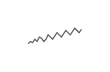
\begin{tikzpicture}[x=0.08em, y=0.08em, line width=0.4pt]
                \draw[FooterGray] (0,3) -- (1,4) -- (2,3.5) -- (3,5) -- (4,4) -- (5,6) -- (6,5.5) -- (7,4) -- (8,5) -- (9,7) -- (10,6) -- (11,5) -- (12,6.5) -- (13,8) -- (14,7) -- (15,6) -- (16,7.5) -- (17,9) -- (18,8) -- (19,7) -- (20,8.5) -- (21,10) -- (22,9) -- (23,8) -- (24,9.5);
            \end{tikzpicture}%
        }%
        \hskip0.5cm%
    }%
    \vskip6pt%
}

%=============================================================================
% PACKAGES
%=============================================================================
\usepackage[utf8]{inputenc}
\DeclareUnicodeCharacter{03B1}{\ensuremath{\alpha}}
\usepackage[T1]{fontenc}
\usepackage{amsmath, amssymb, amsthm}
\usepackage{mathtools}
\usepackage{bm}
\usepackage{tikz}
\usetikzlibrary{arrows.meta, positioning, shapes, calc, decorations.pathreplacing, shadings}
\usepackage{booktabs}
\usepackage{multirow}
\usepackage{array}
\usepackage{graphicx}
\usepackage{animate}
\usepackage{hyperref}
\usepackage{colortbl}
\usepackage{listings}
\lstset{language=Python, basicstyle=\ttfamily\scriptsize, keywordstyle=\color{MainBlue}\bfseries,
  commentstyle=\color{Forest}, stringstyle=\color{Crimson}, breaklines=true,
  frame=none, backgroundcolor=\color{VeryLightGray}, xleftmargin=2mm}
\hypersetup{colorlinks=true, linkcolor=MainBlue, urlcolor=MainBlue}
\graphicspath{{../../logos/}{../../charts/}{../../photos/}}
\usepackage{xcolor}
\hfuzz=2pt  % Suppress tiny overfull warnings (<2pt)
\vfuzz=2pt  % Suppress tiny vertical overfull warnings (<2pt)
% \mathrm in the sans-serif family of the slides (beamer resets \mathrm to the serif family at \begin{document};
% this hook runs after beamer's, so WN, Var, RMSE, ... in formulas match the surrounding text)
% Bold vectors and matrices in the same sans-serif family: \mathbf{A} in sans bold (beamer's own \mathbf came out in
% medium weight), and the bold upright Greek capitals of \boldsymbol / \bm (\bSigma, \bPhi, \boldsymbol{\Theta}) in
% cmss bold: bm.sty fixes its "boldoperators" font when it is loaded (serif cmbx), before beamer switches the
% operators to cmss, so it is reset here.
\AtBeginDocument{%
  \SetMathAlphabet{\mathrm}{normal}{\encodingdefault}{\sfdefault}{\mddefault}{n}%
  \SetMathAlphabet{\mathrm}{bold}{\encodingdefault}{\sfdefault}{bx}{n}%
  \SetMathAlphabet{\mathbf}{normal}{\encodingdefault}{\sfdefault}{bx}{n}%
  \SetMathAlphabet{\mathbf}{bold}{\encodingdefault}{\sfdefault}{bx}{n}%
  \SetSymbolFont{boldoperators}{normal}{OT1}{cmss}{bx}{n}%
  \SetSymbolFont{boldoperators}{bold}{OT1}{cmss}{bx}{n}}

%=============================================================================
% QUANTLET COMMANDS
%   \quantlet{<displayed name>}{<url>}       (generic, compatible with the older TSA decks)
%   \tsaquantlet{Ch_05}{TSA_ch5_garch}       -> https://github.com/danpele/Time-Series-Analysis/tree/main/Quantlets/Ch_05/TSA_ch5_garch
%   \qlurl{<folder>} is defined per chapter by the generator (Quantlets/Ch_NN/<folder>)
%=============================================================================
\newcommand{\tsarepo}{https://github.com/danpele/Time-Series-Analysis}
\newcommand{\tsaqlbase}{https://github.com/danpele/Time-Series-Analysis/tree/main/Quantlets}
\newcommand{\quantlet}[2]{%
    \hfill\href{#2}{%
        \raisebox{-0.15em}{
\includegraphics[height=0.7em]{ql_logo.png}}%
        \textcolor{MainBlue}{\tiny\ #1}%
    }%
}
\newcommand{\tsaquantlet}[2]{\quantlet{\detokenize{#2}}{\tsaqlbase/#1/#2}}

%=============================================================================
% NOTEBOOKS (Google Colab)
%   \colaburl{notebooks/EN/chapter5_seminar_notebook.ipynb} -> the Colab link of a file in the TSA repo
%   \nb: the chapter notebook (each seminar deck redefines it with \renewcommand)
%=============================================================================
\newcommand{\colaburl}[1]{https://colab.research.google.com/github/danpele/Time-Series-Analysis/blob/main/#1}
\newcommand{\nb}{https://colab.research.google.com/github/danpele/Time-Series-Analysis/tree/main/notebooks/EN}
\newcommand{\nbname}{notebooks/EN}

%=============================================================================
% SLIDE HELPERS (used by the generators; the same as in MFM)
%=============================================================================
% local font size for list bodies (the preamble forces \normalsize)
\newcommand{\itemsize}[1]{\setbeamertemplate{itemize/enumerate body begin}{#1}\setbeamertemplate{itemize/enumerate subbody begin}{#1}}
\newcommand{\intitle}[1]{{\hypersetup{urlcolor=white}#1}}   % white links inside coloured title bars
\newcommand{\imgcap}[1]{{\scriptsize #1}\\[0.5mm]}          % caption under a photo
\newcommand{\imgcredit}[2]{{\tiny\color{FooterGray}\href{#1}{#2}}}   % image credit: source URL, author/licence
\newcommand{\aiprompt}[1]{{\ttfamily\color{MainBlue}#1}}     % a prompt to an AI assistant

%=============================================================================
% SEMINARS: student version by default; the instructor wrapper *_solutions.tex sets \solutionstrue
%=============================================================================
\makeatletter\@ifundefined{ifsolutions}{\expandafter\newif\csname ifsolutions\endcsname}{}\makeatother
\newcommand{\solonly}[1]{\ifsolutions #1\fi}
\newcommand{\propsub}{\ifsolutions\else\framesubtitle{\ifdefined\tsalang Rezolvarea se discută la seminar\else Solution discussed in class\fi}\fi}

%=============================================================================
% APPENDIX AND CHAPTER LINKS (latex/appendix_links.py writes the calls; it also re-declares these
% macros before \begin{document}, so the decks compile with or without this preamble block)
%=============================================================================
\providecommand{\tsaapplink}[3]{\hypertarget{#2}{}\hyperlink{#1}{\beamergotobutton{#3}}}
\providecommand{\tsaappback}[2]{\begin{tikzpicture}[remember picture,overlay]\node[anchor=south east] at ([xshift=-3mm,yshift=7mm]current page.south east){\hyperlink{#1}{\beamerreturnbutton{#2}}};\end{tikzpicture}}
\providecommand{\tsachlink}[2]{\href{#1}{#2}}
\providecommand{\tsachlinkt}[2]{\href{#1}{\usebeamercolor[fg]{frametitle}#2}}

%=============================================================================
% QUANTINAR COMMAND: link către un curs Quantinar (subiecte avansate)
%=============================================================================
\newcommand{\quantinar}[2]{%
    \href{#2}{%
        \raisebox{-0.15em}{
\includegraphics[height=0.8em]{qr_logo.png}}%
        \textcolor{MainBlue}{\scriptsize\ #1}%
    }%
}

%=============================================================================
% CUSTOM TITLE PAGE
%=============================================================================
\defbeamertemplate*{title page}{hybrid}[1][]
{
    \vspace{0.2cm}
    % Logos row - top header (with clickable links)
    \begin{center}
        \href{https://www.ase.ro}{
\includegraphics[height=1.0cm]{ase_logo.png}}\hspace{0.3cm}%
        \href{https://theida.net}{
\includegraphics[height=1.0cm]{ida_logo.png}}\hspace{0.3cm}%
        \href{https://blockchain-research-center.com}{
\includegraphics[height=1.0cm]{brc_logo.png}}\hspace{0.3cm}%
        \href{https://www.ai4efin.ase.ro}{
\includegraphics[height=1.0cm]{ai4efin_logo.png}}\hspace{0.3cm}%
        \href{https://ipe.ro/new}{
\includegraphics[height=1.0cm]{acad_logo.png}}\hspace{0.3cm}%
        \href{https://www.digital-finance-msca.com}{
\includegraphics[height=1.0cm]{msca_logo.png}}%
    \end{center}

    \vspace{0.6cm}

    % Main title with Q logos on sides (with clickable links)
    \begin{center}
        \begin{minipage}{0.1\textwidth}
            \centering
            \href{https://quantlet.com}{
\includegraphics[height=1.1cm]{ql_logo.png}}
        \end{minipage}%
        \begin{minipage}{0.78\textwidth}
            \centering
            {\LARGE\bfseries\usebeamercolor[fg]{title}\inserttitle}

            \vspace{0.3cm}

            {\usebeamerfont{subtitle}\usebeamercolor[fg]{title}\insertsubtitle}
        \end{minipage}%
        \begin{minipage}{0.1\textwidth}
            \centering
            \href{https://quantinar.com}{
\includegraphics[height=1.1cm]{qr_logo.png}}
        \end{minipage}
    \end{center}

    \vspace{0.6cm}

    % Authors (left aligned)
    \hspace{0.5cm}{\usebeamerfont{author}\insertauthor}

    \vspace{0.3cm}

    % Institute/Affiliations (left aligned)
    \hspace{0.5cm}\begin{minipage}[t]{0.9\textwidth}
        \raggedright\small\insertinstitute
    \end{minipage}
}

%=============================================================================
% THEOREM ENVIRONMENTS
%=============================================================================
\theoremstyle{definition}
\setbeamertemplate{theorems}[numbered]
\ifdefined\tsalang
\newtheorem{defn}{Definiție}
\newtheorem{thm}{Teoremă}
\newtheorem{prop}{Propoziție}
\newtheorem{rmk}{Observație}
\else
\newtheorem{defn}{Definition}
\newtheorem{thm}{Theorem}
\newtheorem{prop}{Proposition}
\newtheorem{rmk}{Remark}
\fi

%=============================================================================
% CENTRED MINIPAGE (no extra vertical space)
%=============================================================================
\newenvironment{cminipage}[1]{%
    \par\noindent\hfill\begin{minipage}{#1}\ignorespaces
}{%
    \end{minipage}\hfill\null\par
}

%=============================================================================
% CUSTOM COMMANDS
%=============================================================================
\newcommand{\E}{\mathbb{E}}
\newcommand{\Var}{\text{Var}}
\newcommand{\Cov}{\text{Cov}}
\newcommand{\Corr}{\text{Corr}}
\newcommand{\R}{\mathbb{R}}
\newcommand{\N}{\mathbb{N}}
\newcommand{\Z}{\mathbb{Z}}
\newcommand{\B}{\mathbf{B}}
\newcommand{\imark}{\textcolor{MainBlue}{\textbullet}}
\newcommand{\RMSE}{\text{RMSE}}
\newcommand{\MAE}{\text{MAE}}
\newcommand{\MAPE}{\text{MAPE}}

% Boldface vector/matrix commands (VAR, VECM, state space; also used by the older TSA decks)
\newcommand{\bY}{\mathbf{Y}}
\newcommand{\bX}{\mathbf{X}}
\newcommand{\bA}{\mathbf{A}}
\newcommand{\bB}{\mathbf{B}}
\newcommand{\bepsilon}{\boldsymbol{\varepsilon}}
\newcommand{\bSigma}{\boldsymbol{\Sigma}}
\newcommand{\bPhi}{\boldsymbol{\Phi}}
\newcommand{\bGamma}{\boldsymbol{\Gamma}}
\newcommand{\bPi}{\boldsymbol{\Pi}}
\newcommand{\bc}{\mathbf{c}}
\newcommand{\balpha}{\boldsymbol{\alpha}}
\newcommand{\bbeta}{\boldsymbol{\beta}}
\newcommand{\bvarepsilon}{\boldsymbol{\varepsilon}}

% Legacy seminar marks (older TSA seminar decks)
\newcommand{\correct}{\textcolor{Forest}{\checkmark}}
\newcommand{\incorrect}{\textcolor{Crimson}{\texttimes}}
 se definește
%   \newcommand{\coursename}{Time Series Analysis}      (EN)
%   \newcommand{\coursename}{Serii de timp}       (RO)  și  \def\tsalang{ro}
% Fișierele .tex se află în EN/Courses, EN/Seminars, RO/Cursuri, RO/Seminarii (două niveluri sub rădăcină).
% Deck-urile sînt generate de latex/build_chapterN.py / build_seminarN.py (vezi latex/tsa_build.py).

\documentclass[9pt, aspectratio=169, t]{beamer}
\providecommand{\coursename}{Time Series Analysis}

% Ensure content fits on slides
\setbeamersize{text margin left=8mm, text margin right=8mm}
% Smaller institute font (title page)
\setbeamerfont{institute}{size=\footnotesize}

%=============================================================================
% THEME AND STYLE CONFIGURATION
%=============================================================================
\usetheme{default}
% Using default theme for clean header/footer control

% Color Palette (matching Redispatch PDF)
\definecolor{MainBlue}{RGB}{26, 58, 110}
\definecolor{AccentBlue}{RGB}{26, 58, 110}
\definecolor{IDAred}{RGB}{205, 0, 0}
\definecolor{DarkGray}{RGB}{51, 51, 51}
\definecolor{MediumGray}{RGB}{128, 128, 128}
\definecolor{LightGray}{RGB}{248, 248, 248}
\definecolor{VeryLightGray}{RGB}{235, 235, 235}
\definecolor{KeynoteGray}{RGB}{218, 218, 218}
\definecolor{SectionGray}{RGB}{120, 120, 120}
\definecolor{FooterGray}{RGB}{100, 100, 100}
\definecolor{Crimson}{RGB}{220, 53, 69}
\definecolor{Forest}{RGB}{46, 125, 50}
\definecolor{Amber}{RGB}{181, 133, 63}
\definecolor{Orange}{RGB}{230, 126, 34}
\definecolor{Purple}{RGB}{142, 68, 173}

% Gradient background (exact Keynote 315° gradient: white to RGB 218,218,218)
\setbeamertemplate{background}{%
    \begin{tikzpicture}[remember picture, overlay]
        \shade[shading=axis, shading angle=315,
        top color=white, bottom color=KeynoteGray]
        (current page.south west) rectangle (current page.north east);
    \end{tikzpicture}%
}
% Fallback solid color for compatibility
\setbeamercolor{background canvas}{bg=}

\setbeamercolor{palette primary}{bg=MainBlue, fg=white}
\setbeamercolor{palette secondary}{bg=MainBlue!85, fg=white}
\setbeamercolor{palette tertiary}{bg=MainBlue!70, fg=white}
\setbeamercolor{structure}{fg=MainBlue}
\setbeamercolor{title}{fg=IDAred}
\setbeamercolor{frametitle}{fg=IDAred, bg=}
\setbeamercolor{block title}{bg=MainBlue, fg=white}
\setbeamercolor{block body}{bg=VeryLightGray, fg=DarkGray}
\setbeamercolor{block title alerted}{bg=Crimson, fg=white}
\setbeamercolor{block body alerted}{bg=Crimson!8, fg=DarkGray}
\setbeamercolor{block title example}{bg=Forest, fg=white}
\setbeamercolor{block body example}{bg=Forest!8, fg=DarkGray}
\setbeamercolor{item}{fg=MainBlue}

% Footer colors (override Madrid theme blue)
\setbeamercolor{author in head/foot}{fg=FooterGray, bg=}
\setbeamercolor{title in head/foot}{fg=FooterGray, bg=}
\setbeamercolor{date in head/foot}{fg=FooterGray, bg=}
\setbeamercolor{section in head/foot}{fg=FooterGray, bg=}
\setbeamercolor{subsection in head/foot}{fg=FooterGray, bg=}

% Bullet styles (apply everywhere including blocks)
\setbeamertemplate{itemize item}{\color{MainBlue}$\boxdot$}
\setbeamertemplate{itemize subitem}{\color{MainBlue}$\blacktriangleright$}
\setbeamertemplate{itemize subsubitem}{\color{MainBlue}\tiny$\bullet$}
\setbeamertemplate{itemize/enumerate body begin}{\normalsize}
\setbeamertemplate{itemize/enumerate subbody begin}{\normalsize}

% Item spacing - compact style
\setlength{\leftmargini}{10pt}       % Level 1: minimal indent
\setlength{\leftmarginii}{10pt}      % Level 2: minimal additional indent
% Compact list spacing (zero extra space before/after lists in blocks)
\makeatletter
\def\@listi{\leftmargin\leftmargini \topsep 0pt \parsep 0pt \itemsep 0pt}
\def\@listii{\leftmargin\leftmarginii \topsep 0pt \parsep 0pt \itemsep 0pt}
\makeatother

\setbeamertemplate{navigation symbols}{}

%=============================================================================
% CUSTOM HEADLINE
%=============================================================================
\setbeamertemplate{headline}{%
    \vskip10pt%
    \hbox to \paperwidth{%
        \hskip0.5cm%
        {\small\color{FooterGray}\renewcommand{\hyperlink}[2]{##2}\insertsectionhead}%
        \hfill%
        \textcolor{FooterGray}{\small\insertframenumber}%
        \hskip0.5cm%
    }%
    \vskip4pt%
    {\color{FooterGray}\hrule height 0.4pt}%
}

%=============================================================================
% CUSTOM FOOTER
%=============================================================================
\usepackage{fontawesome5}

\setbeamertemplate{footline}{%
    {\color{FooterGray}\hrule height 0.4pt}%
    \vskip4pt%
    \hbox to \paperwidth{%
        \hskip0.5cm%
        \textcolor{FooterGray}{\small\coursename}%
        \hfill%
        \raisebox{-0.1em}{%
            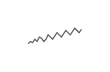
\begin{tikzpicture}[x=0.08em, y=0.08em, line width=0.4pt]
                \draw[FooterGray] (0,3) -- (1,4) -- (2,3.5) -- (3,5) -- (4,4) -- (5,6) -- (6,5.5) -- (7,4) -- (8,5) -- (9,7) -- (10,6) -- (11,5) -- (12,6.5) -- (13,8) -- (14,7) -- (15,6) -- (16,7.5) -- (17,9) -- (18,8) -- (19,7) -- (20,8.5) -- (21,10) -- (22,9) -- (23,8) -- (24,9.5);
            \end{tikzpicture}%
        }%
        \hskip0.5cm%
    }%
    \vskip6pt%
}

%=============================================================================
% PACKAGES
%=============================================================================
\usepackage[utf8]{inputenc}
\DeclareUnicodeCharacter{03B1}{\ensuremath{\alpha}}
\usepackage[T1]{fontenc}
\usepackage{amsmath, amssymb, amsthm}
\usepackage{mathtools}
\usepackage{bm}
\usepackage{tikz}
\usetikzlibrary{arrows.meta, positioning, shapes, calc, decorations.pathreplacing, shadings}
\usepackage{booktabs}
\usepackage{multirow}
\usepackage{array}
\usepackage{graphicx}
\usepackage{animate}
\usepackage{hyperref}
\usepackage{colortbl}
\usepackage{listings}
\lstset{language=Python, basicstyle=\ttfamily\scriptsize, keywordstyle=\color{MainBlue}\bfseries,
  commentstyle=\color{Forest}, stringstyle=\color{Crimson}, breaklines=true,
  frame=none, backgroundcolor=\color{VeryLightGray}, xleftmargin=2mm}
\hypersetup{colorlinks=true, linkcolor=MainBlue, urlcolor=MainBlue}
\graphicspath{{../../logos/}{../../charts/}{../../photos/}}
\usepackage{xcolor}
\hfuzz=2pt  % Suppress tiny overfull warnings (<2pt)
\vfuzz=2pt  % Suppress tiny vertical overfull warnings (<2pt)
% \mathrm in the sans-serif family of the slides (beamer resets \mathrm to the serif family at \begin{document};
% this hook runs after beamer's, so WN, Var, RMSE, ... in formulas match the surrounding text)
% Bold vectors and matrices in the same sans-serif family: \mathbf{A} in sans bold (beamer's own \mathbf came out in
% medium weight), and the bold upright Greek capitals of \boldsymbol / \bm (\bSigma, \bPhi, \boldsymbol{\Theta}) in
% cmss bold: bm.sty fixes its "boldoperators" font when it is loaded (serif cmbx), before beamer switches the
% operators to cmss, so it is reset here.
\AtBeginDocument{%
  \SetMathAlphabet{\mathrm}{normal}{\encodingdefault}{\sfdefault}{\mddefault}{n}%
  \SetMathAlphabet{\mathrm}{bold}{\encodingdefault}{\sfdefault}{bx}{n}%
  \SetMathAlphabet{\mathbf}{normal}{\encodingdefault}{\sfdefault}{bx}{n}%
  \SetMathAlphabet{\mathbf}{bold}{\encodingdefault}{\sfdefault}{bx}{n}%
  \SetSymbolFont{boldoperators}{normal}{OT1}{cmss}{bx}{n}%
  \SetSymbolFont{boldoperators}{bold}{OT1}{cmss}{bx}{n}}

%=============================================================================
% QUANTLET COMMANDS
%   \quantlet{<displayed name>}{<url>}       (generic, compatible with the older TSA decks)
%   \tsaquantlet{Ch_05}{TSA_ch5_garch}       -> https://github.com/danpele/Time-Series-Analysis/tree/main/Quantlets/Ch_05/TSA_ch5_garch
%   \qlurl{<folder>} is defined per chapter by the generator (Quantlets/Ch_NN/<folder>)
%=============================================================================
\newcommand{\tsarepo}{https://github.com/danpele/Time-Series-Analysis}
\newcommand{\tsaqlbase}{https://github.com/danpele/Time-Series-Analysis/tree/main/Quantlets}
\newcommand{\quantlet}[2]{%
    \hfill\href{#2}{%
        \raisebox{-0.15em}{
\includegraphics[height=0.7em]{ql_logo.png}}%
        \textcolor{MainBlue}{\tiny\ #1}%
    }%
}
\newcommand{\tsaquantlet}[2]{\quantlet{\detokenize{#2}}{\tsaqlbase/#1/#2}}

%=============================================================================
% NOTEBOOKS (Google Colab)
%   \colaburl{notebooks/EN/chapter5_seminar_notebook.ipynb} -> the Colab link of a file in the TSA repo
%   \nb: the chapter notebook (each seminar deck redefines it with \renewcommand)
%=============================================================================
\newcommand{\colaburl}[1]{https://colab.research.google.com/github/danpele/Time-Series-Analysis/blob/main/#1}
\newcommand{\nb}{https://colab.research.google.com/github/danpele/Time-Series-Analysis/tree/main/notebooks/EN}
\newcommand{\nbname}{notebooks/EN}

%=============================================================================
% SLIDE HELPERS (used by the generators; the same as in MFM)
%=============================================================================
% local font size for list bodies (the preamble forces \normalsize)
\newcommand{\itemsize}[1]{\setbeamertemplate{itemize/enumerate body begin}{#1}\setbeamertemplate{itemize/enumerate subbody begin}{#1}}
\newcommand{\intitle}[1]{{\hypersetup{urlcolor=white}#1}}   % white links inside coloured title bars
\newcommand{\imgcap}[1]{{\scriptsize #1}\\[0.5mm]}          % caption under a photo
\newcommand{\imgcredit}[2]{{\tiny\color{FooterGray}\href{#1}{#2}}}   % image credit: source URL, author/licence
\newcommand{\aiprompt}[1]{{\ttfamily\color{MainBlue}#1}}     % a prompt to an AI assistant

%=============================================================================
% SEMINARS: student version by default; the instructor wrapper *_solutions.tex sets \solutionstrue
%=============================================================================
\makeatletter\@ifundefined{ifsolutions}{\expandafter\newif\csname ifsolutions\endcsname}{}\makeatother
\newcommand{\solonly}[1]{\ifsolutions #1\fi}
\newcommand{\propsub}{\ifsolutions\else\framesubtitle{\ifdefined\tsalang Rezolvarea se discută la seminar\else Solution discussed in class\fi}\fi}

%=============================================================================
% APPENDIX AND CHAPTER LINKS (latex/appendix_links.py writes the calls; it also re-declares these
% macros before \begin{document}, so the decks compile with or without this preamble block)
%=============================================================================
\providecommand{\tsaapplink}[3]{\hypertarget{#2}{}\hyperlink{#1}{\beamergotobutton{#3}}}
\providecommand{\tsaappback}[2]{\begin{tikzpicture}[remember picture,overlay]\node[anchor=south east] at ([xshift=-3mm,yshift=7mm]current page.south east){\hyperlink{#1}{\beamerreturnbutton{#2}}};\end{tikzpicture}}
\providecommand{\tsachlink}[2]{\href{#1}{#2}}
\providecommand{\tsachlinkt}[2]{\href{#1}{\usebeamercolor[fg]{frametitle}#2}}

%=============================================================================
% QUANTINAR COMMAND: link către un curs Quantinar (subiecte avansate)
%=============================================================================
\newcommand{\quantinar}[2]{%
    \href{#2}{%
        \raisebox{-0.15em}{
\includegraphics[height=0.8em]{qr_logo.png}}%
        \textcolor{MainBlue}{\scriptsize\ #1}%
    }%
}

%=============================================================================
% CUSTOM TITLE PAGE
%=============================================================================
\defbeamertemplate*{title page}{hybrid}[1][]
{
    \vspace{0.2cm}
    % Logos row - top header (with clickable links)
    \begin{center}
        \href{https://www.ase.ro}{
\includegraphics[height=1.0cm]{ase_logo.png}}\hspace{0.3cm}%
        \href{https://theida.net}{
\includegraphics[height=1.0cm]{ida_logo.png}}\hspace{0.3cm}%
        \href{https://blockchain-research-center.com}{
\includegraphics[height=1.0cm]{brc_logo.png}}\hspace{0.3cm}%
        \href{https://www.ai4efin.ase.ro}{
\includegraphics[height=1.0cm]{ai4efin_logo.png}}\hspace{0.3cm}%
        \href{https://ipe.ro/new}{
\includegraphics[height=1.0cm]{acad_logo.png}}\hspace{0.3cm}%
        \href{https://www.digital-finance-msca.com}{
\includegraphics[height=1.0cm]{msca_logo.png}}%
    \end{center}

    \vspace{0.6cm}

    % Main title with Q logos on sides (with clickable links)
    \begin{center}
        \begin{minipage}{0.1\textwidth}
            \centering
            \href{https://quantlet.com}{
\includegraphics[height=1.1cm]{ql_logo.png}}
        \end{minipage}%
        \begin{minipage}{0.78\textwidth}
            \centering
            {\LARGE\bfseries\usebeamercolor[fg]{title}\inserttitle}

            \vspace{0.3cm}

            {\usebeamerfont{subtitle}\usebeamercolor[fg]{title}\insertsubtitle}
        \end{minipage}%
        \begin{minipage}{0.1\textwidth}
            \centering
            \href{https://quantinar.com}{
\includegraphics[height=1.1cm]{qr_logo.png}}
        \end{minipage}
    \end{center}

    \vspace{0.6cm}

    % Authors (left aligned)
    \hspace{0.5cm}{\usebeamerfont{author}\insertauthor}

    \vspace{0.3cm}

    % Institute/Affiliations (left aligned)
    \hspace{0.5cm}\begin{minipage}[t]{0.9\textwidth}
        \raggedright\small\insertinstitute
    \end{minipage}
}

%=============================================================================
% THEOREM ENVIRONMENTS
%=============================================================================
\theoremstyle{definition}
\setbeamertemplate{theorems}[numbered]
\ifdefined\tsalang
\newtheorem{defn}{Definiție}
\newtheorem{thm}{Teoremă}
\newtheorem{prop}{Propoziție}
\newtheorem{rmk}{Observație}
\else
\newtheorem{defn}{Definition}
\newtheorem{thm}{Theorem}
\newtheorem{prop}{Proposition}
\newtheorem{rmk}{Remark}
\fi

%=============================================================================
% CENTRED MINIPAGE (no extra vertical space)
%=============================================================================
\newenvironment{cminipage}[1]{%
    \par\noindent\hfill\begin{minipage}{#1}\ignorespaces
}{%
    \end{minipage}\hfill\null\par
}

%=============================================================================
% CUSTOM COMMANDS
%=============================================================================
\newcommand{\E}{\mathbb{E}}
\newcommand{\Var}{\text{Var}}
\newcommand{\Cov}{\text{Cov}}
\newcommand{\Corr}{\text{Corr}}
\newcommand{\R}{\mathbb{R}}
\newcommand{\N}{\mathbb{N}}
\newcommand{\Z}{\mathbb{Z}}
\newcommand{\B}{\mathbf{B}}
\newcommand{\imark}{\textcolor{MainBlue}{\textbullet}}
\newcommand{\RMSE}{\text{RMSE}}
\newcommand{\MAE}{\text{MAE}}
\newcommand{\MAPE}{\text{MAPE}}

% Boldface vector/matrix commands (VAR, VECM, state space; also used by the older TSA decks)
\newcommand{\bY}{\mathbf{Y}}
\newcommand{\bX}{\mathbf{X}}
\newcommand{\bA}{\mathbf{A}}
\newcommand{\bB}{\mathbf{B}}
\newcommand{\bepsilon}{\boldsymbol{\varepsilon}}
\newcommand{\bSigma}{\boldsymbol{\Sigma}}
\newcommand{\bPhi}{\boldsymbol{\Phi}}
\newcommand{\bGamma}{\boldsymbol{\Gamma}}
\newcommand{\bPi}{\boldsymbol{\Pi}}
\newcommand{\bc}{\mathbf{c}}
\newcommand{\balpha}{\boldsymbol{\alpha}}
\newcommand{\bbeta}{\boldsymbol{\beta}}
\newcommand{\bvarepsilon}{\boldsymbol{\varepsilon}}

% Legacy seminar marks (older TSA seminar decks)
\newcommand{\correct}{\textcolor{Forest}{\checkmark}}
\newcommand{\incorrect}{\textcolor{Crimson}{\texttimes}}
 se definește
%   \newcommand{\coursename}{Time Series Analysis}      (EN)
%   \newcommand{\coursename}{Serii de timp}       (RO)  și  \def\tsalang{ro}
% Fișierele .tex se află în EN/Courses, EN/Seminars, RO/Cursuri, RO/Seminarii (două niveluri sub rădăcină).
% Deck-urile sînt generate de latex/build_chapterN.py / build_seminarN.py (vezi latex/tsa_build.py).

\documentclass[9pt, aspectratio=169, t]{beamer}
\providecommand{\coursename}{Time Series Analysis}

% Ensure content fits on slides
\setbeamersize{text margin left=8mm, text margin right=8mm}
% Smaller institute font (title page)
\setbeamerfont{institute}{size=\footnotesize}

%=============================================================================
% THEME AND STYLE CONFIGURATION
%=============================================================================
\usetheme{default}
% Using default theme for clean header/footer control

% Color Palette (matching Redispatch PDF)
\definecolor{MainBlue}{RGB}{26, 58, 110}
\definecolor{AccentBlue}{RGB}{26, 58, 110}
\definecolor{IDAred}{RGB}{205, 0, 0}
\definecolor{DarkGray}{RGB}{51, 51, 51}
\definecolor{MediumGray}{RGB}{128, 128, 128}
\definecolor{LightGray}{RGB}{248, 248, 248}
\definecolor{VeryLightGray}{RGB}{235, 235, 235}
\definecolor{KeynoteGray}{RGB}{218, 218, 218}
\definecolor{SectionGray}{RGB}{120, 120, 120}
\definecolor{FooterGray}{RGB}{100, 100, 100}
\definecolor{Crimson}{RGB}{220, 53, 69}
\definecolor{Forest}{RGB}{46, 125, 50}
\definecolor{Amber}{RGB}{181, 133, 63}
\definecolor{Orange}{RGB}{230, 126, 34}
\definecolor{Purple}{RGB}{142, 68, 173}

% Gradient background (exact Keynote 315° gradient: white to RGB 218,218,218)
\setbeamertemplate{background}{%
    \begin{tikzpicture}[remember picture, overlay]
        \shade[shading=axis, shading angle=315,
        top color=white, bottom color=KeynoteGray]
        (current page.south west) rectangle (current page.north east);
    \end{tikzpicture}%
}
% Fallback solid color for compatibility
\setbeamercolor{background canvas}{bg=}

\setbeamercolor{palette primary}{bg=MainBlue, fg=white}
\setbeamercolor{palette secondary}{bg=MainBlue!85, fg=white}
\setbeamercolor{palette tertiary}{bg=MainBlue!70, fg=white}
\setbeamercolor{structure}{fg=MainBlue}
\setbeamercolor{title}{fg=IDAred}
\setbeamercolor{frametitle}{fg=IDAred, bg=}
\setbeamercolor{block title}{bg=MainBlue, fg=white}
\setbeamercolor{block body}{bg=VeryLightGray, fg=DarkGray}
\setbeamercolor{block title alerted}{bg=Crimson, fg=white}
\setbeamercolor{block body alerted}{bg=Crimson!8, fg=DarkGray}
\setbeamercolor{block title example}{bg=Forest, fg=white}
\setbeamercolor{block body example}{bg=Forest!8, fg=DarkGray}
\setbeamercolor{item}{fg=MainBlue}

% Footer colors (override Madrid theme blue)
\setbeamercolor{author in head/foot}{fg=FooterGray, bg=}
\setbeamercolor{title in head/foot}{fg=FooterGray, bg=}
\setbeamercolor{date in head/foot}{fg=FooterGray, bg=}
\setbeamercolor{section in head/foot}{fg=FooterGray, bg=}
\setbeamercolor{subsection in head/foot}{fg=FooterGray, bg=}

% Bullet styles (apply everywhere including blocks)
\setbeamertemplate{itemize item}{\color{MainBlue}$\boxdot$}
\setbeamertemplate{itemize subitem}{\color{MainBlue}$\blacktriangleright$}
\setbeamertemplate{itemize subsubitem}{\color{MainBlue}\tiny$\bullet$}
\setbeamertemplate{itemize/enumerate body begin}{\normalsize}
\setbeamertemplate{itemize/enumerate subbody begin}{\normalsize}

% Item spacing - compact style
\setlength{\leftmargini}{10pt}       % Level 1: minimal indent
\setlength{\leftmarginii}{10pt}      % Level 2: minimal additional indent
% Compact list spacing (zero extra space before/after lists in blocks)
\makeatletter
\def\@listi{\leftmargin\leftmargini \topsep 0pt \parsep 0pt \itemsep 0pt}
\def\@listii{\leftmargin\leftmarginii \topsep 0pt \parsep 0pt \itemsep 0pt}
\makeatother

\setbeamertemplate{navigation symbols}{}

%=============================================================================
% CUSTOM HEADLINE
%=============================================================================
\setbeamertemplate{headline}{%
    \vskip10pt%
    \hbox to \paperwidth{%
        \hskip0.5cm%
        {\small\color{FooterGray}\renewcommand{\hyperlink}[2]{##2}\insertsectionhead}%
        \hfill%
        \textcolor{FooterGray}{\small\insertframenumber}%
        \hskip0.5cm%
    }%
    \vskip4pt%
    {\color{FooterGray}\hrule height 0.4pt}%
}

%=============================================================================
% CUSTOM FOOTER
%=============================================================================
\usepackage{fontawesome5}

\setbeamertemplate{footline}{%
    {\color{FooterGray}\hrule height 0.4pt}%
    \vskip4pt%
    \hbox to \paperwidth{%
        \hskip0.5cm%
        \textcolor{FooterGray}{\small\coursename}%
        \hfill%
        \raisebox{-0.1em}{%
            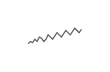
\begin{tikzpicture}[x=0.08em, y=0.08em, line width=0.4pt]
                \draw[FooterGray] (0,3) -- (1,4) -- (2,3.5) -- (3,5) -- (4,4) -- (5,6) -- (6,5.5) -- (7,4) -- (8,5) -- (9,7) -- (10,6) -- (11,5) -- (12,6.5) -- (13,8) -- (14,7) -- (15,6) -- (16,7.5) -- (17,9) -- (18,8) -- (19,7) -- (20,8.5) -- (21,10) -- (22,9) -- (23,8) -- (24,9.5);
            \end{tikzpicture}%
        }%
        \hskip0.5cm%
    }%
    \vskip6pt%
}

%=============================================================================
% PACKAGES
%=============================================================================
\usepackage[utf8]{inputenc}
\DeclareUnicodeCharacter{03B1}{\ensuremath{\alpha}}
\usepackage[T1]{fontenc}
\usepackage{amsmath, amssymb, amsthm}
\usepackage{mathtools}
\usepackage{bm}
\usepackage{tikz}
\usetikzlibrary{arrows.meta, positioning, shapes, calc, decorations.pathreplacing, shadings}
\usepackage{booktabs}
\usepackage{multirow}
\usepackage{array}
\usepackage{graphicx}
\usepackage{animate}
\usepackage{hyperref}
\usepackage{colortbl}
\usepackage{listings}
\lstset{language=Python, basicstyle=\ttfamily\scriptsize, keywordstyle=\color{MainBlue}\bfseries,
  commentstyle=\color{Forest}, stringstyle=\color{Crimson}, breaklines=true,
  frame=none, backgroundcolor=\color{VeryLightGray}, xleftmargin=2mm}
\hypersetup{colorlinks=true, linkcolor=MainBlue, urlcolor=MainBlue}
\graphicspath{{../../logos/}{../../charts/}{../../photos/}}
\usepackage{xcolor}
\hfuzz=2pt  % Suppress tiny overfull warnings (<2pt)
\vfuzz=2pt  % Suppress tiny vertical overfull warnings (<2pt)
% \mathrm in the sans-serif family of the slides (beamer resets \mathrm to the serif family at \begin{document};
% this hook runs after beamer's, so WN, Var, RMSE, ... in formulas match the surrounding text)
% Bold vectors and matrices in the same sans-serif family: \mathbf{A} in sans bold (beamer's own \mathbf came out in
% medium weight), and the bold upright Greek capitals of \boldsymbol / \bm (\bSigma, \bPhi, \boldsymbol{\Theta}) in
% cmss bold: bm.sty fixes its "boldoperators" font when it is loaded (serif cmbx), before beamer switches the
% operators to cmss, so it is reset here.
\AtBeginDocument{%
  \SetMathAlphabet{\mathrm}{normal}{\encodingdefault}{\sfdefault}{\mddefault}{n}%
  \SetMathAlphabet{\mathrm}{bold}{\encodingdefault}{\sfdefault}{bx}{n}%
  \SetMathAlphabet{\mathbf}{normal}{\encodingdefault}{\sfdefault}{bx}{n}%
  \SetMathAlphabet{\mathbf}{bold}{\encodingdefault}{\sfdefault}{bx}{n}%
  \SetSymbolFont{boldoperators}{normal}{OT1}{cmss}{bx}{n}%
  \SetSymbolFont{boldoperators}{bold}{OT1}{cmss}{bx}{n}}

%=============================================================================
% QUANTLET COMMANDS
%   \quantlet{<displayed name>}{<url>}       (generic, compatible with the older TSA decks)
%   \tsaquantlet{Ch_05}{TSA_ch5_garch}       -> https://github.com/danpele/Time-Series-Analysis/tree/main/Quantlets/Ch_05/TSA_ch5_garch
%   \qlurl{<folder>} is defined per chapter by the generator (Quantlets/Ch_NN/<folder>)
%=============================================================================
\newcommand{\tsarepo}{https://github.com/danpele/Time-Series-Analysis}
\newcommand{\tsaqlbase}{https://github.com/danpele/Time-Series-Analysis/tree/main/Quantlets}
\newcommand{\quantlet}[2]{%
    \hfill\href{#2}{%
        \raisebox{-0.15em}{
\includegraphics[height=0.7em]{ql_logo.png}}%
        \textcolor{MainBlue}{\tiny\ #1}%
    }%
}
\newcommand{\tsaquantlet}[2]{\quantlet{\detokenize{#2}}{\tsaqlbase/#1/#2}}

%=============================================================================
% NOTEBOOKS (Google Colab)
%   \colaburl{notebooks/EN/chapter5_seminar_notebook.ipynb} -> the Colab link of a file in the TSA repo
%   \nb: the chapter notebook (each seminar deck redefines it with \renewcommand)
%=============================================================================
\newcommand{\colaburl}[1]{https://colab.research.google.com/github/danpele/Time-Series-Analysis/blob/main/#1}
\newcommand{\nb}{https://colab.research.google.com/github/danpele/Time-Series-Analysis/tree/main/notebooks/EN}
\newcommand{\nbname}{notebooks/EN}

%=============================================================================
% SLIDE HELPERS (used by the generators; the same as in MFM)
%=============================================================================
% local font size for list bodies (the preamble forces \normalsize)
\newcommand{\itemsize}[1]{\setbeamertemplate{itemize/enumerate body begin}{#1}\setbeamertemplate{itemize/enumerate subbody begin}{#1}}
\newcommand{\intitle}[1]{{\hypersetup{urlcolor=white}#1}}   % white links inside coloured title bars
\newcommand{\imgcap}[1]{{\scriptsize #1}\\[0.5mm]}          % caption under a photo
\newcommand{\imgcredit}[2]{{\tiny\color{FooterGray}\href{#1}{#2}}}   % image credit: source URL, author/licence
\newcommand{\aiprompt}[1]{{\ttfamily\color{MainBlue}#1}}     % a prompt to an AI assistant

%=============================================================================
% SEMINARS: student version by default; the instructor wrapper *_solutions.tex sets \solutionstrue
%=============================================================================
\makeatletter\@ifundefined{ifsolutions}{\expandafter\newif\csname ifsolutions\endcsname}{}\makeatother
\newcommand{\solonly}[1]{\ifsolutions #1\fi}
\newcommand{\propsub}{\ifsolutions\else\framesubtitle{\ifdefined\tsalang Rezolvarea se discută la seminar\else Solution discussed in class\fi}\fi}

%=============================================================================
% APPENDIX AND CHAPTER LINKS (latex/appendix_links.py writes the calls; it also re-declares these
% macros before \begin{document}, so the decks compile with or without this preamble block)
%=============================================================================
\providecommand{\tsaapplink}[3]{\hypertarget{#2}{}\hyperlink{#1}{\beamergotobutton{#3}}}
\providecommand{\tsaappback}[2]{\begin{tikzpicture}[remember picture,overlay]\node[anchor=south east] at ([xshift=-3mm,yshift=7mm]current page.south east){\hyperlink{#1}{\beamerreturnbutton{#2}}};\end{tikzpicture}}
\providecommand{\tsachlink}[2]{\href{#1}{#2}}
\providecommand{\tsachlinkt}[2]{\href{#1}{\usebeamercolor[fg]{frametitle}#2}}

%=============================================================================
% QUANTINAR COMMAND: link către un curs Quantinar (subiecte avansate)
%=============================================================================
\newcommand{\quantinar}[2]{%
    \href{#2}{%
        \raisebox{-0.15em}{
\includegraphics[height=0.8em]{qr_logo.png}}%
        \textcolor{MainBlue}{\scriptsize\ #1}%
    }%
}

%=============================================================================
% CUSTOM TITLE PAGE
%=============================================================================
\defbeamertemplate*{title page}{hybrid}[1][]
{
    \vspace{0.2cm}
    % Logos row - top header (with clickable links)
    \begin{center}
        \href{https://www.ase.ro}{
\includegraphics[height=1.0cm]{ase_logo.png}}\hspace{0.3cm}%
        \href{https://theida.net}{
\includegraphics[height=1.0cm]{ida_logo.png}}\hspace{0.3cm}%
        \href{https://blockchain-research-center.com}{
\includegraphics[height=1.0cm]{brc_logo.png}}\hspace{0.3cm}%
        \href{https://www.ai4efin.ase.ro}{
\includegraphics[height=1.0cm]{ai4efin_logo.png}}\hspace{0.3cm}%
        \href{https://ipe.ro/new}{
\includegraphics[height=1.0cm]{acad_logo.png}}\hspace{0.3cm}%
        \href{https://www.digital-finance-msca.com}{
\includegraphics[height=1.0cm]{msca_logo.png}}%
    \end{center}

    \vspace{0.6cm}

    % Main title with Q logos on sides (with clickable links)
    \begin{center}
        \begin{minipage}{0.1\textwidth}
            \centering
            \href{https://quantlet.com}{
\includegraphics[height=1.1cm]{ql_logo.png}}
        \end{minipage}%
        \begin{minipage}{0.78\textwidth}
            \centering
            {\LARGE\bfseries\usebeamercolor[fg]{title}\inserttitle}

            \vspace{0.3cm}

            {\usebeamerfont{subtitle}\usebeamercolor[fg]{title}\insertsubtitle}
        \end{minipage}%
        \begin{minipage}{0.1\textwidth}
            \centering
            \href{https://quantinar.com}{
\includegraphics[height=1.1cm]{qr_logo.png}}
        \end{minipage}
    \end{center}

    \vspace{0.6cm}

    % Authors (left aligned)
    \hspace{0.5cm}{\usebeamerfont{author}\insertauthor}

    \vspace{0.3cm}

    % Institute/Affiliations (left aligned)
    \hspace{0.5cm}\begin{minipage}[t]{0.9\textwidth}
        \raggedright\small\insertinstitute
    \end{minipage}
}

%=============================================================================
% THEOREM ENVIRONMENTS
%=============================================================================
\theoremstyle{definition}
\setbeamertemplate{theorems}[numbered]
\ifdefined\tsalang
\newtheorem{defn}{Definiție}
\newtheorem{thm}{Teoremă}
\newtheorem{prop}{Propoziție}
\newtheorem{rmk}{Observație}
\else
\newtheorem{defn}{Definition}
\newtheorem{thm}{Theorem}
\newtheorem{prop}{Proposition}
\newtheorem{rmk}{Remark}
\fi

%=============================================================================
% CENTRED MINIPAGE (no extra vertical space)
%=============================================================================
\newenvironment{cminipage}[1]{%
    \par\noindent\hfill\begin{minipage}{#1}\ignorespaces
}{%
    \end{minipage}\hfill\null\par
}

%=============================================================================
% CUSTOM COMMANDS
%=============================================================================
\newcommand{\E}{\mathbb{E}}
\newcommand{\Var}{\text{Var}}
\newcommand{\Cov}{\text{Cov}}
\newcommand{\Corr}{\text{Corr}}
\newcommand{\R}{\mathbb{R}}
\newcommand{\N}{\mathbb{N}}
\newcommand{\Z}{\mathbb{Z}}
\newcommand{\B}{\mathbf{B}}
\newcommand{\imark}{\textcolor{MainBlue}{\textbullet}}
\newcommand{\RMSE}{\text{RMSE}}
\newcommand{\MAE}{\text{MAE}}
\newcommand{\MAPE}{\text{MAPE}}

% Boldface vector/matrix commands (VAR, VECM, state space; also used by the older TSA decks)
\newcommand{\bY}{\mathbf{Y}}
\newcommand{\bX}{\mathbf{X}}
\newcommand{\bA}{\mathbf{A}}
\newcommand{\bB}{\mathbf{B}}
\newcommand{\bepsilon}{\boldsymbol{\varepsilon}}
\newcommand{\bSigma}{\boldsymbol{\Sigma}}
\newcommand{\bPhi}{\boldsymbol{\Phi}}
\newcommand{\bGamma}{\boldsymbol{\Gamma}}
\newcommand{\bPi}{\boldsymbol{\Pi}}
\newcommand{\bc}{\mathbf{c}}
\newcommand{\balpha}{\boldsymbol{\alpha}}
\newcommand{\bbeta}{\boldsymbol{\beta}}
\newcommand{\bvarepsilon}{\boldsymbol{\varepsilon}}

% Legacy seminar marks (older TSA seminar decks)
\newcommand{\correct}{\textcolor{Forest}{\checkmark}}
\newcommand{\incorrect}{\textcolor{Crimson}{\texttimes}}


\newcommand{\qlurl}[1]{https://github.com/danpele/Time-Series-Analysis/tree/main/Quantlets/Ch_09/#1}

% Clickable citations (DOIs verified via Crossref)
\newcommand{\refHP}{\href{https://doi.org/10.1007/978-3-031-13584-2}{Huang și Petukhina (2022)}}
\newcommand{\refFPP}{\href{https://otexts.com/fpp3/nnetar.html}{Hyndman și Athanasopoulos (2021)}}
\newcommand{\refESL}{\href{https://doi.org/10.1007/978-0-387-84858-7}{Hastie, Tibshirani și Friedman (2009)}}
\newcommand{\refHK}{\href{https://doi.org/10.1016/j.ijforecast.2006.03.001}{Hyndman și Koehler (2006)}}
\newcommand{\refDM}{\href{https://doi.org/10.1080/07350015.1995.10524599}{Diebold și Mariano (1995)}}
\newcommand{\refHLN}{\href{https://doi.org/10.1016/S0169-2070(96)00719-4}{Harvey, Leybourne și Newbold (1997)}}
\newcommand{\refBHK}{\href{https://doi.org/10.1016/j.csda.2017.11.003}{Bergmeir, Hyndman și Koo (2018)}}
\newcommand{\refKaufman}{\href{https://doi.org/10.1145/2382577.2382579}{Kaufman et al. (2012)}}
\newcommand{\refHoerlK}{\href{https://doi.org/10.1080/00401706.1970.10488634}{Hoerl și Kennard (1970)}}
\newcommand{\refTib}{\href{https://doi.org/10.1111/j.2517-6161.1996.tb02080.x}{Tibshirani (1996)}}
\newcommand{\refBreiman}{\href{https://doi.org/10.1023/A:1010933404324}{Breiman (2001)}}
\newcommand{\refFriedman}{\href{https://doi.org/10.1214/aos/1013203451}{Friedman (2001)}}
\newcommand{\refXGB}{\href{https://doi.org/10.1145/2939672.2939785}{Chen și Guestrin (2016)}}
\newcommand{\refLGBM}{\href{https://proceedings.neurips.cc/paper/2017/hash/6449f44a102fde848669bdd9eb6b76fa-Abstract.html}{Ke et al. (2017)}}
\newcommand{\refRumelhart}{\href{https://doi.org/10.1038/323533a0}{Rumelhart, Hinton și Williams (1986)}}
\newcommand{\refHornik}{\href{https://doi.org/10.1016/0893-6080(89)90020-8}{Hornik, Stinchcombe și White (1989)}}
\newcommand{\refLSTM}{\href{https://doi.org/10.1162/neco.1997.9.8.1735}{Hochreiter și Schmidhuber (1997)}}
\newcommand{\refHBB}{\href{https://doi.org/10.1016/j.ijforecast.2020.06.008}{Hewamalage, Bergmeir și Bandara (2021)}}
\newcommand{\refLZ}{\href{https://doi.org/10.1098/rsta.2020.0209}{Lim și Zohren (2021)}}
\newcommand{\refDeepAR}{\href{https://doi.org/10.1016/j.ijforecast.2019.07.001}{Salinas et al. (2020)}}
\newcommand{\refBenTaieb}{\href{https://doi.org/10.1016/j.eswa.2012.01.039}{Ben Taieb et al. (2012)}}
\newcommand{\refMMH}{\href{https://doi.org/10.1016/j.ijforecast.2021.03.004}{Montero-Manso și Hyndman (2021)}}
\newcommand{\refJanus}{\href{https://doi.org/10.1016/j.ijforecast.2019.05.008}{Januschowski et al. (2020)}}
\newcommand{\refKB}{\href{https://doi.org/10.2307/1913643}{Koenker și Bassett (1978)}}
\newcommand{\refLei}{\href{https://doi.org/10.1080/01621459.2017.1307116}{Lei et al. (2018)}}
\newcommand{\refMSAplos}{\href{https://doi.org/10.1371/journal.pone.0194889}{Makridakis, Spiliotis și Assimakopoulos (2018a)}}
\newcommand{\refMfourA}{\href{https://doi.org/10.1016/j.ijforecast.2018.06.001}{Makridakis, Spiliotis și Assimakopoulos (2018b)}}
\newcommand{\refMfour}{\href{https://doi.org/10.1016/j.ijforecast.2019.04.014}{Makridakis, Spiliotis și Assimakopoulos (2020)}}
\newcommand{\refMfive}{\href{https://doi.org/10.1016/j.ijforecast.2021.11.013}{Makridakis, Spiliotis și Assimakopoulos (2022)}}
\newcommand{\refSmyl}{\href{https://doi.org/10.1016/j.ijforecast.2019.03.017}{Smyl (2020)}}
\newcommand{\refMedeiros}{\href{https://doi.org/10.1080/07350015.2019.1637745}{Medeiros et al. (2021)}}
\newcommand{\refCorsi}{\href{https://doi.org/10.1093/jjfinec/nbp001}{Corsi (2009)}}
\newcommand{\refPatton}{\href{https://doi.org/10.1016/j.jeconom.2010.03.034}{Patton (2011)}}
\newcommand{\refGK}{\href{https://doi.org/10.1086/296072}{Garman și Klass (1980)}}
\newcommand{\refGKX}{\href{https://doi.org/10.1093/rfs/hhaa009}{Gu, Kelly și Xiu (2020)}}

\title[Serii de timp]{Serii de timp}
\subtitle{Capitolul 9: Învățare automată pentru serii de timp}
\author[D.T. Pele]{Daniel Traian PELE}
\institute{Academia de Studii Economice din București\\
IDA Institute Digital Assets\\
Blockchain Research Center\\
AI4EFin Artificial Intelligence for Energy Finance\\
Academia Română, Institutul de Prognoză Economică\\
MSCA Digital Finance}
\date{}

%=============================================================================
\providecommand{\tsaapplink}[3]{\hypertarget{#2}{}\hyperlink{#1}{\beamergotobutton{#3}}}  % APPLINKS-MACROS
\providecommand{\tsaappback}[2]{\begin{tikzpicture}[remember picture,overlay]\node[anchor=south east] at ([xshift=-3mm,yshift=7mm]current page.south east){\hyperlink{#1}{\beamerreturnbutton{#2}}};\end{tikzpicture}}  % APPLINKS-MACROS
\providecommand{\tsachlink}[2]{\href{#1}{#2}}  % APPLINKS-MACROS
\providecommand{\tsachlinkt}[2]{\href{#1}{\usebeamercolor[fg]{frametitle}#2}}  % APPLINKS-MACROS
\begin{document}
%=============================================================================

{
\setbeamertemplate{headline}{}
\setbeamertemplate{footline}{}
\begin{frame}[noframenumbering]
    \titlepage
\end{frame}
}
% BEGIN-ACRONYMS (generat de latex/acronyms.py; nu editati manual)
\begin{frame}{Acronime folosite în acest material (1/2)}
\setbeamertemplate{itemize/enumerate body begin}{\tiny}
\begin{columns}[T]
\begin{column}{0.49\textwidth}
\begin{itemize}\setlength{\itemsep}{0pt}
    \item \textbf{AI}: Artificial Intelligence (inteligență artificială)
    \item \textbf{AR}: AutoRegressive (model) — model autoregresiv
    \item \textbf{ARIMA}: AutoRegressive Integrated Moving Average (model) — model autoregresiv integrat cu medie mobilă
    \item \textbf{AUC}: Area Under the (ROC) Curve (aria de sub curba ROC)
    \item \textbf{BET}: Bucharest Exchange Trading (index) — indicele de referință al Bursei de Valori București
    \item \textbf{CPU}: Central Processing Unit (procesorul central)
    \item \textbf{DHR}: Dynamic Harmonic Regression (regresie armonică dinamică)
    \item \textbf{DM}: Diebold–Mariano (test) — testul Diebold–Mariano de comparare a prognozelor
    \item \textbf{ENTSO-E}: European Network of Transmission System Operators for Electricity (rețeaua europeană a operatorilor de transport și de sistem pentru energie electrică)
    \item \textbf{ES-RNN}: Exponential Smoothing – Recurrent Neural Network (hybrid model) — model hibrid de netezire exponențială și rețea neuronală recurentă
    \item \textbf{ETS}: Error, Trend, Seasonality (exponential smoothing state space models) — eroare, trend, sezonalitate (modele de netezire exponențială)
    \item \textbf{GB}: Gradient Boosting (ensemble of regression trees) — gradient boosting (ansamblu de arbori de regresie)
    \item \textbf{GBRT}: Gradient Boosted Regression Trees (arbori de regresie cu gradient boosting)
\end{itemize}
\end{column}
\begin{column}{0.49\textwidth}
\begin{itemize}\setlength{\itemsep}{0pt}
    \item \textbf{GLM}: Generalised Linear Model (model liniar generalizat)
    \item \textbf{GW}: Gigawatt (gigawatt)
    \item \textbf{HAR}: Heterogeneous AutoRegressive (model) — model autoregresiv heterogen
    \item \textbf{IAPC}: Indicele armonizat al prețurilor de consum
    \item \textbf{LSTM}: Long Short-Term Memory (network) — rețea cu memorie pe termen lung și scurt
    \item \textbf{MAE}: Mean Absolute Error (eroarea absolută medie)
    \item \textbf{MASE}: Mean Absolute Scaled Error (eroarea absolută medie scalată)
    \item \textbf{MDI}: Mean Decrease Impurity (scăderea medie a impurității)
    \item \textbf{MIMO}: Multiple-Input Multiple-Output (forecasting strategy) — strategia cu mai multe ieșiri: un model dă toate orizonturile deodată
    \item \textbf{ML}: Machine Learning (învățare automată)
    \item \textbf{MLP}: MultiLayer Perceptron (perceptron multistrat)
    \item \textbf{MSE}: Mean Squared Error (eroarea pătratică medie)
    \item \textbf{MW}: Megawatt (megawatt)
\end{itemize}
\end{column}
\end{columns}
\end{frame}
\begin{frame}{Acronime folosite în acest material (2/2)}
\setbeamertemplate{itemize/enumerate body begin}{\tiny}
\begin{columns}[T]
\begin{column}{0.49\textwidth}
\begin{itemize}\setlength{\itemsep}{0pt}
    \item \textbf{OLS}: Ordinary Least Squares (metoda celor mai mici pătrate)
    \item \textbf{OLS-3}: OLS with three predictors: size, book-to-market and momentum (Gu, Kelly and Xiu, 2020) — OLS cu trei predictori: capitalizarea, raportul valoare contabilă/valoare de piață și momentum
    \item \textbf{OWA}: Overall Weighted Average (of the relative sMAPE and MASE, M4 competition) — media ponderată a sMAPE și MASE relative (competiția M4)
    \item \textbf{PCR}: Principal Component Regression (regresia pe componente principale)
    \item \textbf{PIB}: Produsul intern brut
    \item \textbf{PLS}: Partial Least Squares (regresia prin cele mai mici pătrate parțiale)
    \item \textbf{QLIKE}: Quasi-LIKElihood (loss function) — funcția de pierdere de tip cvasi-verosimilitate
    \item \textbf{RF}: Random Forest (pădure aleatoare (random forest))
    \item \textbf{RMSE}: Root Mean Squared Error (rădăcina erorii pătratice medii)
    \item \textbf{RNN}: Recurrent Neural Network (rețea neuronală recurentă)
    \item \textbf{ROC}: Receiver Operating Characteristic (curve) — curba caracteristică de operare
    \item \textbf{RW}: Random Walk (forecast) — prognoza mers aleator
    \item \textbf{SARIMA}: Seasonal ARIMA (model) — model ARIMA sezonier
\end{itemize}
\end{column}
\begin{column}{0.49\textwidth}
\begin{itemize}\setlength{\itemsep}{0pt}
    \item \textbf{SES}: Simple Exponential Smoothing (netezire exponențială simplă)
    \item \textbf{SGD}: Stochastic Gradient Descent (coborîrea stochastică pe gradient)
    \item \textbf{SUA}: Statele Unite ale Americii
    \item \textbf{UE}: Uniunea Europeană
    \item \textbf{WRMSSE}: Weighted Root Mean Squared Scaled Error (M5 competition) — rădăcina erorii pătratice medii scalate, ponderată (competiția M5)
\end{itemize}
\end{column}
\end{columns}
\end{frame}
% END-ACRONYMS

\begin{frame}{Întrebarea de azi și traseul}
\itemsize{\small}
\begin{itemize}
    \item \textbf{Întrebarea}: pot random forest, gradient boosting și rețelele neuronale prognoza o serie de timp mai bine decît ARIMA, ETS și prognoza naivă și cum verificăm corect acest lucru?
    \begin{itemize}
        \item învățarea automată (machine learning, ML): algoritmi care învață o regulă de predicție din exemple; pentru serii de timp, exemplele se construiesc din trecutul seriei
    \end{itemize}
    \item \textbf{Traseul} capitolului
    \begin{itemize}
        \item prognoza ca învățare supervizată: laguri, ferestre mobile, variabile de calendar; strategiile recursivă, directă și cu ieșiri multiple
        \item validarea walk-forward și leakage-ul; ridge și lasso; arbori, random forest, gradient boosting; rețele neuronale mici și LSTM
        \item intervale de prognoză; modele locale și globale; patru aplicații și competițiile M4, M5
    \end{itemize}
    \item Pornim de la \tsachlink{https://danpele.github.io/Time-Series-Analysis/RO/Cursuri/capitol0_introducere.pdf}{Capitolul 0} (măsuri de acuratețe, metode de referință) și de la \tsachlink{https://danpele.github.io/Time-Series-Analysis/RO/Cursuri/capitol4_sezonalitate_prognoza.pdf}{Capitolul 4} (validare încrucișată pentru serii de timp, Diebold--Mariano); Seminarul 9 are loc înaintea acestui curs
\end{itemize}
\end{frame}

\begin{frame}{Rezultatele învățării}
\itemsize{\small}
\begin{itemize}
    \item Transformați o serie de timp într-un tabel de învățare supervizată fără să folosiți informație din viitor
    \item Construiți prognoze pe mai mulți pași cu strategiile recursivă, directă și cu ieșiri multiple
    \item Validați un model prin walk-forward și recunoașteți leakage-ul și look-ahead bias
    \item Explicați ridge, lasso, arborii de regresie, random forest, gradient boosting, MLP și LSTM, cu parametrii lor principali
    \item Construiți intervale de prognoză prin regresie cuantilică și predicție conformală
    \item Comparați prognozele ML cu metodele statistice de referință pe aceeași perioadă de test, cu MASE și testul Diebold--Mariano
\end{itemize}
\end{frame}

\begin{frame}{Bibliografie și instrumente}
\itemsize{\small}
\begin{itemize}
    \item Manual: \refHP, cap.~10 (învățare automată pentru serii de timp)
    \begin{itemize}
        \item manual însoțitor, gratuit online: \refFPP, secț.~12.4 (rețele neuronale); teorie: \refESL, cap.~3, 9, 10, 11, 15
    \end{itemize}
    \item Sinteze: \refHBB\ (rețele recurente), \refLZ\ (deep learning), \refMMH\ (modele globale)
    \item Quantlet-urile Python ale capitolului: \href{https://github.com/danpele/Time-Series-Analysis/tree/main/Quantlets/Ch_09}{Quantlets/Ch\_09}
    \begin{itemize}
        \item \texttt{scikit-learn}: \texttt{RidgeCV}, \texttt{LassoCV}, \texttt{RandomForestRegressor}, \texttt{HistGradientBoostingRegressor}, \texttt{MLPRegressor}, \texttt{TimeSeriesSplit}; un LSTM mic în \texttt{PyTorch}
        \item modele mici, semințe fixe, doar CPU: fiecare notebook rulează în Google Colab în cîteva minute
    \end{itemize}
    \item Notebook-ul cursului: \href{\colaburl{notebooks/EN/chapter9_lecture_notebook.ipynb}}{deschideți în Google Colab}
    \item Curs video: \quantinar{Applied Time Series Analysis with Python}{https://quantinar.com/course/137/applied-time-series-analysis-with-python}
\end{itemize}
\end{frame}


%=============================================================================
\section{Prognoza ca învățare supervizată}
%=============================================================================

\begin{frame}{Învățarea supervizată pe un slide}
\itemsize{\small}
\begin{itemize}
    \item \textbf{Datele}: perechi $(\mathbf{x}_i, y_i)$, $i = 1, \dots, n$; $\mathbf{x}_i$: \textbf{variabilele explicative} (features, intrările), $y_i$: \textbf{ținta} (target)
    \begin{itemize}
        \item scopul: o funcție $\hat f$ cu pierdere așteptată $E[L(y, \hat f(\mathbf{x}))]$ mică pe date \textbf{noi}
        \item funcția de pierdere: eroarea pătratică $L = (y - \hat y)^2$ (prognozează media), eroarea absolută $|y - \hat y|$ (mediana)
    \end{itemize}
    \item \textbf{Antrenarea}: alegem $\hat f$ dintr-o clasă de funcții (liniare, arbori, rețele) minimizînd pierderea medie pe datele de antrenare
    \begin{itemize}
        \item \textbf{hiperparametri}: setări fixate înaintea antrenării (adîncimea arborelui, numărul de arbori, penalizarea); se aleg prin validare
    \end{itemize}
    \item ML standard presupune perechi independente; într-o serie de timp ele sînt ordonate și dependente, deci tabelul și validarea trebuie să respecte timpul
\end{itemize}
\end{frame}

\begin{frame}{De la o serie la un tabel}
\itemsize{\small}
\begin{itemize}
    \item \textbf{Laguri ca variabile explicative} (lag features): $y_{t}, y_{t-1}, \dots, y_{t-p+1}$, cunoscute la originea prognozei $t$; ținta $y_{t+h}$
    \begin{itemize}
        \item un AR$(p)$ (\tsachlink{https://danpele.github.io/Time-Series-Analysis/RO/Cursuri/capitol2_modele_arma.pdf}{Capitolul 2}) este exact o regresie liniară pe acest tabel; ML înlocuiește funcția liniară cu una flexibilă
    \end{itemize}
    \item \textbf{Variabile pe ferestre mobile}: medii, abateri standard, minime pe ultimele $w$ valori
    \begin{itemize}
        \item de exemplu media pe 7 zile $\bar y_t^{(7)} = \frac{1}{7}\sum_{j=0}^{6} y_{t-j}$
        \item fereastra trebuie să se termine la $t$, originea: o fereastră care conține $y_{t+1}$ introduce ținta în variabile (leakage)
    \end{itemize}
    \item \textbf{Variabile de calendar} ale zilei-țintă: ziua săptămînii, luna, termeni Fourier $\sin(2\pi k\,d/365{,}25)$, sărbători
    \begin{itemize}
        \item $d$: ziua din an; $k = 1, 2, \dots$: armonica (un ciclu anual pentru $k = 1$)
        \item se cunosc dinainte, deci sînt permise (\tsachlink{https://danpele.github.io/Time-Series-Analysis/RO/Cursuri/capitol4_sezonalitate_prognoza.pdf}{Capitolul 4}: termeni Fourier și Paștele ortodox); variabilele exogene (temperatura) doar dacă valorile lor sînt cunoscute sau prognozate la momentul $t$
    \end{itemize}
\end{itemize}
\end{frame}

\begin{frame}{Exemplu rezolvat: un tabel de laguri pentru consumul de energie electrică}
\itemsize{\footnotesize}
\begin{columns}[T]
\begin{column}{0.5\textwidth}
\begin{center}
\footnotesize
\begin{tabular}{lcccc}
\toprule
\textbf{Originea $t$} & $y_t$ & $y_{t-1}$ & $y_{t-2}$ & \textbf{ținta} $y_{t+1}$ \\
\midrule
lu & 5{,}80 & 4{,}73 & 5{,}21 & 6{,}03 \\
ma & 6{,}03 & 5{,}80 & 4{,}73 & 6{,}38 \\
mi & 6{,}38 & 6{,}03 & 5{,}80 & 6{,}61 \\
jo & 6{,}61 & 6{,}38 & 6{,}03 & 6{,}59 \\
vi & 6{,}59 & 6{,}61 & 6{,}38 & 5{,}78 \\
sî & 5{,}78 & 6{,}59 & 6{,}61 & 5{,}09 \\
\bottomrule
\end{tabular}
\end{center}

\end{column}
\begin{column}{0.48\textwidth}
\begin{itemize}
    \item Consumul mediu zilnic al României (GW), ultimele zile dinaintea datei de 30 iunie 2025
    \begin{itemize}
        \item fiecare rînd: ce știam la $t$ și valoarea dorită pentru $t+1$
    \end{itemize}
    \item Cu $p$ laguri, primele $p - 1$ zile nu au un rînd complet
    \begin{itemize}
        \item o serie de lungime $n$ dă $n - p - h + 1$ rînduri pentru orizontul $h$
    \end{itemize}
    \item Coloana zilei: scăderile de duminică se văd; modelul are nevoie de ziua săptămînii a zilei-\textbf{țintă}
\end{itemize}
\end{column}
\end{columns}
\end{frame}

\begin{frame}{Consumul de energie electrică: seria și trei variabile explicative}
\itemsize{\footnotesize}
\begin{center}
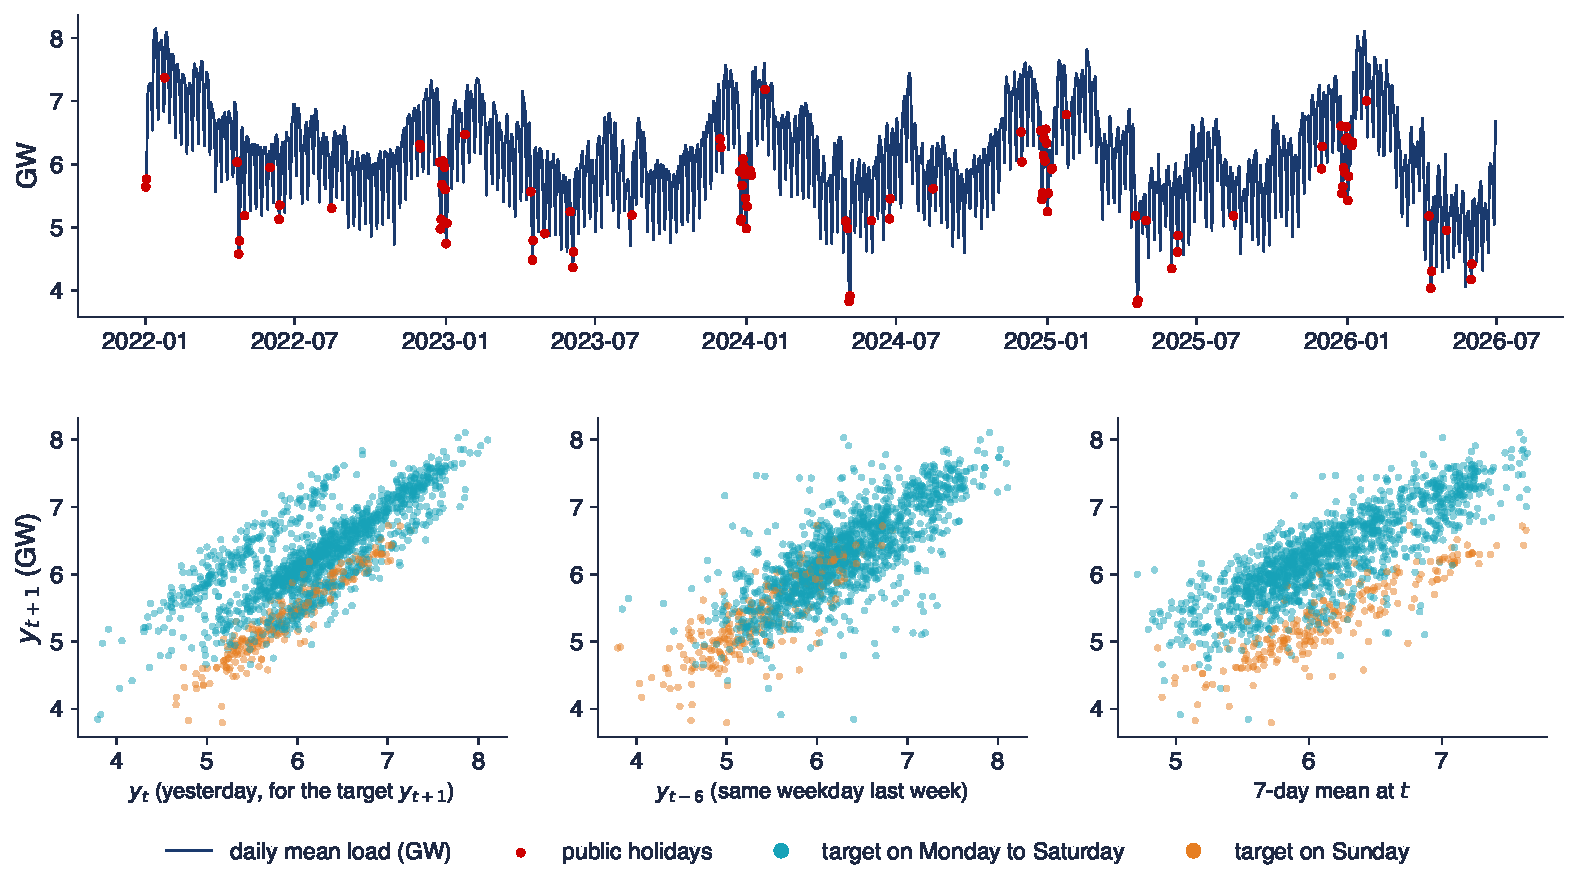
\includegraphics[width=0.97\textwidth,height=0.56\textheight,keepaspectratio]{tsa_ch9_features.pdf}
\end{center}
\vspace{-0.25cm}
\begin{itemize}
    \item Consumul mediu zilnic al României, ENTSO-E (rețeaua europeană a operatorilor de transport și de sistem pentru energie electrică), 1 ianuarie 2022--30 iunie 2026, 1\,642 de zile; jos: consumul de mîine față de trei variabile explicative
\end{itemize}
\quantlet{TSA\_ch9\_supervised\_learning}{\qlurl{TSA_ch9_supervised_learning}}
\end{frame}

\begin{frame}{Interpretarea variabilelor pentru consum}
\itemsize{\small}
\begin{itemize}
    \item Media 6{,}18 GW; minimul 3{,}79 GW pe 20 aprilie 2025 (Paștele ortodox), maximul 8{,}15 GW pe 13 ianuarie 2022 (o săptămînă de iarnă)
    \begin{itemize}
        \item ciclul săptămînal, ciclul anual (încălzire iarna, răcire vara) și scăderi mari de sărbători: sezonalitatea multiplă din \tsachlink{https://danpele.github.io/Time-Series-Analysis/RO/Cursuri/capitol4_sezonalitate_prognoza.pdf}{Capitolul 4}
    \end{itemize}
    \item Corelația cu consumul de mîine: $y_t$ 0{,}77; aceeași zi a săptămînii trecute 0{,}82; media pe 7 zile 0{,}74
    \begin{itemize}
        \item doar cu $y_t$, duminicile formează un nor separat: un singur lag liniar nu poate reprezenta tiparul săptămînal
        \item tabelul folosit mai departe are 1\,614 de rînduri și 30 de variabile explicative (14 laguri, două medii, aceeași zi a săptămînii, calendar)
    \end{itemize}
\end{itemize}
\end{frame}

\begin{frame}{Prognoze pe mai mulți pași: trei strategii}
\itemsize{\small}
\begin{itemize}
    \item \textbf{Recursivă} (iterată): un model pentru $h = 1$; prognoza lui înlocuiește valoarea necunoscută $y_{T+1}$ și modelul se aplică din nou
    \begin{itemize}
        \item așa prognozează ARIMA (\tsachlink{https://danpele.github.io/Time-Series-Analysis/RO/Cursuri/capitol3_radacini_unitare_modele_arima.pdf}{Capitolul 3}); erorile se acumulează cînd modelul pe un pas este greșit
    \end{itemize}
    \item \textbf{Directă}: un model separat $\hat f_h$ pentru fiecare orizont $h = 1, \dots, H$, antrenat pe ținta $y_{t+h}$
    \begin{itemize}
        \item erorile nu se acumulează, dar avem $H$ modele și mai puține rînduri pentru orizonturi lungi; prognozele pentru $h$ diferite pot fi incoerente
    \end{itemize}
    \item \textbf{Cu ieșiri multiple} (MIMO, multiple-input multiple-output): un model întoarce vectorul $(\hat y_{T+1}, \dots, \hat y_{T+H})$
    \begin{itemize}
        \item natural pentru rețelele neuronale; sinteză și comparație: \refBenTaieb
    \end{itemize}
\end{itemize}
\end{frame}

\begin{frame}{Prognoze recursive, directe și cu ieșiri multiple}
\itemsize{\footnotesize}
\begin{center}
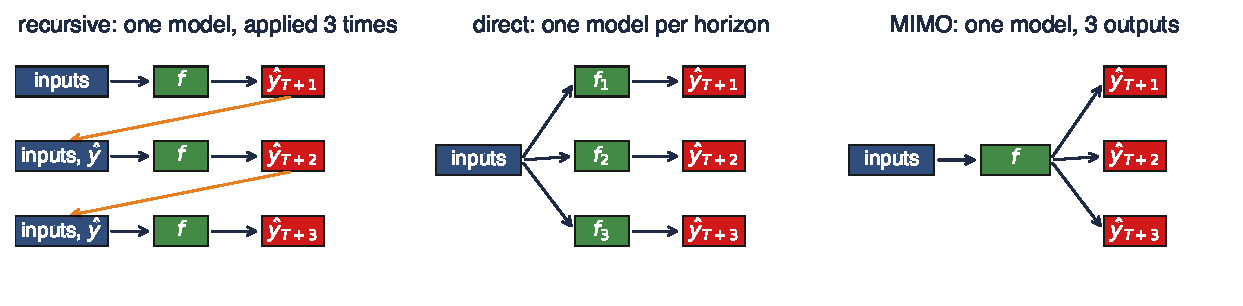
\includegraphics[width=0.97\textwidth,height=0.45\textheight,keepaspectratio]{tsa_ch9_strategies.pdf}
\end{center}
\vspace{-0.25cm}
\begin{itemize}
    \item Albastru: intrările cunoscute la originea $T$; verde: modelele estimate; roșu: prognozele; portocaliu: o prognoză folosită din nou ca intrare
\end{itemize}
\quantlet{TSA\_ch9\_supervised\_learning}{\qlurl{TSA_ch9_supervised_learning}}
\end{frame}

\begin{frame}{Exemplu rezolvat: prognoze recursive și directe pe doi pași}
\itemsize{\small}
\begin{itemize}
    \item Modelul pe un pas estimat pe tabel: $\hat y_{t+1} = 1{,}2 + 0{,}8\,y_t$; ultima valoare $y_T = 5$
    \begin{itemize}
        \item recursiv: $\hat y_{T+1} = 1{,}2 + 0{,}8 \cdot 5 = 5{,}20$; \quad $\hat y_{T+2} = 1{,}2 + 0{,}8 \cdot 5{,}20 = 5{,}36$
        \item regula implicită pe doi pași: $\hat y_{T+2} = 2{,}16 + 0{,}64\,y_T$
    \end{itemize}
    \item Modelul direct estimat pe ținta $y_{t+2}$: $\hat y_{t+2} = 2{,}3 + 0{,}6\,y_t$; \quad $\hat y_{T+2} = 5{,}30$
    \begin{itemize}
        \item dacă AR(1) ar fi modelul adevărat, coeficienții direcți ar estima aceleași valori, $2{,}16$ și $0{,}64$
        \item diferă: modelul pe un pas este greșit specificat la doi pași (de exemplu, un tipar săptămînal), iar modelul direct se adaptează orizontului
    \end{itemize}
    \item Nicio strategie nu este întotdeauna superioară: le încercăm pe amîndouă pe datele de validare
\end{itemize}
\end{frame}

\begin{frame}{Recapitulare: prognoza ca învățare supervizată}
\itemsize{\small}
\begin{itemize}
    \item O prognoză este o predicție a lui $y_{t+h}$ din variabile cunoscute la $t$: laguri, statistici pe ferestre mobile, calendar
    \item Un AR$(p)$ este o regresie liniară pe laguri; ML schimbă funcția, nu tabelul
    \item Pe mai mulți pași: recursiv (un model, iterat), direct (un model pentru fiecare $h$), MIMO (un model, $H$ ieșiri)
\end{itemize}
\end{frame}


%=============================================================================
\section{Validare fără leakage}
%=============================================================================

\begin{frame}{Eșantioanele de antrenare, validare și test}
\itemsize{\small}
\begin{itemize}
    \item Eșantionul de \textbf{antrenare}: estimează parametrii; de \textbf{validare}: alege hiperparametrii; de \textbf{test}: măsoară acuratețea finală, folosit o singură dată
    \begin{itemize}
        \item pentru serii de timp cele trei eșantioane sînt blocuri consecutive, în această ordine
    \end{itemize}
    \item Validarea \textbf{walk-forward} (validarea încrucișată pentru serii de timp, \tsachlink{https://danpele.github.io/Time-Series-Analysis/RO/Cursuri/capitol4_sezonalitate_prognoza.pdf}{Capitolul 4}): antrenăm pe datele de pînă la o origine, prognozăm blocul următor, mutăm originea înainte
    \begin{itemize}
        \item fereastră \textbf{extinsă}: toate datele trecute; fereastră \textbf{mobilă}: ultimele $W$ observații (se adaptează schimbărilor, folosește mai puține date)
        \item erorile tuturor originilor se combină în MAE, RMSE, MASE (\tsachlink{https://danpele.github.io/Time-Series-Analysis/RO/Cursuri/capitol0_introducere.pdf}{Capitolul 0}) și se compară cu testul Diebold--Mariano
    \end{itemize}
    \item Validarea încrucișată cu $K$ grupuri aleatoare este validă doar pentru autoregresii pure cu erori de tip zgomot alb \refBHK
\end{itemize}
\end{frame}

\begin{frame}{Patru scheme de validare}
\itemsize{\footnotesize}
\begin{center}
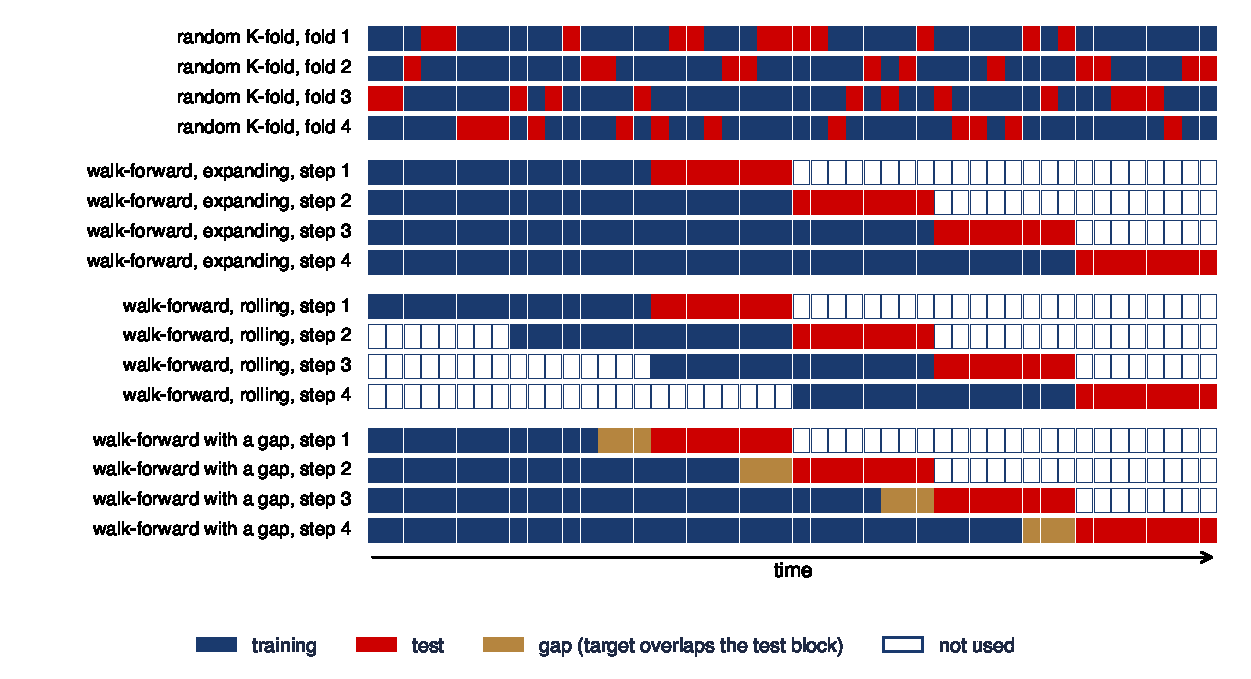
\includegraphics[width=0.97\textwidth,height=0.56\textheight,keepaspectratio]{tsa_ch9_cv_schemes.pdf}
\end{center}
\vspace{-0.25cm}
\begin{itemize}
    \item $K$-fold aleator amestecă trecutul și viitorul; walk-forward păstrează ordinea; un spațiu (gap) elimină rîndurile de antrenare ale căror ținte se suprapun cu blocul de test
\end{itemize}
\quantlet{TSA\_ch9\_validation}{\qlurl{TSA_ch9_validation}}
\end{frame}

\begin{frame}{Look-ahead bias și leakage-ul}
\itemsize{\small}
\begin{itemize}
    \item \textbf{Leakage-ul} (scurgerea de informație): informație care nu ar fi disponibilă la originea prognozei intră în antrenare sau în variabile \refKaufman
    \begin{itemize}
        \item rezultat: scoruri excelente la validare, care dispar la utilizarea reală; în finanțe se numește \textbf{look-ahead bias}
    \end{itemize}
    \item Surse tipice
    \begin{itemize}
        \item o medie mobilă sau o diferență care include $y_{t+1}$; mediile mobile centrate și filtrele bilaterale (\tsachlink{https://danpele.github.io/Time-Series-Analysis/RO/Cursuri/capitol0_introducere.pdf}{Capitolul 0})
        \item scalarea, completarea valorilor lipsă sau selecția variabilelor estimate pe tot eșantionul înainte de împărțire
        \item ținte suprapuse (sume pe următoarele $h$ zile) cu grupuri aleatoare sau fără spațiu (gap)
        \item date macroeconomice revizuite: versiunea de azi a PIB-ului nu era cunoscută la origine; vremea efectivă în locul prognozei meteo
    \end{itemize}
    \item Regula: scrieți codul variabilelor ca funcție doar de datele de pînă la $t$ și reestimați fiecare pas de preprocesare în fiecare fereastră de antrenare
\end{itemize}
\end{frame}

\begin{frame}{Leakage-ul în practică: grupuri aleatoare pe ținte suprapuse}
\itemsize{\footnotesize}
\begin{center}
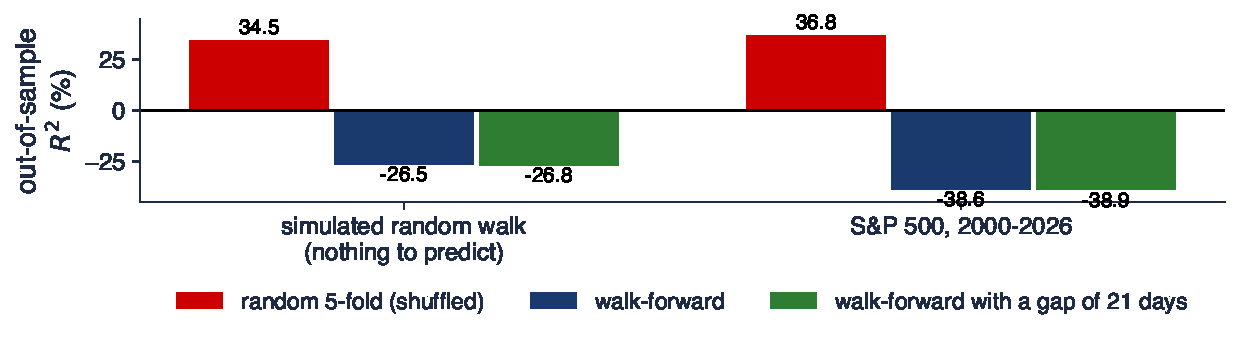
\includegraphics[width=0.97\textwidth,height=0.5\textheight,keepaspectratio]{tsa_ch9_leakage.pdf}
\end{center}
\vspace{-0.25cm}
\begin{itemize}
    \item Random forest pentru suma următoarelor 21 de randamente zilnice; variabile: sume trecute pe 5, 21, 63 de zile și volatilități; stînga: un mers aleator simulat; dreapta: S\&P 500, 6\,631 de zile
\end{itemize}
\quantlet{TSA\_ch9\_validation}{\qlurl{TSA_ch9_validation}}
\end{frame}

\begin{frame}{Interpretarea experimentului de leakage}
\itemsize{\small}
\begin{itemize}
    \item 5-fold aleator raportează $R^2$ = 34{,}5\% pentru un mers aleator, unde nimic nu este previzibil, și 36{,}8\% pentru S\&P 500
    \begin{itemize}
        \item țintele vecine au în comun 20 din 21 de randamente: un rînd de test are aproape-copii în grupurile de antrenare
    \end{itemize}
    \item Walk-forward: $-$26{,}5\% și $-$38{,}6\%; cu un spațiu de 21 de zile: $-$26{,}8\% și $-$38{,}9\%
    \begin{itemize}
        \item $R^2$ negativ în afara eșantionului: random forest este mai slab decît media istorică, cum ne așteptăm pentru randamente (\tsachlink{https://danpele.github.io/Time-Series-Analysis/RO/Cursuri/capitol1_procese_stochastice_stationaritate.pdf}{Capitolul 1})
    \end{itemize}
    \item Un model este atît de bun cît este validarea lui; un scor spectaculos este un motiv să căutăm un leakage
\end{itemize}
\end{frame}

\begin{frame}{Overfitting și compromisul deplasare--varianță}
\itemsize{\small}
\begin{itemize}
    \item Modelul $y = f(x) + \varepsilon$, $\Var(\varepsilon) = \sigma^2$; $\hat f$ estimat pe un eșantion de antrenare aleator
    \begin{itemize}
        \item eroarea de test așteptată într-un punct $x_0$:
        \item $E[(y_0 - \hat f(x_0))^2] = \underbrace{(E[\hat f(x_0)] - f(x_0))^2}_{\text{deplasare}^2} + \underbrace{\Var(\hat f(x_0))}_{\text{varianță}} + \sigma^2$
        \item $f$: funcția adevărată; $y_0$: o observație nouă în $x_0$; media se ia după eșantioanele de antrenare și zgomot; $\sigma^2$: zgomotul pe care niciun model nu îl poate elimina
    \end{itemize}
    \item \textbf{Overfitting}: un model flexibil învață zgomotul; eroare de antrenare mică, eroare de test mare
    \begin{itemize}
        \item \textbf{underfitting}: un model rigid ratează semnalul (deplasare mare)
    \end{itemize}
    \item Fiecare metodă ML are un parametru de complexitate (adîncime, număr de arbori, penalizare, neuroni ascunși); validarea îl fixează
\end{itemize}
\end{frame}

\begin{frame}{Deplasarea și varianța arborilor de regresie}
\itemsize{\footnotesize}
\begin{center}
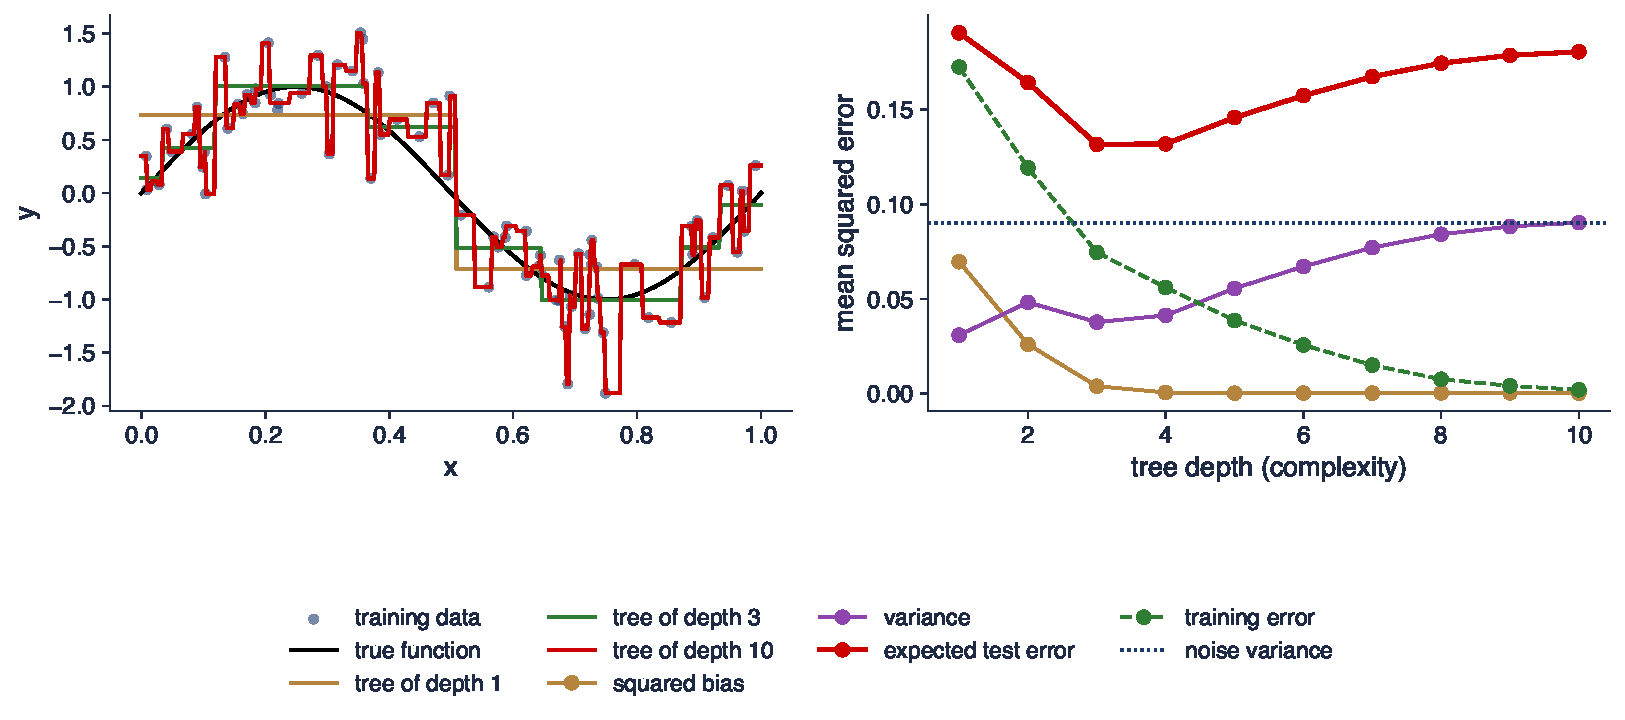
\includegraphics[width=0.97\textwidth,height=0.52\textheight,keepaspectratio]{tsa_ch9_bias_variance.pdf}
\end{center}
\vspace{-0.25cm}
\begin{itemize}
    \item Simulare: $y = \sin(2\pi x) + \varepsilon$, $\sigma = 0{,}3$, 80 de puncte, 300 de eșantioane de antrenare; arbori de adîncime 1 pînă la 10
\end{itemize}
\quantlet{TSA\_ch9\_validation}{\qlurl{TSA_ch9_validation}}
\end{frame}

\begin{frame}{Interpretarea erorii de test în formă de U}
\itemsize{\small}
\begin{itemize}
    \item Adîncimea 1: deplasare$^2$ 0{,}070, varianță 0{,}031; adîncimea 10: deplasare$^2$ 0{,}000, varianță 0{,}090
    \begin{itemize}
        \item eroarea de test așteptată este minimă la adîncimea 3 (0{,}132), peste varianța zgomotului, 0,09
    \end{itemize}
    \item Eroarea de antrenare scade la 0{,}002 la adîncimea 10: nu poate alege complexitatea
    \item Ansamblurile (random forest, boosting) și penalizările (ridge, lasso) reduc varianța fără să piardă mult în deplasare
\end{itemize}
\end{frame}

\begin{frame}{Recapitulare: validare fără leakage}
\itemsize{\small}
\begin{itemize}
    \item Walk-forward: antrenăm pe trecut, testăm pe blocul următor, mergem mai departe; grupuri aleatoare doar pentru autoregresii pure
    \item Leakage-ul: valori viitoare în variabile, preprocesare pe tot eșantionul, ținte suprapuse, date revizuite
    \item Eroarea de test = deplasare$^2$ + varianță + zgomot; validarea fixează complexitatea
\end{itemize}
\end{frame}


%=============================================================================
\section{Modele liniare regularizate: ridge și lasso}
%=============================================================================

\begin{frame}{Multe laguri, metoda celor mai mici pătrate instabilă}
\itemsize{\small}
\begin{itemize}
    \item Model liniar pe $p$ variabile standardizate: $\hat y = \beta_0 + \sum_j \beta_j x_j$; OLS (ordinary least squares, metoda celor mai mici pătrate) minimizează $\sum_t (y_t - \hat y_t)^2$
    \begin{itemize}
        \item lagurile vecine sînt puternic corelate: coeficienții OLS devin mari, de semne opuse și instabili de la o fereastră la alta
    \end{itemize}
    \item \textbf{Standardizăm} întîi: $x_j \to (x_j - \bar x_j)/s_j$, cu $\bar x_j$, $s_j$ doar din fereastra de antrenare
    \begin{itemize}
        \item altfel penalizarea tratează inegal variabilele măsurate în GW și variabilele binare
    \end{itemize}
    \item Ideea regularizării: acceptăm puțină deplasare în schimbul unei scăderi mari a varianței
\end{itemize}
\end{frame}

\begin{frame}{Ridge și lasso}
\itemsize{\footnotesize}
\begin{itemize}
    \item \textbf{Ridge} \refHoerlK: $\min_{\beta} \sum_t (y_t - \beta_0 - \mathbf{x}_t'\beta)^2 + \lambda\sum_j \beta_j^2$
    \begin{itemize}
        \item $\lambda \ge 0$: penalizarea ($\lambda = 0$: OLS); $\mathbf{X}$: matricea variabilelor standardizate; $\mathbf{y}$: țintele; $\mathbf{I}$: matricea identitate
        \item formă închisă $\hat\beta = (\mathbf{X}'\mathbf{X} + \lambda\mathbf{I})^{-1}\mathbf{X}'\mathbf{y}$; toți coeficienții se contractă spre 0, niciunul nu devine exact 0
    \end{itemize}
    \item \textbf{Lasso} \refTib\ (least absolute shrinkage and selection operator): penalizarea $\lambda\sum_j |\beta_j|$
    \begin{itemize}
        \item face unii coeficienți exact 0: selectează lagurile
    \end{itemize}
    \item \textbf{Exemplu rezolvat}, o singură variabilă standardizată, $S_{xy} = \sum x_ty_t = 90$, $S_{xx} = \sum x_t^2 = 100$
    \begin{itemize}
        \item OLS $90/100 = 0{,}90$; ridge, $\lambda = 50$: $90/150 = 0{,}60$; lasso, $\lambda = 40$: $(90 - 20)/100 = 0{,}70$; lasso, $\lambda \ge 180$: exact 0
        \item lasso într-o dimensiune: $\hat\beta = \mathrm{sign}(S_{xy})\max(|S_{xy}| - \lambda/2, 0)/S_{xx}$ (prag moale, soft thresholding)
    \end{itemize}
    \item $\lambda$ se alege prin validare walk-forward (\texttt{TimeSeriesSplit}), niciodată prin grupuri aleatoare
\end{itemize}
\end{frame}

\begin{frame}{Traiectoriile ridge și lasso pentru variabilele consumului}
\itemsize{\footnotesize}
\begin{center}
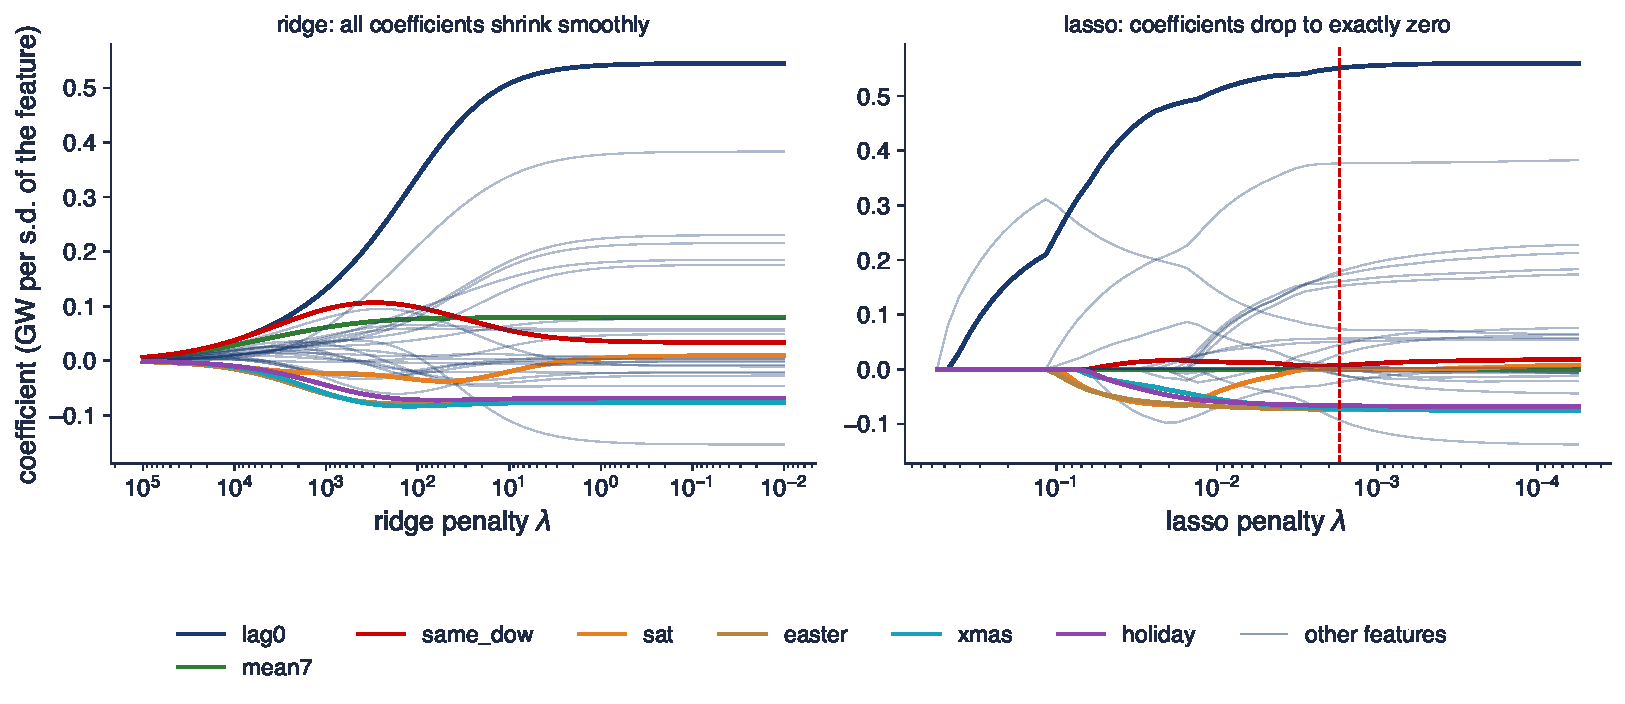
\includegraphics[width=0.97\textwidth,height=0.54\textheight,keepaspectratio]{tsa_ch9_shrinkage.pdf}
\end{center}
\vspace{-0.25cm}
\begin{itemize}
    \item Ținta: consumul de mîine; 30 de variabile standardizate; date pînă la 30 iunie 2025 (1\,249 de rînduri); linia întreruptă: penalizarea lasso aleasă prin validare walk-forward
\end{itemize}
\quantlet{TSA\_ch9\_regularisation\_trees}{\qlurl{TSA_ch9_regularisation_trees}}
\end{frame}

\begin{frame}{Interpretarea traiectoriilor coeficienților}
\itemsize{\small}
\begin{itemize}
    \item Cu o penalizare mare toți coeficienții sînt aproape de 0; cînd $\lambda$ scade, $y_t$ (lag0) intră primul și domină, cu coeficientul 0{,}55 GW la o abatere standard
    \begin{itemize}
        \item urmează variabilele binare ale zilelor și sărbătorile: calendarul poartă cea mai mare parte din semnalul rămas
    \end{itemize}
    \item La penalizarea aleasă, lasso păstrează 22 din 30 de variabile: multe laguri sînt redundante cînd $y_t$, ziua săptămînii și sărbătorile sînt incluse
    \item Ridge păstrează totul, dar contractă lin; pe originile de test din secțiunea 6, ridge este cel mai bun model ML
\end{itemize}
\end{frame}

\begin{frame}{Recapitulare: ridge și lasso}
\itemsize{\small}
\begin{itemize}
    \item Cele mai mici pătrate penalizate: ridge $\lambda\sum\beta_j^2$ contractă; lasso $\lambda\sum|\beta_j|$ contractă și selectează
    \item Standardizăm în fiecare fereastră de antrenare; alegem $\lambda$ prin walk-forward
    \item Un AR regularizat cu variabile de calendar este un reper ML puternic
\end{itemize}
\end{frame}


%=============================================================================
\section{Arbori, random forest și gradient boosting}
%=============================================================================

\begin{frame}{Arborii de regresie}
\itemsize{\small}
\begin{itemize}
    \item Un \textbf{arbore de regresie} împarte spațiul variabilelor prin întrebări „$x_j \le c$?” și prognozează, în fiecare regiune finală (frunză), media țintei din rîndurile de antrenare ale acesteia
    \begin{itemize}
        \item împărțirea se alege lacom (greedy): perechea $(j, c)$ cu cea mai mică sumă a pătratelor erorilor celor doi descendenți
    \end{itemize}
    \item Puncte tari: neliniaritate și interacțiuni (ziua săptămînii $\times$ sezon) fără să le specificăm; nu necesită scalare
    \begin{itemize}
        \item puncte slabe: un singur arbore este instabil (varianță mare) și constant pe porțiuni
    \end{itemize}
    \item \textbf{Un arbore nu poate extrapola}: prognoza lui este întotdeauna o medie a unor ținte din antrenare
    \begin{itemize}
        \item pentru serii cu trend: modelăm diferențe, rate de creștere sau abaterea de la trend, nu niveluri
    \end{itemize}
\end{itemize}
\end{frame}

\begin{frame}{Un arbore de adîncime 2 pentru consumul de mîine}
\itemsize{\footnotesize}
\begin{center}
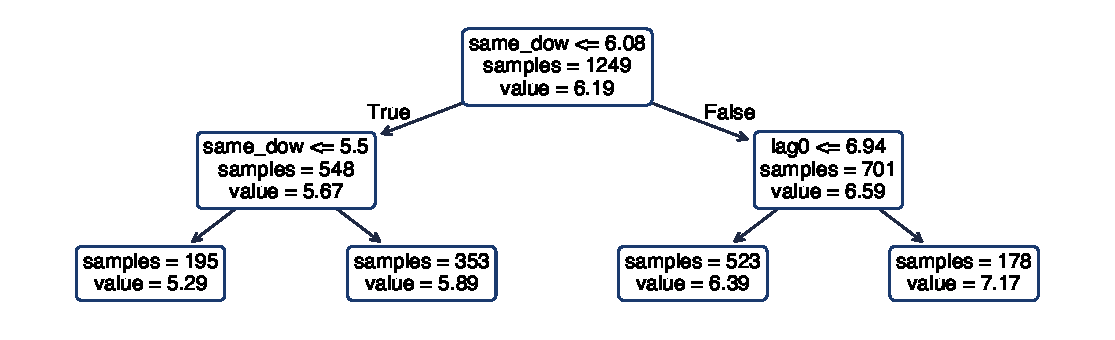
\includegraphics[width=0.97\textwidth,height=0.5\textheight,keepaspectratio]{tsa_ch9_tree.pdf}
\end{center}
\vspace{-0.25cm}
\begin{itemize}
    \item Variabile: $y_t$ (lag0), aceeași zi a săptămînii trecute (same\_dow), indicatori de weekend și de sărbătoare; date pînă la 30 iunie 2025; cel puțin 20 de zile în fiecare frunză
\end{itemize}
\quantlet{TSA\_ch9\_regularisation\_trees}{\qlurl{TSA_ch9_regularisation_trees}}
\end{frame}

\begin{frame}{Interpretarea arborelui}
\itemsize{\small}
\begin{itemize}
    \item Prima întrebare: a fost aceeași zi a săptămînii trecute sub 6{,}08 GW? Separă weekendurile și sărbătorile de zilele lucrătoare
    \begin{itemize}
        \item patru frunze: 5{,}29; 5{,}89; 6{,}39 și 7{,}17 GW, cu 195, 353, 523 și 178 de zile
    \end{itemize}
    \item Patru numere explică deja $R^2$ = 0{,}64 din varianță la antrenare; arborii mai adînci adaugă detalii și varianță
    \item Prognoza pentru orice zi este una dintre aceste patru medii: un arbore nu prognozează niciodată în afara intervalului țintelor de antrenare
\end{itemize}
\end{frame}

\begin{frame}{Random forest}
\itemsize{\small}
\begin{itemize}
    \item \textbf{Bagging} (bootstrap aggregation): creștem $B$ arbori adînci pe eșantioane bootstrap ale rîndurilor și facem media lor
    \begin{itemize}
        \item media a $B$ arbori cu corelația $\rho$ și varianța $\sigma^2$ are varianța $\rho\sigma^2 + (1 - \rho)\sigma^2/B$
    \end{itemize}
    \item \textbf{Random forest} \refBreiman: la fiecare împărțire se încearcă doar o submulțime aleatoare de variabile (\texttt{max\_features})
    \begin{itemize}
        \item astfel arborii se decorelează ($\rho$ scade), iar media are o varianță mai mică
    \end{itemize}
    \item Hiperparametri: numărul de arbori (un număr mai mare nu înrăutățește rezultatul, doar mărește timpul de calcul), \texttt{max\_features}, dimensiunea minimă a frunzei
    \begin{itemize}
        \item bootstrap-ul ignoră ordinea în timp în fereastra de antrenare; nu este o problemă, deoarece validarea este walk-forward
    \end{itemize}
\end{itemize}
\end{frame}

\begin{frame}{Gradient boosting}
\itemsize{\footnotesize}
\begin{itemize}
    \item \textbf{Boosting} \refFriedman: adăugăm cîte un arbore mic, fiecare estimat pe reziduurile (gradientul negativ al funcției de pierdere) modelului curent
    \begin{itemize}
        \item $F_m(\mathbf{x}) = F_{m-1}(\mathbf{x}) + \nu\,g_m(\mathbf{x})$; $F_m$: modelul după $m$ arbori; $g_m$: al $m$-lea arbore mic; $\nu$: \textbf{rata de învățare} (0,01--0,3)
    \end{itemize}
    \item \textbf{Exemplu rezolvat}: țintele $5, 6, 8$; pornim de la medie, $F_0 = 6{,}33$; reziduurile $-$1{,}33; $-$0{,}33; +1{,}67
    \begin{itemize}
        \item un arbore cu o singură împărțire care izolează al treilea punct prognozează acolo $1{,}67$; cu $\nu = 0{,}1$: $F_1 = 6{,}33 + 0{,}1 \cdot 1{,}67 = 6{,}500$
    \end{itemize}
    \item Implementările rapide grupează variabilele în histograme: XGBoost \refXGB, LightGBM \refLGBM, \texttt{HistGradientBoostingRegressor} în scikit-learn
    \begin{itemize}
        \item mai departe notăm GB pentru gradient boosting; cîștigătorii M5 (secțiunea 10) au folosit LightGBM
        \item hiperparametri: numărul de arbori cu \textbf{oprire timpurie} pe datele de validare, dimensiunea arborilor, $\nu$, dimensiunea minimă a frunzei
    \end{itemize}
\end{itemize}
\end{frame}

\begin{frame}{Un arbore, un random forest și boosting pe datele de consum}
\itemsize{\footnotesize}
\begin{center}
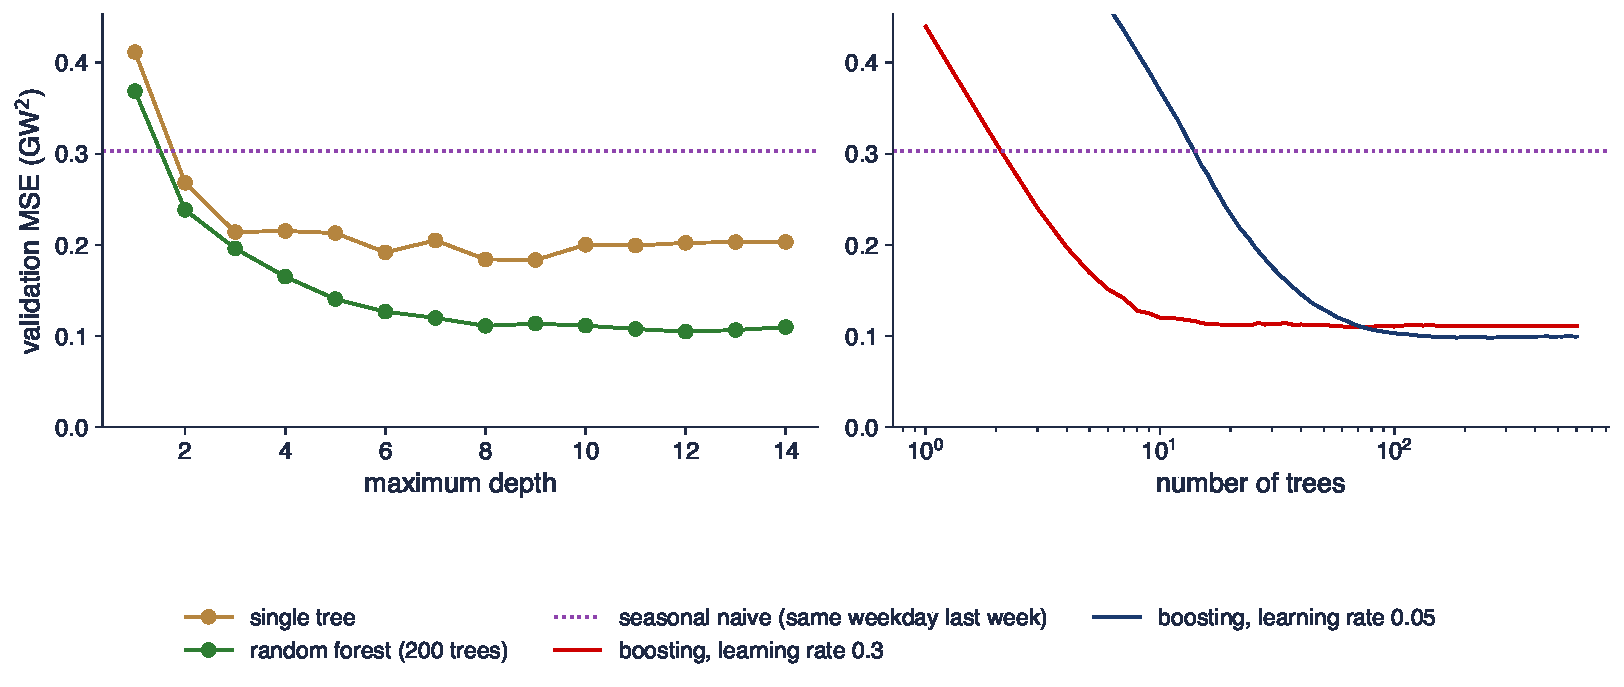
\includegraphics[width=0.97\textwidth,height=0.5\textheight,keepaspectratio]{tsa_ch9_ensembles.pdf}
\end{center}
\vspace{-0.25cm}
\begin{itemize}
    \item Consumul de mîine; antrenare pînă la 31 decembrie 2024 (1069 de zile), validare ianuarie--iunie 2025 (180 de zile); linia punctată: prognoza naivă sezonieră
\end{itemize}
\quantlet{TSA\_ch9\_regularisation\_trees}{\qlurl{TSA_ch9_regularisation_trees}}
\end{frame}

\begin{frame}{Interpretarea ansamblurilor}
\itemsize{\small}
\begin{itemize}
    \item Un singur arbore: cea mai bună MSE (mean squared error, eroarea pătratică medie) la validare, 0{,}183, la adîncimea 9; random forest: 0{,}105 la adîncimea 12
    \begin{itemize}
        \item media elimină cea mai mare parte a varianței; prognoza naivă sezonieră are 0{,}303
    \end{itemize}
    \item Boosting cu $\nu = 0{,}3$: minimul 0{,}110 după 72 de arbori; cu $\nu = 0{,}05$: 0{,}098 după 256 de arbori
    \begin{itemize}
        \item o rată de învățare mică are nevoie de mai mulți arbori și ajunge de obicei puțin mai jos; oprirea timpurie alege numărul de arbori
    \end{itemize}
\end{itemize}
\end{frame}

\begin{frame}{Arborii nu pot extrapola: nivelul prețurilor în România}
\itemsize{\footnotesize}
\begin{center}
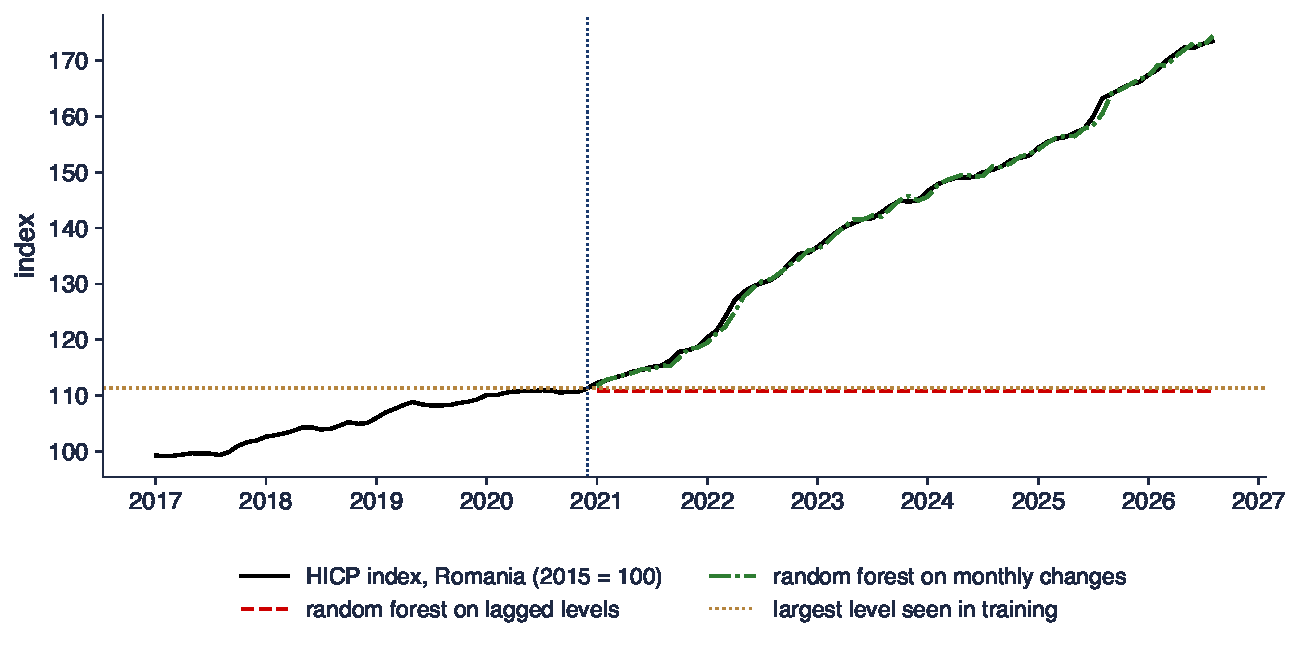
\includegraphics[width=0.97\textwidth,height=0.5\textheight,keepaspectratio]{tsa_ch9_extrapolation.pdf}
\end{center}
\vspace{-0.25cm}
\begin{itemize}
    \item IAPC (indicele armonizat al prețurilor de consum) al României, Eurostat, 2015 = 100; prognoze cu o lună înainte din random forest antrenate pînă în decembrie 2020, pe laguri ale nivelurilor sau pe variațiile lunare logaritmice
\end{itemize}
\quantlet{TSA\_ch9\_regularisation\_trees}{\qlurl{TSA_ch9_regularisation_trees}}
\end{frame}

\begin{frame}{Interpretarea eșecului de extrapolare}
\itemsize{\small}
\begin{itemize}
    \item Cel mai mare indice din antrenare a fost 111{,}3; în august 2026 indicele a ajuns la 173{,}4
    \begin{itemize}
        \item random forest pe niveluri rămîne în jurul valorii 110{,}8 timp de cinci ani: RMSE 36{,}9 puncte de indice
    \end{itemize}
    \item Același random forest pe variațiile lunare, apoi cumulate, urmărește indicele: RMSE 0{,}71
    \item Din nou \tsachlink{https://danpele.github.io/Time-Series-Analysis/RO/Cursuri/capitol3_radacini_unitare_modele_arima.pdf}{Capitolul 3}: diferențiem sau transformăm seriile nestaționare înainte ca un arbore să le vadă
\end{itemize}
\end{frame}

\begin{frame}{Variabilele folosite de model}
\itemsize{\small}
\begin{itemize}
    \item \textbf{Importanța prin permutare}: amestecăm o variabilă în datele de test și măsurăm cît crește eroarea
    \begin{itemize}
        \item nu depinde de tipul modelului; se măsoară în afara eșantionului; variabilele corelate își împart (și își ascund) importanța
    \end{itemize}
    \item Importanța calculată din impuritatea arborilor (MDI, mean decrease impurity) se obține la antrenare și favorizează variabilele continue: preferăm permutarea
    \item Importanța nu înseamnă cauzalitate: descrie modelul, nu sistemul energetic
\end{itemize}
\end{frame}

\begin{frame}{Importanța prin permutare pentru gradient boosting}
\itemsize{\footnotesize}
\begin{center}
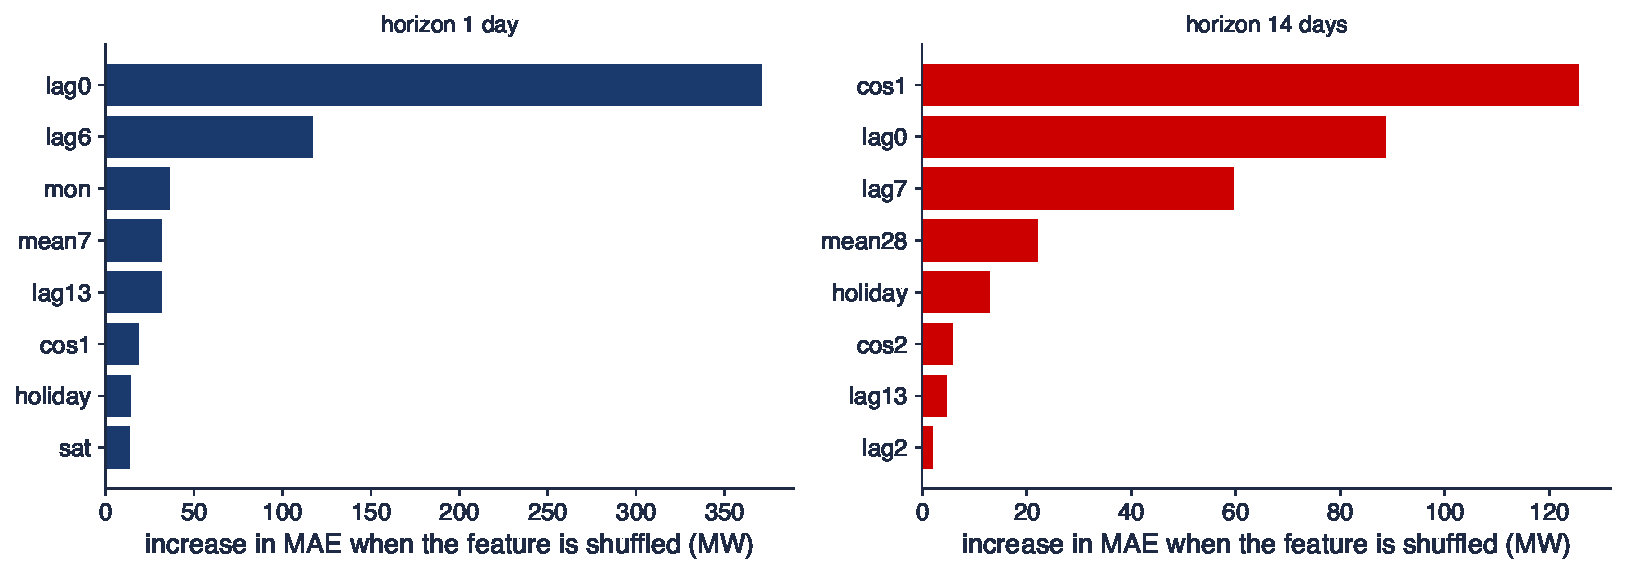
\includegraphics[width=0.97\textwidth,height=0.5\textheight,keepaspectratio]{tsa_ch9_importance.pdf}
\end{center}
\vspace{-0.25cm}
\begin{itemize}
    \item Modele GB directe pentru orizonturile de 1 și 14 zile; antrenate pînă la 31 decembrie 2024, evaluate pe ianuarie--iunie 2025; 20 de permutări aleatoare pentru fiecare variabilă
\end{itemize}
\quantlet{TSA\_ch9\_load\_forecasting}{\qlurl{TSA_ch9_load_forecasting}}
\end{frame}

\begin{frame}{Interpretarea importanțelor}
\itemsize{\small}
\begin{itemize}
    \item Cu o zi înainte: lag0 (+371 MW de MAE cînd este amestecată) și lag6 (+117 MW) domină
    \begin{itemize}
        \item ziua de ieri și aceeași zi a săptămînii trecute: persistența și ciclul săptămînal
    \end{itemize}
    \item Cu paisprezece zile înainte: cos1 (+126 MW) și lag0 (+89 MW)
    \begin{itemize}
        \item ciclul anual (cos1, termenul Fourier) cîștigă importanță pe măsură ce valorile recente devin mai puțin informative
    \end{itemize}
\end{itemize}
\end{frame}

\begin{frame}{Recapitulare: arbori și ansambluri}
\itemsize{\small}
\begin{itemize}
    \item Un arbore este o funcție constantă pe porțiuni, găsită prin împărțiri lacome; nu poate extrapola
    \item Random forest face media unor arbori adînci decorelați (mai puțină varianță); boosting adaugă arbori mici pe reziduuri (mai puțină deplasare)
    \item GB (gradient boosting, LightGBM, XGBoost, \texttt{HistGradientBoosting}): rata de învățare, numărul de arbori, oprirea timpurie
    \item Importanța prin permutare măsoară ce folosește modelul, în afara eșantionului
\end{itemize}
\end{frame}


%=============================================================================
\section{Rețele neuronale}
%=============================================================================

\begin{frame}{Perceptronul multistrat}
\itemsize{\footnotesize}
\begin{columns}[T]
\begin{column}{0.36\textwidth}
\centering
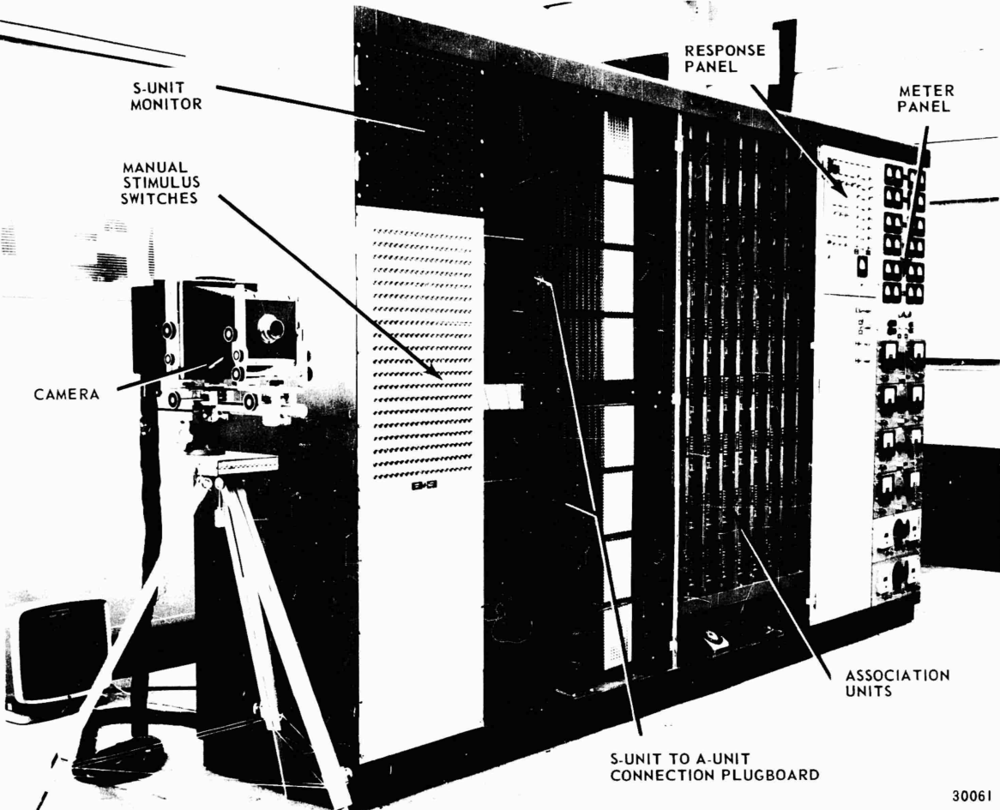
\includegraphics[height=0.5\textheight]{ch9_mark1_perceptron_1960.png}\\[1mm]
\imgcap{Mark I Perceptron, Cornell (1960): prima rețea neuronală antrenabilă, construită fizic}
\imgcredit{https://commons.wikimedia.org/wiki/File:Mark_I_Perceptron,_Figure_2_of_operator\%27s_manual.png}{Imagine: J. C. Hay, A. E. Murray (1960), Mark I Perceptron operator's manual; public domain; Wikimedia Commons}
\end{column}
\begin{column}{0.62\textwidth}
\begin{itemize}
    \item \textbf{MLP} (multilayer perceptron, perceptron multistrat), un strat ascuns cu $q$ neuroni:
    \begin{itemize}
        \item $h_j = g(b_j + \mathbf{w}_j'\mathbf{x})$, $j = 1, \dots, q$; \quad $\hat y = c + \sum_j v_jh_j$
        \item $\mathbf{x}$: intrările; $\mathbf{w}_j$, $b_j$: ponderile și termenul liber ale neuronului $j$; $h_j$: ieșirea lui; $v_j$, $c$: ponderile și termenul liber ale ieșirii
        \item $g$: funcția de activare (ReLU $\max(0, z)$, tanh, logistică); cu $g(z) = z$ rețeaua redevine liniară
    \end{itemize}
    \item Aproximarea universală \refHornik: suficienți neuroni ascunși aproximează orice funcție continuă
    \begin{itemize}
        \item parametri: 3 intrări și 5 neuroni dau deja $3 \cdot 5 + 5 + 5 + 1 = 26$ de ponderi
    \end{itemize}
\end{itemize}
\end{column}
\end{columns}
\end{frame}

\begin{frame}{O rețea mică și funcțiile ei de activare}
\itemsize{\footnotesize}
\begin{center}
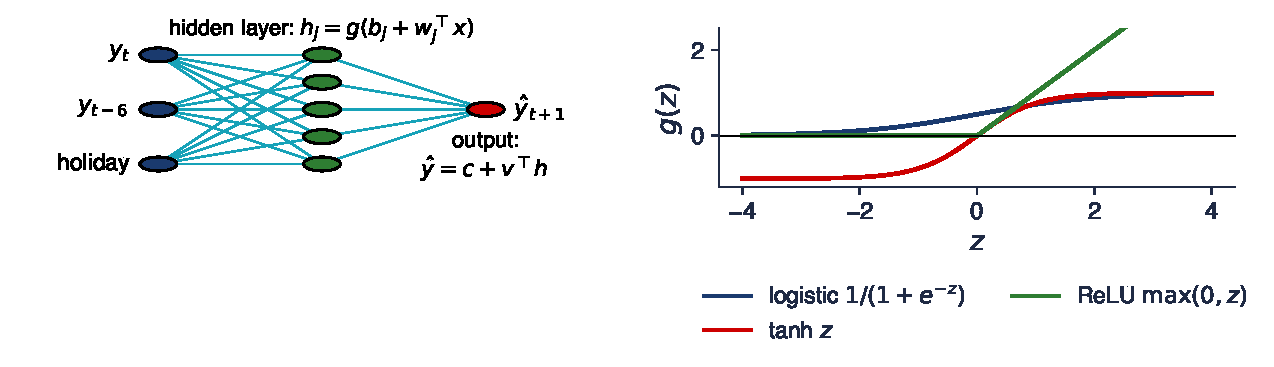
\includegraphics[width=0.97\textwidth,height=0.48\textheight,keepaspectratio]{tsa_ch9_mlp.pdf}
\end{center}
\vspace{-0.25cm}
\begin{itemize}
    \item Stînga: 3 intrări (ziua de ieri, aceeași zi a săptămînii trecute, indicatorul de sărbătoare), 5 neuroni ascunși, o ieșire; dreapta: trei funcții de activare
\end{itemize}
\quantlet{TSA\_ch9\_neural\_networks}{\qlurl{TSA_ch9_neural_networks}}
\end{frame}

\begin{frame}{Antrenarea unei rețele}
\itemsize{\small}
\begin{itemize}
    \item Minimizăm pierderea la antrenare prin \textbf{coborîre pe gradient}; gradienții se obțin prin retropropagare (back-propagation) \refRumelhart
    \begin{itemize}
        \item SGD (stochastic gradient descent) și Adam folosesc loturi mici aleatoare; o trecere prin date este o epocă
    \end{itemize}
    \item Suprafața pierderii are multe minime locale: rezultatele depind de ponderile inițiale aleatoare
    \begin{itemize}
        \item fixăm sămînța și facem media cîtorva rețele cu semințe diferite (un ansamblu)
    \end{itemize}
    \item Regularizare: o penalizare L2 pe ponderi, oprirea timpurie, dropout (dezactivarea aleatoare a unor neuroni)
    \begin{itemize}
        \item intrările și țintele trebuie standardizate cu statisticile ferestrei de antrenare
    \end{itemize}
    \item Datele puține (cîteva mii de rînduri) favorizează rețelele mici; rețelele adînci au nevoie de multe serii sau de date lungi, de frecvență înaltă
\end{itemize}
\end{frame}

\begin{frame}{Rețele recurente și LSTM (1/2): rețeaua recurentă}
\itemsize{\footnotesize}
\begin{itemize}
    \item \textbf{RNN} (recurrent neural network, rețea neuronală recurentă): o stare ascunsă duce trecutul mai departe, cu aceleași ponderi la fiecare pas
    \begin{itemize}
        \item $h_t = \tanh(Wh_{t-1} + Ux_t + b)$: noua stare combină starea anterioară și noua intrare
        \item $x_t$: intrarea la momentul $t$; $h_t$: starea ascunsă; $W$, $U$, $b$: ponderile și termenul liber, comune tuturor pașilor; $\tanh$ ține fiecare componentă în $(-1, 1)$
        \item prognoza se citește din ultima stare, de exemplu $\hat y_{t+1} = v'h_t + c$
    \end{itemize}
    \item Dificultatea: antrenarea prin mulți pași înmulțește multe derivate
    \begin{itemize}
        \item gradienții dispar sau explodează: un RNN simplu uită ce s-a întîmplat cu mai mult de cîțiva pași în urmă
    \end{itemize}
    \item Concluzia sintezei \refHBB
    \begin{itemize}
        \item pe serii unice și scurte, rețelele recurente sînt rareori mai precise decît ETS sau ARIMA
        \item sînt utile mai ales cu multe serii înrudite și suficiente date (modele globale, \refDeepAR)
    \end{itemize}
\end{itemize}
\end{frame}

\begin{frame}{Rețele recurente și LSTM (2/2): celula LSTM}
\itemsize{\footnotesize}
\begin{itemize}
    \item \textbf{LSTM} (long short-term memory) \refLSTM: o stare a celulei $c_t$ actualizată aditiv, controlată de trei porți
    \begin{itemize}
        \item porțile: $f_t = \sigma(W_f[h_{t-1}, x_t] + b_f)$ (uitare), $i_t = \sigma(W_i[h_{t-1}, x_t] + b_i)$ (intrare), $o_t = \sigma(W_o[h_{t-1}, x_t] + b_o)$ (ieșire)
        \item conținutul nou propus: $\tilde c_t = \tanh(W_c[h_{t-1}, x_t] + b_c)$
        \item $\sigma(z) = 1/(1 + e^{-z}) \in (0, 1)$: funcția logistică; $[h_{t-1}, x_t]$: cei doi vectori puși unul sub altul; $W_f, W_i, W_o, W_c$ și $b_f, b_i, b_o, b_c$: ponderile și termenii liberi
    \end{itemize}
    \item Actualizarea celulei și a ieșirii
    \begin{itemize}
        \item $c_t = f_t \odot c_{t-1} + i_t \odot \tilde c_t$: cu $f_t$ apropiat de 1 memoria veche se păstrează pe mulți pași; $i_t$ stabilește cît conținut nou intră
        \item $h_t = o_t \odot \tanh(c_t)$: poarta de ieșire decide ce parte a memoriei este transmisă mai departe; $\odot$: produsul element cu element
    \end{itemize}
    \item Fiecare poartă este un mic strat logistic: un LSTM cu 32 de unități și 8 intrări are circa 5\,400 de ponderi
\end{itemize}
\end{frame}

\begin{frame}{O rețea recurentă și celula LSTM}
\itemsize{\footnotesize}
\begin{center}
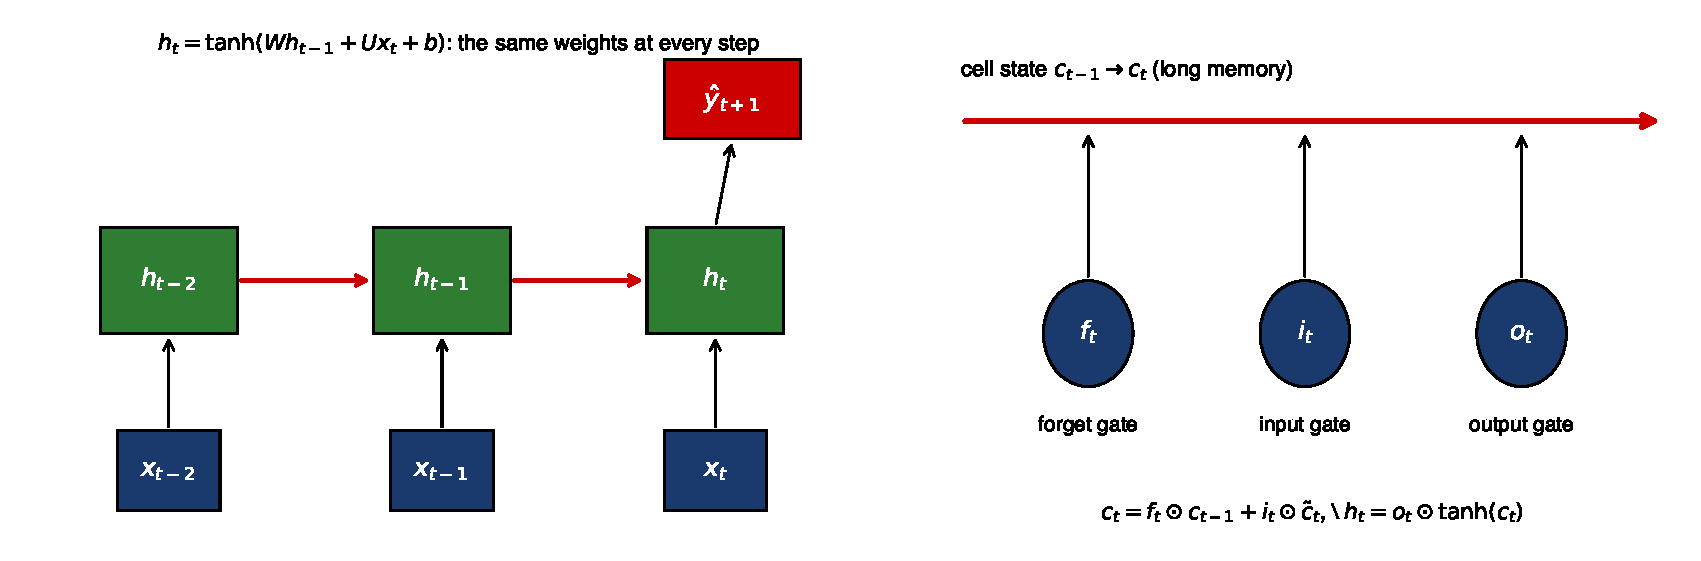
\includegraphics[width=0.97\textwidth,height=0.48\textheight,keepaspectratio]{tsa_ch9_rnn.pdf}
\end{center}
\vspace{-0.25cm}
\begin{itemize}
    \item Stînga: RNN desfășurată pe trei pași; dreapta: starea celulei LSTM (roșu) și cele trei porți; $\odot$: produsul element cu element
\end{itemize}
\quantlet{TSA\_ch9\_neural\_networks}{\qlurl{TSA_ch9_neural_networks}}
\end{frame}

\begin{frame}{Sepp Hochreiter și LSTM}
\itemsize{\small}
\begin{columns}[T]
\begin{column}{0.38\textwidth}
\centering

\includegraphics[height=0.55\textheight]{ch9_sepp_hochreiter_2015.jpg}\\[1mm]
\imgcap{Sepp Hochreiter (2015), Universitatea Johannes Kepler din Linz}
\imgcredit{https://commons.wikimedia.org/wiki/File:Sepp_Hochreiter.JPG}{Foto: Eulenreich (2015); CC BY-SA 4.0; Wikimedia Commons}
\end{column}
\begin{column}{0.6\textwidth}
\begin{itemize}
    \item În lucrarea de diplomă din 1991, la München, Hochreiter a analizat de ce gradienții dispar în rețelele recurente
    \item Împreună cu Jürgen Schmidhuber a propus LSTM \refLSTM
    \begin{itemize}
        \item una dintre cele mai citate lucrări despre rețele neuronale
    \end{itemize}
    \item LSTM a stat la baza recunoașterii vorbirii și a traducerii automate înainte de transformer (\tsachlink{https://danpele.github.io/Time-Series-Analysis/RO/Cursuri/capitol11_foundation_models_serii_timp.pdf}{Capitolul 11})
\end{itemize}
\end{column}
\end{columns}
\end{frame}

\begin{frame}{Recapitulare: rețele neuronale}
\itemsize{\small}
\begin{itemize}
    \item MLP: straturi de $g(b + \mathbf{w}'\mathbf{x})$; antrenat prin coborîre pe gradient; sămînța, scalarea, penalizarea L2, oprirea timpurie
    \item RNN și LSTM procesează secvențe; starea celulei LSTM evită dispariția gradienților
    \item Datele puține favorizează modelele mici; rețelele neuronale au nevoie de multe serii sau de date lungi
\end{itemize}
\end{frame}


%=============================================================================
\section{Aplicație: consumul de energie electrică și Capitolul 4}
%=============================================================================

\begin{frame}{Exercițiul de prognoză}
\itemsize{\footnotesize}
\begin{columns}[T]
\begin{column}{0.34\textwidth}
\centering
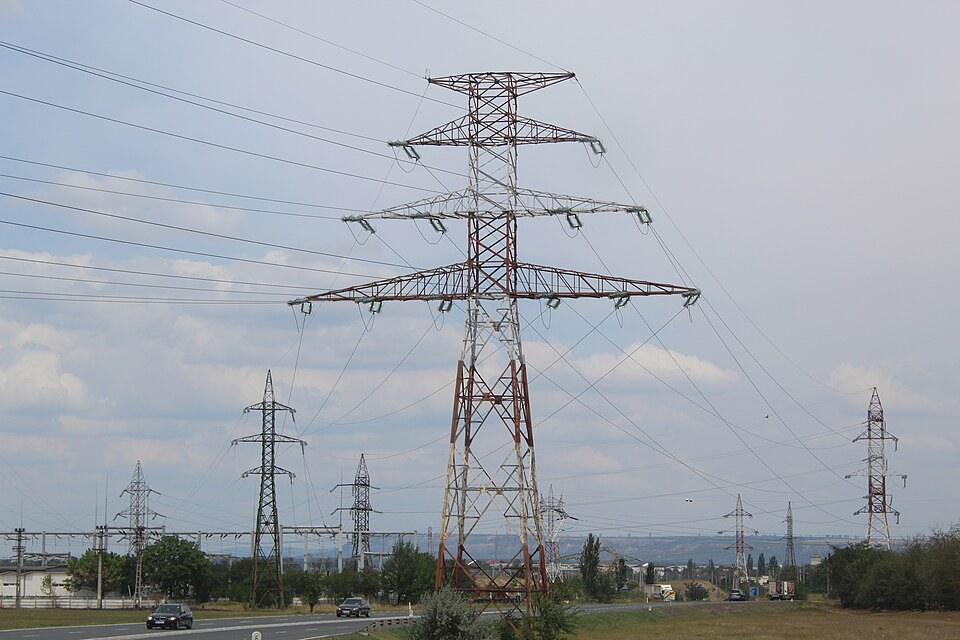
\includegraphics[height=0.45\textheight]{ch9_marasesti_750kv_2022.jpg}\\[1mm]
\imgcap{Linia de 750 kV de la Mărășești: rețeaua de transport a României}
\imgcredit{https://commons.wikimedia.org/wiki/File:750_kV_electricity_tower_at_M\%C4\%83r\%C4\%83\%C8\%99e\%C8\%99ti,_Romania.jpg}{Foto: TrainSimFan (2022); CC BY-SA 4.0; Wikimedia Commons}
\end{column}
\begin{column}{0.64\textwidth}
\begin{itemize}
    \item Schema de evaluare din \tsachlink{https://danpele.github.io/Time-Series-Analysis/RO/Cursuri/capitol4_sezonalitate_prognoza.pdf}{Capitolul 4}: 26 de origini ale prognozei, la fiecare 14 zile, de la 30 iunie 2025 la 15 iunie 2026
    \begin{itemize}
        \item orizontul 1--14 zile; fereastră extinsă de la 1 ianuarie 2022
        \item modele statistice (\tsachlink{https://danpele.github.io/Time-Series-Analysis/RO/Cursuri/capitol4_sezonalitate_prognoza.pdf}{Capitolul 4}): naivă sezonieră, ETS, SARIMA, DHR (regresie armonică dinamică), combinația lor
    \end{itemize}
    \item Modele ML, reestimate la fiecare origine:
    \begin{itemize}
        \item directe: ridge, random forest (200 de arbori), GB (300 de arbori, $\nu = 0{,}05$), un model pentru fiecare orizont
        \item recursiv: GB pe tabelul pe un pas; MIMO: un MLP (3 rețele, 32 de neuroni) și un LSTM (56 de zile la intrare, 14 la ieșire)
    \end{itemize}
    \item Scala MASE: MAE în eșantion a metodei naive sezoniere săptămînale, 309 MW
\end{itemize}
\end{column}
\end{columns}
\end{frame}

\begin{frame}{Rezultatele: 26 de origini, 14 orizonturi}
\itemsize{\footnotesize}
\begin{center}
\scriptsize
\begin{tabular}{lrrrr}
\toprule
\textbf{Model} & MAE (GW) & RMSE (GW) & MASE & DM p, față de DHR \\
\midrule
Naivă sezonieră & 0{,}396 & 0{,}529 & 1{,}28 & $<$\,0{,}001 \\
ETS & 0{,}381 & 0{,}492 & 1{,}23 & 0{,}015 \\
SARIMA & 0{,}384 & 0{,}477 & 1{,}24 & 0{,}003 \\
DHR & 0{,}276 & 0{,}350 & 0{,}89 & -- \\
Combinația & 0{,}305 & 0{,}380 & 0{,}99 & 0{,}065 \\
Ridge & 0{,}277 & 0{,}337 & 0{,}90 & 0{,}942 \\
RF & 0{,}308 & 0{,}388 & 1{,}00 & 0{,}068 \\
GB direct & 0{,}298 & 0{,}369 & 0{,}97 & 0{,}163 \\
GB recursiv & 0{,}307 & 0{,}388 & 0{,}99 & 0{,}113 \\
MLP & 0{,}294 & 0{,}362 & 0{,}95 & 0{,}546 \\
LSTM & 0{,}357 & 0{,}447 & 1{,}16 & 0{,}016 \\
\bottomrule
\end{tabular}
\end{center}
\begin{itemize}
    \item DM: testul Diebold--Mariano pe erorile absolute medii pe origine (26 de valori), cu corecția Harvey--Leybourne--Newbold \refHLN
\end{itemize}
\end{frame}

\begin{frame}{MASE și acuratețea pe orizonturi}
\itemsize{\footnotesize}
\begin{center}
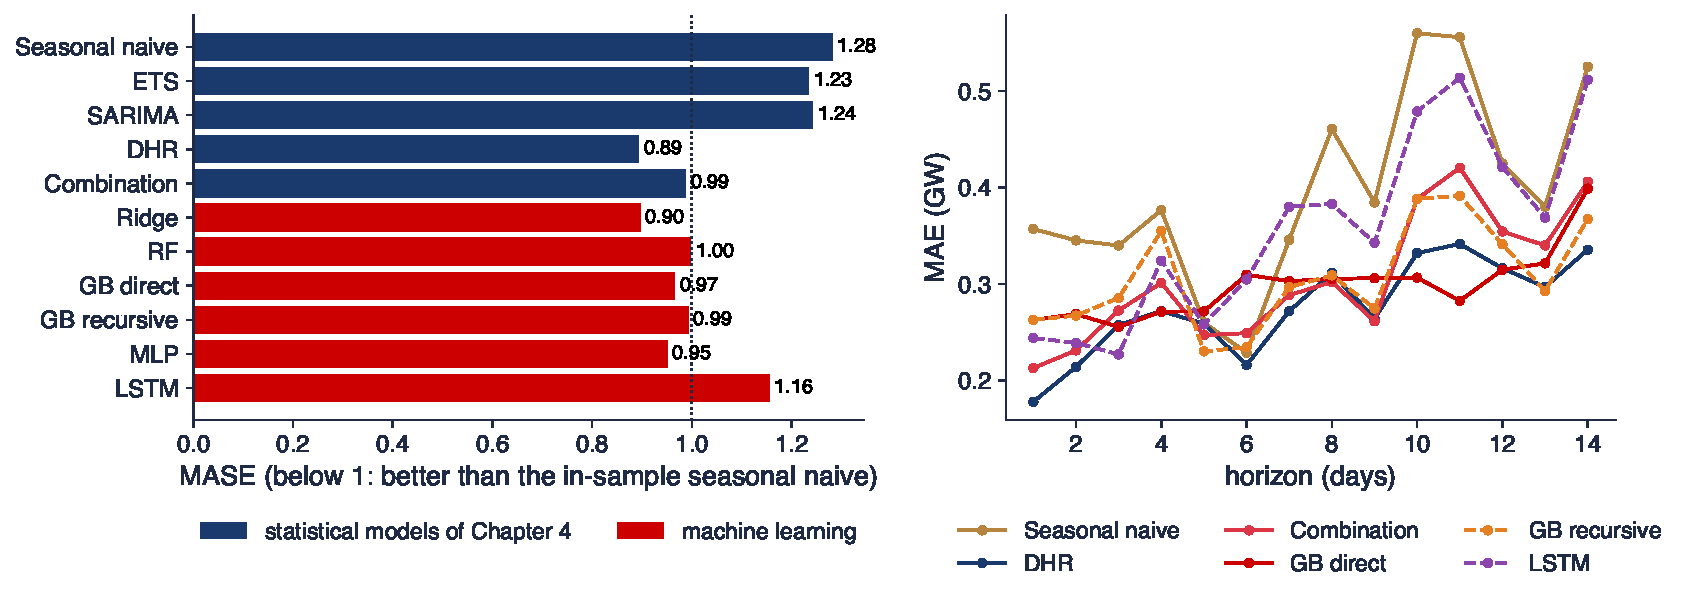
\includegraphics[width=0.97\textwidth,height=0.5\textheight,keepaspectratio]{tsa_ch9_load_results.pdf}
\end{center}
\vspace{-0.25cm}
\begin{itemize}
    \item Stînga: MASE pentru cele unsprezece modele (albastru: \tsachlink{https://danpele.github.io/Time-Series-Analysis/RO/Cursuri/capitol4_sezonalitate_prognoza.pdf}{Capitolul 4}; roșu: ML); dreapta: MAE pe orizonturi pentru șase modele
\end{itemize}
\quantlet{TSA\_ch9\_load\_forecasting}{\qlurl{TSA_ch9_load_forecasting}}
\end{frame}

\begin{frame}{Interpretarea rezultatelor pentru consum}
\itemsize{\small}
\begin{itemize}
    \item DHR (MASE 0{,}89) și ridge (0{,}90) sînt cele mai precise; diferența nu este semnificativă (p = 0{,}942)
    \begin{itemize}
        \item ambele sînt modele liniare cu variabilele de calendar potrivite; arborii și rețelele nu le depășesc
    \end{itemize}
    \item GB direct (0{,}97), MLP (0{,}95), random forest (1{,}00) depășesc clar metoda naivă sezonieră (p = 0{,}001), SARIMA și ETS
    \begin{itemize}
        \item GB direct și recursiv sînt apropiate (0{,}97 și 0{,}99); LSTM (1{,}16) este mai slab decît toate modelele, cu excepția celui naiv, SARIMA și ETS
    \end{itemize}
    \item Lecția: variabilele contează mai mult decît algoritmul; cu patru ani de date zilnice, un model liniar bine specificat este greu de depășit
\end{itemize}
\end{frame}

\begin{frame}{Prognozele în jurul Paștelui ortodox din 2026}
\itemsize{\footnotesize}
\begin{center}
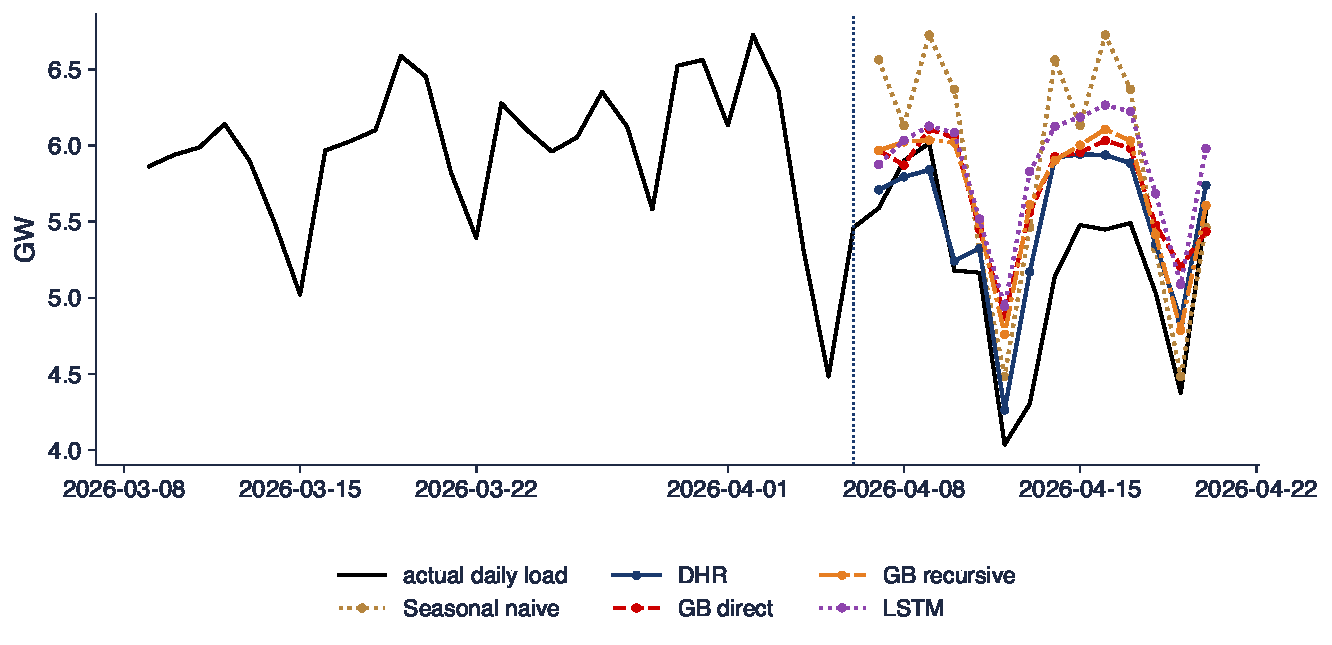
\includegraphics[width=0.97\textwidth,height=0.5\textheight,keepaspectratio]{tsa_ch9_load_forecasts.pdf}
\end{center}
\vspace{-0.25cm}
\begin{itemize}
    \item Originea 6 aprilie 2026; prognoze pe 14 zile; MAE în această fereastră: DHR 344 MW, GB direct 536 MW, GB recursiv 503 MW, LSTM 661 MW
\end{itemize}
\quantlet{TSA\_ch9\_load\_forecasting}{\qlurl{TSA_ch9_load_forecasting}}
\end{frame}

\begin{frame}{Interpretarea ferestrei de Paște}
\itemsize{\small}
\begin{itemize}
    \item Toate modelele văd indicatorul de Paște, dar arborii au doar patru sărbători de Paște la antrenare: prognozează o scădere prea mică
    \begin{itemize}
        \item DHR estimează un singur coeficient pentru Paște din aceleași patru episoade și folosește informația mai eficient
    \end{itemize}
    \item LSTM nu vede indicatorul de sărbătoare: repetă tiparul săptămînal și nu surprinde deloc sărbătoarea
    \item Evenimentele rare cer fie structură (un coeficient de regresie), fie multe serii care au în comun evenimentul (un model global)
\end{itemize}
\end{frame}

\begin{frame}{Recapitulare: consumul de energie electrică}
\itemsize{\small}
\begin{itemize}
    \item Aceleași origini, același orizont, aceleași erori: modelele ML intră în comparația din \tsachlink{https://danpele.github.io/Time-Series-Analysis/RO/Cursuri/capitol4_sezonalitate_prognoza.pdf}{Capitolul 4}
    \item Ridge are aceeași precizie ca DHR; GB, random forest și MLP depășesc SARIMA și ETS; LSTM nu
    \item Variabilele de calendar și sărbătorile decid clasamentul
\end{itemize}
\end{frame}


%=============================================================================
\section{Intervale de prognoză}
%=============================================================================

\begin{frame}{Regresia cuantilică și funcția de pierdere pinball}
\itemsize{\footnotesize}
\begin{itemize}
    \item O prognoză punctuală nu ajunge: operatorul rețelei are nevoie de consumul pe care nu îl va depăși cu probabilitatea de 95\%
    \begin{itemize}
        \item cuantila $\tau$, $q_\tau$, a lui $y_{t+h}$: $P(y_{t+h} \le q_\tau) = \tau$; un interval de 90\%: $[q_{0{,}05}, q_{0{,}95}]$
    \end{itemize}
    \item \textbf{Funcția de pierdere pinball}: $L_\tau(y, q) = \tau(y - q)$ dacă $y \ge q$ și $(1 - \tau)(q - y)$ dacă $y < q$ \refKB
    \begin{itemize}
        \item valoarea ei așteptată este minimă în cuantila adevărată; pentru $\tau = 0{,}5$ este jumătate din eroarea absolută
        \item exemplu, $\tau = 0{,}95$, $q = 7{,}0$ GW: $y = 7{,}4$ costă $0{,}95 \cdot 0{,}4 = 0{,}380$; $y = 6{,}5$ costă $0{,}05 \cdot 0{,}5 = 0{,}025$
    \end{itemize}
    \item Orice algoritm poate minimiza funcția pinball: regresia cuantilică liniară, GB cuantilic (\texttt{loss='quantile'}), rețelele
\end{itemize}
\end{frame}

\begin{frame}{Predicția conformală prin împărțire}
\itemsize{\footnotesize}
\begin{itemize}
    \item \textbf{Ideea} \refLei: folosim erorile modelului pe date pe care nu le-a văzut pentru a fixa lățimea intervalului
    \begin{itemize}
        \item 1. estimăm modelul pe datele de antrenare fără ultimele $n$ puncte (setul de calibrare)
        \item 2. calculăm erorile absolute $|e_i|$ pe setul de calibrare și le ordonăm
        \item 3. $\hat q$ = a $\lceil (n+1)(1 - \alpha) \rceil$-a cea mai mică valoare; intervalul $\hat y \pm \hat q$
        \item $\alpha$: proporția admisă de valori în afara intervalului ($\alpha = 0{,}1$ pentru un interval de 90\%); $\lceil\cdot\rceil$: rotunjirea în sus
    \end{itemize}
    \item Garanția: acoperire de cel puțin $1 - \alpha$ dacă erorile sînt interschimbabile (ordinea lor nu contează)
    \begin{itemize}
        \item seriile de timp nu sînt interschimbabile: garanția este aproximativă; folosim date de calibrare recente și reverificăm acoperirea prin walk-forward
    \end{itemize}
    \item Aici: $n = 182$ de zile, $\alpha = 0{,}1$, $\hat q$ = a 165-a cea mai mică eroare absolută, cîte un set de calibrare pentru fiecare orizont și origine
\end{itemize}
\end{frame}

\begin{frame}{Intervale de 90\% pentru consum}
\itemsize{\footnotesize}
\begin{center}
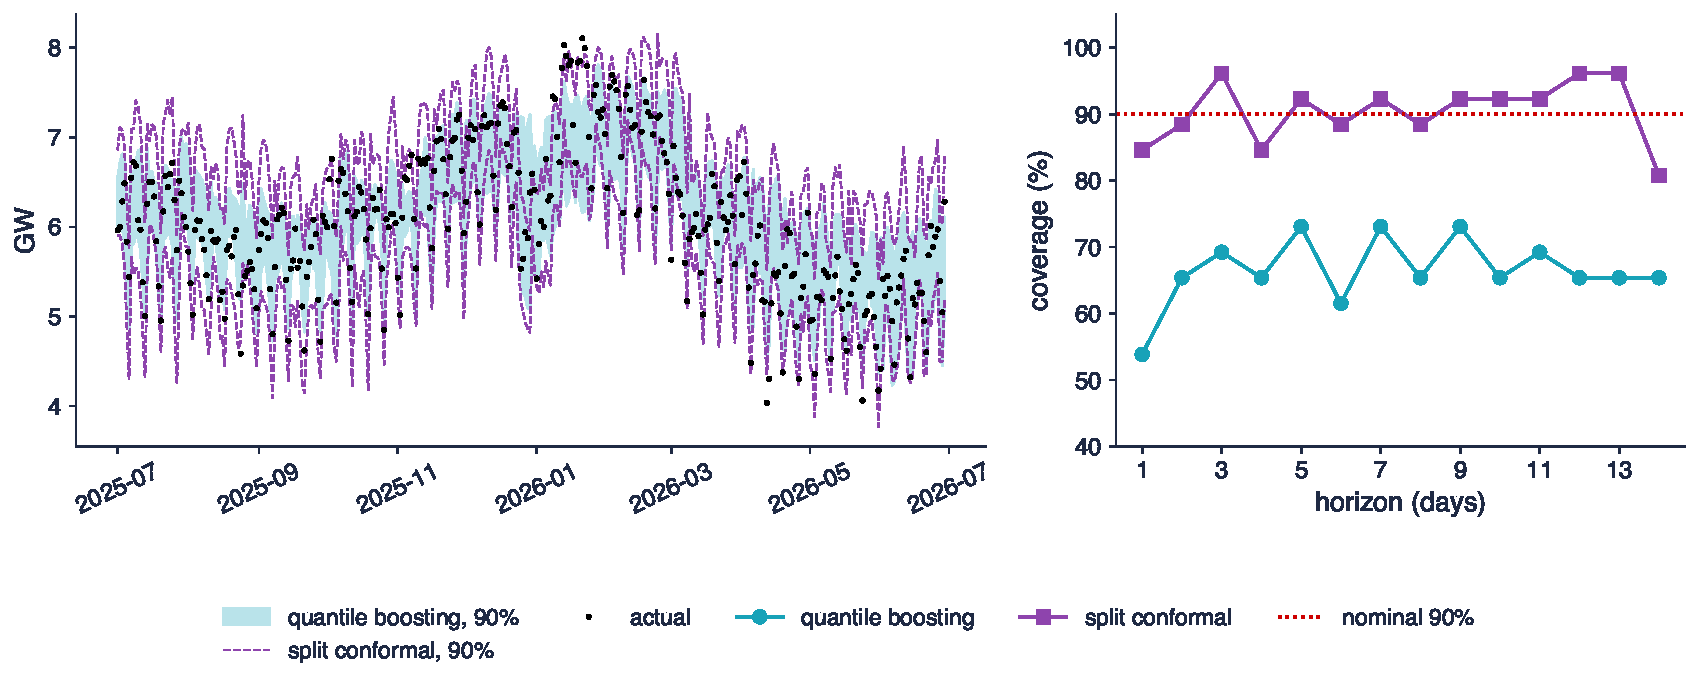
\includegraphics[width=0.97\textwidth,height=0.5\textheight,keepaspectratio]{tsa_ch9_intervals.pdf}
\end{center}
\vspace{-0.25cm}
\begin{itemize}
    \item GB direct, cele 364 de prognoze din secțiunea 6 (toate originile și orizonturile); stînga: intervale și valori realizate; dreapta: acoperirea pe orizonturi
\end{itemize}
\quantlet{TSA\_ch9\_load\_forecasting}{\qlurl{TSA_ch9_load_forecasting}}
\end{frame}

\begin{frame}{Interpretarea intervalelor}
\itemsize{\small}
\begin{itemize}
    \item GB cuantilic acoperă 66{,}5\%, cu lățimea medie de 884 MW; predicția conformală acoperă 90{,}4\%, cu lățimea de 1310 MW
    \begin{itemize}
        \item GB cuantilic: 19{,}0\% dintre valori sub interval și 14{,}6\% deasupra (nominal 5\% și 5\%)
    \end{itemize}
    \item Cuantilele estimate prin arbori sînt zgomotoase în cozi și prea înguste; calibrarea conformală corectează lățimea cu erori reale din afara eșantionului
    \item Raportați întotdeauna acoperirea empirică alături de un interval
\end{itemize}
\end{frame}

\begin{frame}{Recapitulare: intervale de prognoză}
\itemsize{\small}
\begin{itemize}
    \item Prognozele cuantilice minimizează funcția pinball; un interval este o pereche de cuantile
    \item Predicția conformală: $\hat y \pm$ o cuantilă empirică a erorilor de calibrare
    \item Verificăm acoperirea prin walk-forward
\end{itemize}
\end{frame}


%=============================================================================
\section{Modele locale și globale: inflația din România}
%=============================================================================

\begin{frame}{Modele locale și globale}
\itemsize{\small}
\begin{itemize}
    \item Model \textbf{local}: un model pentru fiecare serie, estimat doar pe acea serie (ARIMA, ETS, modelele de pînă acum)
    \begin{itemize}
        \item puținele observații ale unei serii limitează complexitatea pe care și-o poate permite un model local
    \end{itemize}
    \item Model \textbf{global}: un singur model estimat pe rîndurile combinate ale mai multor serii înrudite \refMMH, \refJanus
    \begin{itemize}
        \item aceleași variabile pentru fiecare serie (laguri scalate, calendar); opțional, un identificator al seriei
        \item mai multe date pentru fiecare parametru: algoritmii complecși (GB, rețele) devin utilizabili; cîștigătorii M4 și M5 au fost globali
    \end{itemize}
    \item Riscul: seriile trebuie să aibă dinamici comune; un model global poate face să dispară prin mediere ceea ce este specific unei serii
\end{itemize}
\end{frame}

\begin{frame}{Exercițiul pentru inflație}
\itemsize{\footnotesize}
\begin{itemize}
    \item Ținta: inflația anuală IAPC a României (Eurostat), $\pi_t = 100(P_t/P_{t-12} - 1)$, $P_t$: indicele IAPC, la orizonturile $h = 1, 3, 6, 12$ luni
    \begin{itemize}
        \item strategie directă; modelele prognozează variația $\pi_{t+h} - \pi_t$, deci arborii nu extrapolează niciodată nivelul
    \end{itemize}
    \item Variabile la $t$: $\pi_t, \pi_{t-1}, \pi_{t-2}, \pi_{t-3}, \pi_{t-6}, \pi_{t-12}$, ultimele trei variații lunare logaritmice și sumele lor pe 3 și 6 luni, luna calendaristică
    \begin{itemize}
        \item modele: mers aleator (RW, $\hat\pi_{t+h} = \pi_t$), AR (OLS pe aceleași variabile), lasso, random forest, GB local (doar România), GB global (27 de țări UE combinate)
    \end{itemize}
    \item Walk-forward: reestimare în fiecare ianuarie pe toate rîndurile a căror lună-țintă este deja observată (din 2006); originile de test ianuarie 2016--iulie 2026
    \item Rezultate înrudite: \refMedeiros\ arată că random forest depășește metodele de referință pentru inflația SUA cu peste 100 de predictori
\end{itemize}
\end{frame}

\begin{frame}{Inflația din România: prognoze și RMSE relativ}
\itemsize{\footnotesize}
\begin{center}
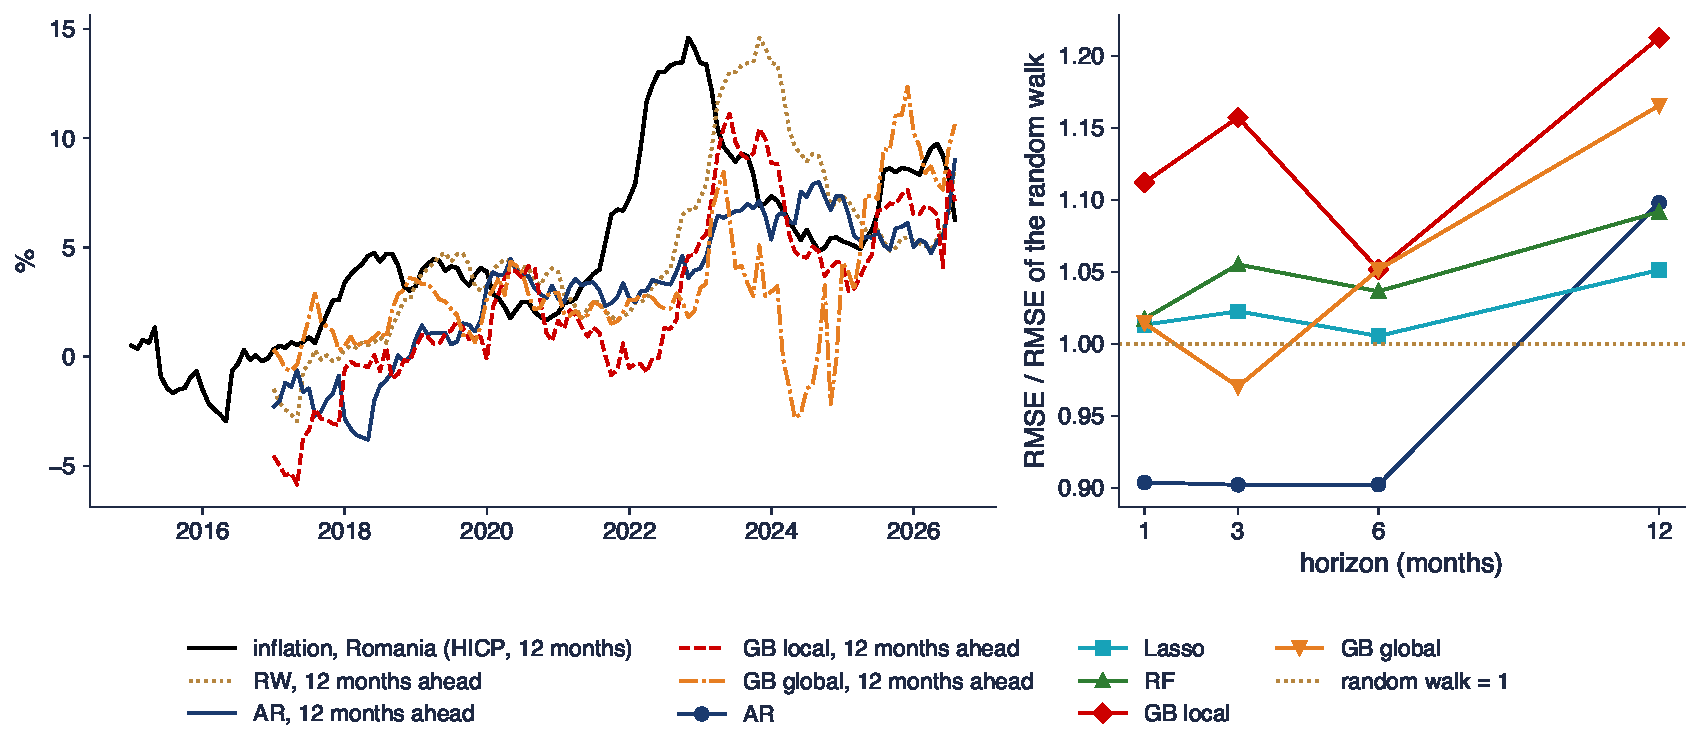
\includegraphics[width=0.97\textwidth,height=0.52\textheight,keepaspectratio]{tsa_ch9_inflation.pdf}
\end{center}
\vspace{-0.25cm}
\begin{itemize}
    \item Stînga: inflația și prognozele cu 12 luni înainte, reprezentate la luna-țintă; dreapta: RMSE relativ la mersul aleator
\end{itemize}
\quantlet{TSA\_ch9\_inflation\_global}{\qlurl{TSA_ch9_inflation_global}}
\end{frame}

\begin{frame}{Rezultatele pentru inflație}
\itemsize{\footnotesize}
\begin{center}
\scriptsize
\begin{tabular}{lrrrr}
\toprule
\textbf{RMSE (pp), relativ la RW} & $h = 1$ & $h = 3$ & $h = 6$ & $h = 12$ \\
\midrule
RW (mers aleator) & 0{,}63 (1{,}00) & 1{,}41 (1{,}00) & 2{,}25 (1{,}00) & 3{,}90 (1{,}00) \\
AR & 0{,}57 (0{,}90) & 1{,}28 (0{,}90) & 2{,}03 (0{,}90) & 4{,}28 (1{,}10) \\
Lasso & 0{,}64 (1{,}01) & 1{,}45 (1{,}02) & 2{,}26 (1{,}01) & 4{,}10 (1{,}05) \\
RF & 0{,}64 (1{,}02) & 1{,}49 (1{,}06) & 2{,}33 (1{,}04) & 4{,}25 (1{,}09) \\
GB local & 0{,}70 (1{,}11) & 1{,}64 (1{,}16) & 2{,}37 (1{,}05) & 4{,}72 (1{,}21) \\
GB global & 0{,}64 (1{,}01) & 1{,}37 (0{,}97) & 2{,}37 (1{,}05) & 4{,}54 (1{,}17) \\
\bottomrule
\end{tabular}
\end{center}
\begin{itemize}
    \item DM p față de RW, AR: 0{,}019 ($h = 1$), 0{,}186 ($h = 3$), 0{,}388 ($h = 6$); GB global față de GB local: 0{,}117; 0{,}113; 0{,}999; 0{,}828
    \item Origini de test: de la 127 ($h = 1$) la 116 ($h = 12$) luni; DM cu erori pătratice și $h - 1$ autocovarianțe
\end{itemize}
\end{frame}

\begin{frame}{Interpretarea rezultatelor pentru inflație}
\itemsize{\small}
\begin{itemize}
    \item AR liniar este cel mai bun model pînă la 6 luni (cu circa 10\% sub mersul aleator); niciun model ML nu depășește semnificativ mersul aleator
    \begin{itemize}
        \item la 12 luni niciun model nu depășește mersul aleator: vîrful din 2022 (14{,}6\% în noiembrie 2022) a venit din prețurile energiei, nu din trecutul inflației
    \end{itemize}
    \item GB global este mai bun decît cel local la orizonturi scurte (RMSE 1{,}37 față de 1{,}64 la $h = 3$), dar nesemnificativ (p = 0{,}113)
    \begin{itemize}
        \item combinarea a 27 de țări dă arborilor suficiente rînduri; GB local, cu 120--240 de rînduri la fiecare reestimare, face overfitting
    \end{itemize}
    \item Circa 120 de erori lunare de test nu pot separa modele ale căror RMSE diferă cu 5\%: concluzia onestă este „nu avem dovezi”
\end{itemize}
\end{frame}

\begin{frame}{Recapitulare: modele locale și globale}
\itemsize{\small}
\begin{itemize}
    \item Un model global combină multe serii înrudite și permite algoritmilor flexibili să folosească mai multe date
    \item Inflația din România: AR este cel mai bun; GB global depășește GB local; niciun model nu depășește mersul aleator la 12 luni
    \item Eșantioane mici: raportăm p-value-urile DM, nu doar clasamentele RMSE
\end{itemize}
\end{frame}


%=============================================================================
\section{Aplicații în finanțe: volatilitatea și semnul randamentului}
%=============================================================================

\begin{frame}{Volatilitatea realizată: HAR și ML (1/2)}
\itemsize{\footnotesize}
\begin{itemize}
    \item Ținta: logaritmul varianței zilnice medii pe următoarele 5 zile; aproximarea varianței zilnice din prețurile de deschidere, maxim, minim și închidere \refGK
    \begin{itemize}
        \item $\hat\sigma_t^2 = [\ln(O_t/C_{t-1})]^2 + \frac12[\ln(H_t/L_t)]^2 - (2\ln 2 - 1)[\ln(C_t/O_t)]^2$: pătratul randamentului de peste noapte plus termenul Garman--Klass
        \item $O_t$, $H_t$, $L_t$, $C_t$: prețurile de deschidere, maxim, minim și închidere din ziua $t$
        \item volatilitatea este persistentă și previzibilă (\tsachlink{https://danpele.github.io/Time-Series-Analysis/RO/Cursuri/capitol5_volatilitate_conditionata_garch.pdf}{Capitolul 5}): terenul potrivit pentru ML
    \end{itemize}
    \item Modelul \textbf{HAR} (heterogeneous autoregressive) \refCorsi: OLS pe logaritmul varianței din ultima zi, săptămînă și lună
    \begin{itemize}
        \item $\ln \bar\sigma^2_{t+1:t+5} = c + \beta_d \ln\hat\sigma_t^2 + \beta_w \ln\bar\sigma^2_{t-4:t} + \beta_m \ln\bar\sigma^2_{t-21:t} + u_t$; $\bar\sigma^2_{a:b}$: media lui $\hat\sigma^2$ în zilele de la $a$ la $b$; $u_t$: eroarea
        \item modelele ML adaugă 8 variabile: laguri ale varianței zilnice, media trimestrială, randamentul, partea lui negativă și valoarea lui absolută
    \end{itemize}
\end{itemize}
\end{frame}

\begin{frame}{Volatilitatea realizată: HAR și ML (2/2)}
\itemsize{\footnotesize}
\begin{itemize}
    \item Walk-forward anual din 2013, cu un spațiu de 5 zile între antrenare și test
    \item $R^2$ în afara eșantionului față de HAR: $R^2_{\text{HAR}} = 1 - \sum_t (y_t - \hat y_t)^2 / \sum_t (y_t - \hat y_t^{\text{HAR}})^2$
    \begin{itemize}
        \item $y_t$: logaritmul varianței realizate; $\hat y_t$, $\hat y_t^{\text{HAR}}$: prognozele modelului și ale HAR; pozitiv: mai precis decît HAR
    \end{itemize}
    \item QLIKE \refPatton: $L(\sigma^2, h) = \sigma^2/h + \ln h$, funcția de pierdere quasi-likelihood pentru varianță (\tsachlink{https://danpele.github.io/Time-Series-Analysis/RO/Cursuri/capitol5_volatilitate_conditionata_garch.pdf}{Capitolul 5}); o valoare mai mică este mai bună
    \begin{itemize}
        \item $\sigma^2$: varianța realizată; $h$: prognoza varianței; pentru un $\sigma^2$ dat, pierderea este minimă la $h = \sigma^2$ și penalizează mai mult prognozele prea mici
        \item robustă la zgomotul aproximării varianței: ordonează prognozele la fel ca varianța adevărată
    \end{itemize}
    \item Testul Diebold--Mariano (\tsachlink{https://danpele.github.io/Time-Series-Analysis/RO/Cursuri/capitol4_sezonalitate_prognoza.pdf}{Capitolul 4}) pe diferențele zilnice ale QLIKE
\end{itemize}
\end{frame}

\begin{frame}{Rezultatele: S\&P 500 și DAX, 2013--2026}
\itemsize{\footnotesize}
\begin{center}
\scriptsize
\begin{tabular}{lrrrrrr}
\toprule
\textbf{Model} & S\&P: $R^2$ față de HAR (\%) & QLIKE & DM $t$ & DAX: $R^2$ față de HAR (\%) & QLIKE & DM $t$ \\
\midrule
HAR & +0{,}0 & 0{,}414 & -- & +0{,}0 & 1{,}023 & -- \\
Lasso & +7{,}1 & 0{,}400 & $-$5{,}12 & +7{,}9 & 1{,}015 & $-$2{,}42 \\
RF & +1{,}0 & 0{,}416 & 0{,}32 & +3{,}5 & 1{,}024 & 0{,}03 \\
GB & $-$0{,}5 & 0{,}416 & 0{,}35 & +1{,}1 & 1{,}028 & 0{,}75 \\
MLP & +8{,}3 & 0{,}398 & $-$3{,}96 & +8{,}6 & 1{,}015 & $-$1{,}69 \\
\bottomrule
\end{tabular}
\end{center}
\begin{itemize}
    \item 3\,444 și 3\,473 de zile de test; DM $t < -1{,}96$: modelul are un QLIKE semnificativ mai mic decît HAR
    \item Lasso și MLP obțin un $R^2$ față de HAR de 7--9\% și reduc semnificativ QLIKE pe S\&P 500; random forest și GB nu depășesc HAR
    \item Cîștigul vine din variabilele suplimentare (randamentul negativ: efectul de levier din \tsachlink{https://danpele.github.io/Time-Series-Analysis/RO/Cursuri/capitol5_volatilitate_conditionata_garch.pdf}{Capitolul 5}), folosite lin; arborii taie o relație netedă în trepte
\end{itemize}
\end{frame}

\begin{frame}{Prognozele volatilității în două episoade de criză}
\itemsize{\footnotesize}
\begin{center}
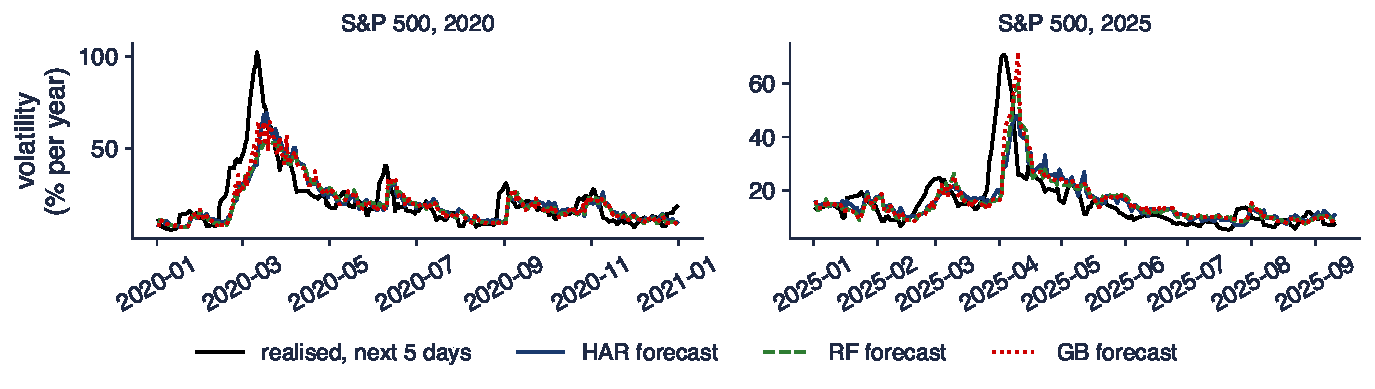
\includegraphics[width=0.97\textwidth,height=0.52\textheight,keepaspectratio]{tsa_ch9_rv.pdf}
\end{center}
\vspace{-0.25cm}
\begin{itemize}
    \item S\&P 500: volatilitatea realizată anualizată a următoarelor 5 zile și prognozele HAR, random forest și GB, 2020 și 2025
\end{itemize}
\quantlet{TSA\_ch9\_finance}{\qlurl{TSA_ch9_finance}}
\end{frame}

\begin{frame}{Semnul randamentului de mîine: reperul corect}
\itemsize{\footnotesize}
\begin{itemize}
    \item Clasificare: ținta $1\{r_{t+1} > 0\}$ (1 dacă randamentul de mîine este pozitiv, altfel 0); variabile: ultimele cinci randamente, sume pe 5, 21, 63 de zile, volatilitatea pe 21 și 63 de zile
    \begin{itemize}
        \item modele: regresia logistică (logit), random forest, GB; walk-forward anual din 2008
    \end{itemize}
    \item \textbf{Reperul corect} nu este 50\%: piețele cresc în mai multe zile decît scad
    \begin{itemize}
        \item „întotdeauna în creștere” (clasa majoritară din antrenare) are dreptate în 54{,}4\% din zilele S\&P 500 și în 53{,}8\% din zilele BET
    \end{itemize}
    \item Acuratețea, S\&P 500: logit 53{,}8\%, random forest 53{,}1\%, GB 52{,}5\%; BET: 53{,}7\%, 53{,}6\%, 52{,}2\%
    \item Niciun model nu depășește reperul; AUC (aria de sub curba ROC) 0{,}511--0{,}533, aproape de 0,5: nici capacitate de ordonare
    \begin{itemize}
        \item AUC: probabilitatea ca o zi de creștere aleasă la întîmplare să primească un scor mai mare decît o zi de scădere aleasă la întîmplare; 0,5: fără putere, 1: ordonare perfectă
    \end{itemize}
\end{itemize}
\end{frame}

\begin{frame}{Acuratețea față de reper}
\itemsize{\footnotesize}
\begin{center}
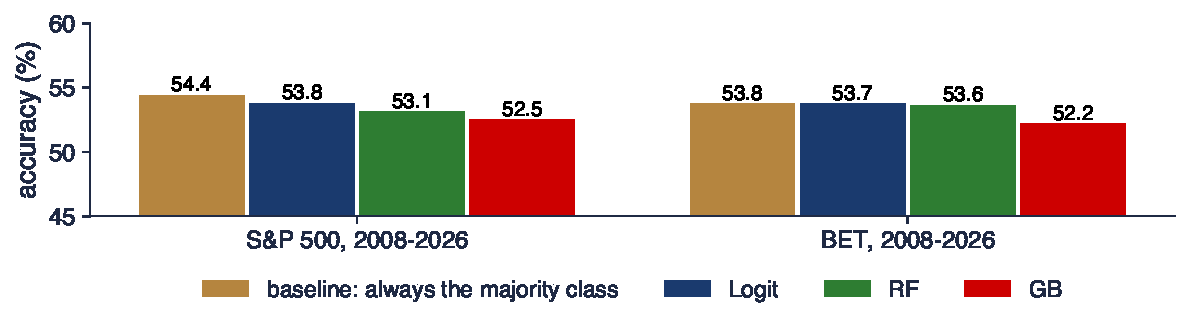
\includegraphics[width=0.97\textwidth,height=0.48\textheight,keepaspectratio]{tsa_ch9_sign.pdf}
\end{center}
\vspace{-0.25cm}
\begin{itemize}
    \item Acuratețea în afara eșantionului, 2008--2026: 4\,705 de zile S\&P 500 și 4\,686 de zile BET
\end{itemize}
\quantlet{TSA\_ch9\_finance}{\qlurl{TSA_ch9_finance}}
\end{frame}

\begin{frame}{Interpretarea experimentului privind semnul}
\itemsize{\small}
\begin{itemize}
    \item Un model cu „53\% acuratețe” pare performant; față de 54{,}4\% pentru „întotdeauna în creștere”, este mai slab decît a nu face nimic
    \begin{itemize}
        \item GB pe S\&P 500 este semnificativ mai slab decît reperul (p = 0{,}008): modelele flexibile ajustează zgomotul
    \end{itemize}
    \item Eficiența în formă slabă (\tsachlink{https://danpele.github.io/Time-Series-Analysis/RO/Cursuri/capitol1_procese_stochastice_stationaritate.pdf}{Capitolul 1}): randamentele trecute nu conțin aproape nicio informație despre semnul următorului randament
    \item Volatilitatea este previzibilă, direcția nu: ML confirmă ce au arătat modelele statistice din \tsachlink{https://danpele.github.io/Time-Series-Analysis/RO/Cursuri/capitol1_procese_stochastice_stationaritate.pdf}{Capitolele 1} și \tsachlink{https://danpele.github.io/Time-Series-Analysis/RO/Cursuri/capitol5_volatilitate_conditionata_garch.pdf}{5}
\end{itemize}
\end{frame}

\begin{frame}{Recapitulare: volatilitatea și semnul randamentului}
\itemsize{\small}
\begin{itemize}
    \item Volatilitatea realizată: lasso și MLP cu variabile suplimentare sînt mai precise decît HAR; arborii nu
    \item Semnul randamentului: comparăm cu clasa majoritară, nu cu 50\%; niciun model nu o depășește
\end{itemize}
\end{frame}


%=============================================================================
\section{Studii de caz de referință: M4, M5 și Gu, Kelly și Xiu}
%=============================================================================

\begin{frame}{Competițiile M}
\itemsize{\footnotesize}
\begin{itemize}
    \item Din 1982, Spyros Makridakis organizează competiții deschise de prognoză: toate metodele prognozează aceleași serii, evaluate de organizatori pe date ascunse
    \begin{itemize}
        \item versiunea onestă a testului walk-forward: niciun participant nu își poate ajusta metoda pe datele de test
    \end{itemize}
    \item \refMSAplos: pe 1\,045 de serii lunare din M3, metodele ML populare au fost mai puțin precise decît opt metode statistice la toate orizonturile și mult mai lente
    \item M4 (2018), \refMfour: 100\,000 de serii cu șase frecvențe, 61 de metode, clasate după OWA (overall weighted average)
    \begin{itemize}
        \item $\text{OWA} = \frac12\bigl(\text{sMAPE}/\text{sMAPE}_{N2} + \text{MASE}/\text{MASE}_{N2}\bigr)$; $N2$: Naive2, prognoza naivă a seriei desezonalizate; sub 1: mai precis decît Naive2
        \item sMAPE (symmetric mean absolute percentage error, eroarea procentuală absolută medie simetrică) $= \frac{200}{H}\sum_{h=1}^{H} |y_{T+h} - \hat y_{T+h}| / (|y_{T+h}| + |\hat y_{T+h}|)$, în \%
    \end{itemize}
    \item M5 (2020), \refMfive: 42\,840 de serii zilnice ierarhice de vînzări Walmart, orizontul de 28 de zile
\end{itemize}
\end{frame}

\begin{frame}{M4: acuratețea tuturor metodelor}
\itemsize{\footnotesize}
\begin{center}
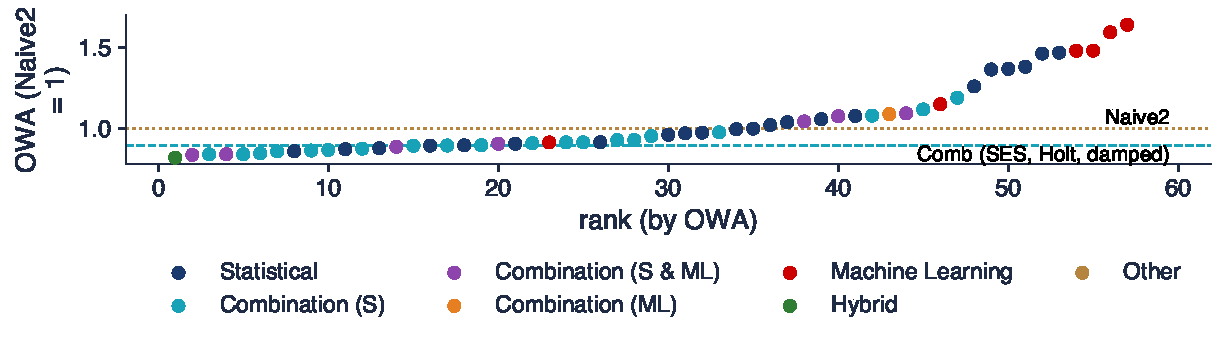
\includegraphics[width=0.97\textwidth,height=0.5\textheight,keepaspectratio]{tsa_ch9_m4.pdf}
\end{center}
\vspace{-0.25cm}
\begin{itemize}
    \item Fișierul oficial de evaluare M4 (github.com/Mcompetitions/M4-methods): OWA pentru cele 59 de metode clasate, propuneri și metode de referință, colorate după tip; 2 metode cu OWA peste 1,7 nu apar pe grafic
\end{itemize}
\quantlet{TSA\_ch9\_case\_studies}{\qlurl{TSA_ch9_case_studies}}
\end{frame}

\begin{frame}{Interpretarea M4}
\itemsize{\small}
\begin{itemize}
    \item Cîștigătorul: modelul hibrid ES-RNN al lui \refSmyl, netezire exponențială în interiorul unui LSTM antrenat pe toate seriile (un model global): OWA 0{,}821, sMAPE 11{,}37\%
    \begin{itemize}
        \item Comb, media metodelor SES, Holt și trend amortizat: OWA 0{,}898, sMAPE 12{,}55\%; Naive2: sMAPE 13{,}56\%
    \end{itemize}
    \item Cele 6 metode ML pure: cea mai bună pe locul 23 (OWA 0{,}915); niciuna nu a depășit Comb, doar una a depășit Naive2 \refMfourA
    \begin{itemize}
        \item 12 dintre cele mai bune 17 metode au fost combinații
    \end{itemize}
    \item Lecția: pe serii scurte și eterogene, combinăm modele statistice sau lăsăm ML să învețe de la toate seriile; ML pur, aplicat local, este mai slab
\end{itemize}
\end{frame}

\begin{frame}{M5: gradient boosting, cel mai precis pe datele din comerț}
\itemsize{\footnotesize}
\begin{columns}[T]
\begin{column}{0.36\textwidth}
\centering

\includegraphics[height=0.42\textheight]{ch9_walmart_store.jpg}\\[1mm]
\imgcap{Un magazin Walmart: datele M5 sînt vînzările zilnice a 3\,049 de produse în 10 magazine}
\imgcredit{https://commons.wikimedia.org/wiki/File:Walmart_store_exterior_5266815680.jpg}{Foto: Walmart Corporate; CC BY 2.0; Wikimedia Commons}
\end{column}
\begin{column}{0.62\textwidth}
\begin{itemize}
    \item 5\,507 echipe din 101 țări; măsura erorii WRMSSE (weighted root mean squared scaled error)
    \begin{itemize}
        \item RMSSE: RMSE a prognozelor raportată la RMSE în eșantion a prognozei naive la un pas
        \item WRMSSE: media RMSSE, ponderată cu valoarea vînzărilor
        \item cîștigătorul (WRMSSE 0,520) a fost cu 22,4\% mai precis decît cea mai bună metodă de referință, netezirea exponențială de jos în sus (0,671)
    \end{itemize}
    \item Cele mai multe metode de top au folosit LightGBM \refLGBM
    \begin{itemize}
        \item cîștigătorul a făcut media unor modele LightGBM combinate pe magazin, categorie și departament, recursive și directe
        \item modele globale, variabile bogate de calendar și preț, multe serii înrudite: condițiile în care ML este superior
    \end{itemize}
\end{itemize}
\end{column}
\end{columns}
\end{frame}

\begin{frame}{Gu, Kelly și Xiu (2020): învățare automată pentru randamentele acțiunilor}
\itemsize{\footnotesize}
\begin{columns}[T]
\begin{column}{0.34\textwidth}
\centering
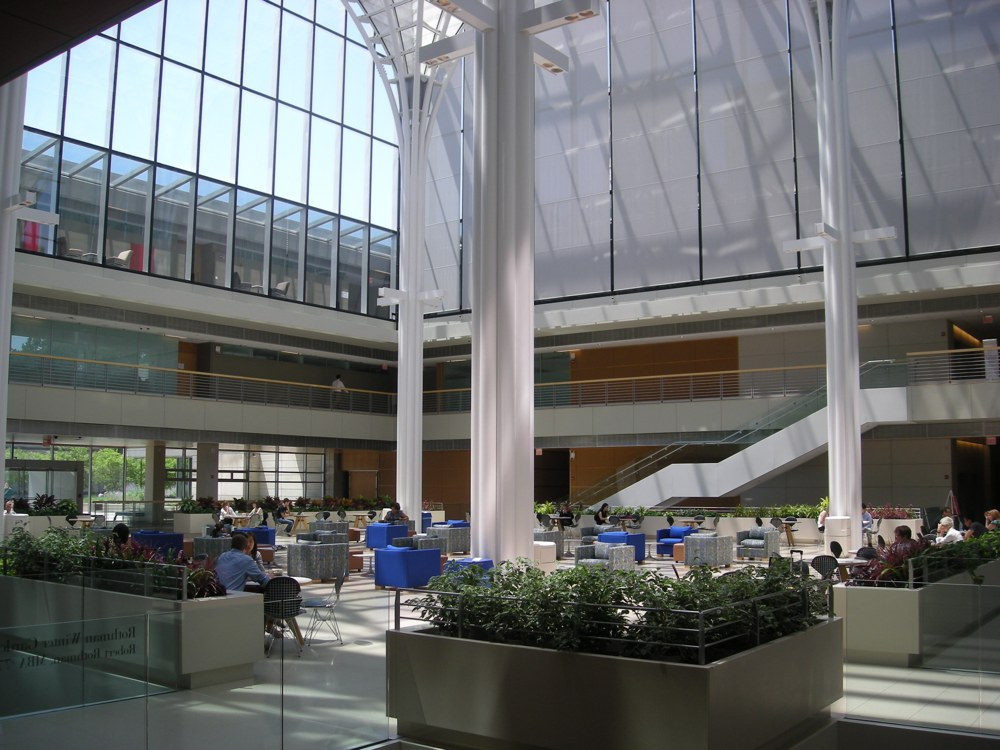
\includegraphics[height=0.36\textheight]{ch9_harper_center_2013.jpg}\\[1mm]
\imgcap{Charles M. Harper Center, University of Chicago Booth School of Business}
\imgcredit{https://commons.wikimedia.org/wiki/File:University_of_Chicago_July_2013_01_(Charles_M._Harper_Center).jpg}{Foto: Michael Barera (2013); CC BY-SA 4.0; Wikimedia Commons}
\end{column}
\begin{column}{0.64\textwidth}
\begin{itemize}
    \item \refGKX: randamentele lunare a circa 30\,000 de acțiuni americane, 1957--2016, 920 de predictori
    \begin{itemize}
        \item 12 metode, de la OLS la rețele neuronale cu cinci straturi
        \item walk-forward: 18 ani de antrenare, 12 de validare, 30 de ani de test, reestimare anuală
    \end{itemize}
    \item $R^2$ lunar în afara eșantionului: cel mult 0,40\% (rețea cu trei straturi); OLS cu toți predictorii: $-3{,}46$\%
    \item $R^2$ mic, valoare mare: un portofoliu long-short ordonat după prognoze atinge un raport Sharpe anual de 1,35 (patru straturi), față de 0,61 pentru OLS-3
    \begin{itemize}
        \item long-short: cumpărăm decila cu cele mai mari prognoze și vindem decila cu cele mai mici
        \item raportul Sharpe: randamentul mediu anual împărțit la abaterea lui standard anuală
    \end{itemize}
\end{itemize}
\end{column}
\end{columns}
\end{frame}

\begin{frame}{Gu, Kelly și Xiu (2020): $R^2$ mic, valoare economică mare}
\itemsize{\footnotesize}
\begin{center}
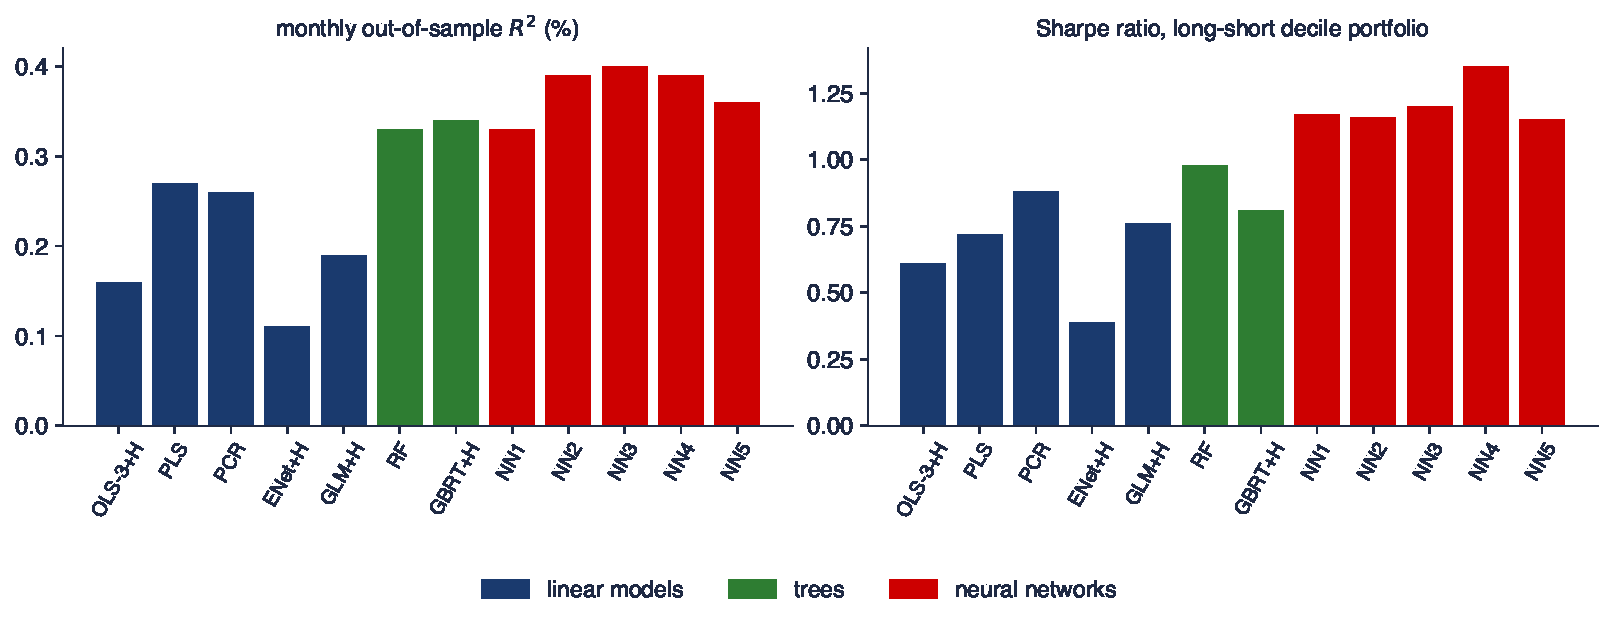
\includegraphics[width=0.97\textwidth,height=0.4\textheight,keepaspectratio]{tsa_ch9_gkx.pdf}
\end{center}
\vspace{-0.25cm}
\begin{itemize}
    \item Cifrele publicate: Tabelul 1 ($R^2$ lunar în afara eșantionului, toate acțiunile) și Tabelul 7 (raportul Sharpe anualizat al portofoliului long-short pe decile, ponderat cu valoarea); +H: funcția de pierdere Huber
    \item OLS-3: OLS pe mărime, raportul valoare contabilă/valoare de piață și momentum; PLS, PCR: partial least squares, regresie pe componente principale; ENet: elastic net
    \item GLM: model liniar generalizat cu spline; RF: random forest; GBRT: arbori de regresie cu gradient boosting; NN1--NN5: rețele cu 1--5 straturi ascunse
\end{itemize}
\quantlet{TSA\_ch9\_case\_studies}{\qlurl{TSA_ch9_case_studies}}
\end{frame}

\begin{frame}{Recapitulare: studii de caz}
\itemsize{\small}
\begin{itemize}
    \item M4: cele mai precise sînt combinațiile și un model hibrid global; ML pur local este mai slab decît metodele simple
    \item M5: modelele globale LightGBM cu variabile de calendar și preț sînt clar cele mai precise
    \item Gu, Kelly și Xiu: predictibilitate mică, dar reală, în secțiunea transversală a acțiunilor; modelele neliniare aduc valoare
\end{itemize}
\end{frame}


%=============================================================================
\section{Contribuția posibilă a AI}
%=============================================================================

\begin{frame}{Foundation models: trimitere la \tsachlinkt{https://danpele.github.io/Time-Series-Analysis/RO/Cursuri/capitol11_foundation_models_serii_timp.pdf}{Capitolul 11}}
\itemsize{\small}
\begin{itemize}
    \item Un \textbf{foundation model} pentru serii de timp este o rețea mare (un transformer) pre-antrenată pe milioane de serii și folosită fără reantrenare (zero-shot)
    \begin{itemize}
        \item modelul global extrem: Chronos, TimesFM, Moirai, Lag-Llama (studiu individual, \tsachlink{https://danpele.github.io/Time-Series-Analysis/RO/Cursuri/capitol11_foundation_models_serii_timp.pdf}{Capitolul 11})
    \end{itemize}
    \item Se aplică aceleași reguli: walk-forward pe date pe care modelul nu le-a văzut la pre-antrenare, aceleași metode de referință, MASE și DM
\end{itemize}
\end{frame}

\begin{frame}{Contribuția posibilă a AI}
\itemsize{\small}
\begin{itemize}
    \item \textbf{Cod}: o primă versiune a tabelului de variabile, a buclei walk-forward și a tabelului de evaluare
    \item \textbf{Explicații}: o a doua explicație a boosting-ului, a porților LSTM sau a predicției conformale
    \item \textbf{Explorare}: multe seturi de variabile și hiperparametri deodată (doar pe datele de validare)
    \item Exemplu de prompt
    \begin{itemize}
        \item \aiprompt{Write Python code that builds lag, rolling-mean and calendar features for daily electricity load, trains HistGradientBoostingRegressor with the direct strategy for horizons 1-14, evaluates it walk-forward against the seasonal naive forecast with MASE and the Diebold-Mariano test, and refits every preprocessing step inside each training window.}
    \end{itemize}
\end{itemize}
\end{frame}

\begin{frame}{Verificări necesare}
\itemsize{\small}
\begin{itemize}
    \item Fiecare variabilă folosește doar date pînă la origine: verificați deplasarea lagurilor și a ferestrelor mobile pe un tabel tipărit
    \item Fără \texttt{KFold(shuffle=True)}, fără scalare sau selecție de variabile estimate pe tot eșantionul
    \item Metodele de referință sînt prezente: naivă sau naivă sezonieră, ETS sau ARIMA, pe aceleași origini
    \item Comparația are un test DM; clasificarea are reperul clasei majoritare
    \item Semințele sînt fixate, iar rezultatul se menține cu o altă sămînță
    \item Fiecare referință citată există: verificați DOI-ul
\end{itemize}
\end{frame}


%=============================================================================
\section{Rezumat}
%=============================================================================

\begin{frame}{Idei de reținut}
\itemsize{\small}
\begin{itemize}
    \item Prognoza ML = învățare supervizată pe un tabel de laguri, statistici pe ferestre mobile și variabile de calendar cunoscute la origine
    \item Doar validare walk-forward; leakage-ul produce scoruri spectaculoase și false
    \item Ridge și lasso, random forest, GB, MLP, LSTM: fiecare are un parametru de complexitate fixat prin validare
    \item Arborii nu pot extrapola: modelăm variații, nu niveluri
    \item Datele noastre: modelele liniare cu variabile bune au cel puțin aceeași precizie ca ML pentru consum și inflație; ML ajută pentru volatilitate; niciun model nu prognozează semnul randamentelor
    \item ML este superior cînd există multe serii înrudite (modele globale, hibridul din M4, LightGBM în M5); comparăm întotdeauna cu metode de referință, MASE și DM
\end{itemize}
\end{frame}

\begin{frame}{Formule de reținut}
\itemsize{\small}
{\renewcommand{\arraystretch}{1.35}\begin{center}
\footnotesize
\begin{tabular}{ll}
\toprule
\textbf{Mărimea} & \textbf{Formula} \\
\midrule
Prognoza directă & $\hat y_{T+h} = \hat f_h(y_T, \dots, y_{T-p+1}, \mathbf{z}_{T+h})$, $\mathbf{z}_{T+h}$: variabilele de calendar \\
Ridge, lasso & $\min \sum_t (y_t - \mathbf{x}_t'\beta)^2 + \lambda\sum_j\beta_j^2$; \quad $+ \lambda\sum_j|\beta_j|$ \\
Deplasare--varianță & $E[(y_0 - \hat f(x_0))^2] = \text{deplasare}^2 + \Var(\hat f(x_0)) + \sigma^2$ \\
Boosting & $F_m(\mathbf{x}) = F_{m-1}(\mathbf{x}) + \nu\,g_m(\mathbf{x})$ \\
MLP & $\hat y = c + \sum_j v_j\,g(b_j + \mathbf{w}_j'\mathbf{x})$ \\
LSTM & $c_t = f_t \odot c_{t-1} + i_t \odot \tilde c_t$, \quad $h_t = o_t \odot \tanh(c_t)$ \\
Funcția pinball & $L_\tau(y, q) = \max(\tau(y - q), (\tau - 1)(y - q))$ \\
Predicția conformală & $\hat y \pm \hat q$, \quad $\hat q = |e|_{(\lceil (n+1)(1-\alpha) \rceil)}$ \\
MASE & $\text{MAE} / \frac{1}{n-m}\sum_{t>m}|y_t - y_{t-m}|$ \\
\bottomrule
\end{tabular}
\end{center}
}
\end{frame}

\begin{frame}{Autoevaluare}
\itemsize{\small}
\begin{itemize}
    \item \textbf{Întrebare}: o medie mobilă pe 7 zile centrată în $t$ este folosită ca variabilă pentru $y_{t+1}$. Este permis?
    \begin{itemize}
        \item \textbf{Răspuns}: nu: conține $y_{t+1}, y_{t+2}, y_{t+3}$; folosiți media $y_{t-6}, \dots, y_t$
    \end{itemize}
    \item \textbf{Întrebare}: un random forest antrenat pe nivelurile PIB-ului pînă în 2019 prognozează anul 2024. Ce nu funcționează?
    \begin{itemize}
        \item \textbf{Răspuns}: prognoza lui nu poate depăși cel mai mare nivel văzut la antrenare; modelați ratele de creștere
    \end{itemize}
    \item \textbf{Întrebare}: un clasificator prognozează semnul randamentelor zilnice cu acuratețea de 53\%. Este util?
    \begin{itemize}
        \item \textbf{Răspuns}: doar dacă depășește semnificativ ponderea zilelor de creștere în perioada de test (circa 54\% pentru S\&P 500)
    \end{itemize}
    \item Urmează: \tsachlink{https://danpele.github.io/Time-Series-Analysis/RO/Cursuri/capitol10_spatiul_starilor_kalman_markov_switching.pdf}{Capitolul 10}, modele în spațiul stărilor, filtrul Kalman și modele Markov switching
\end{itemize}
\end{frame}


%=============================================================================
\section{Bibliografie}
%=============================================================================

\begin{frame}{Bibliografie (1/3)}
\itemsize{\tiny}
\begin{itemize}
    \item Ben Taieb, S., Bontempi, G., Atiya, A. F., \& Sorjamaa, A. (2012). A review and comparison of strategies for multi-step ahead time series forecasting based on the NN5 forecasting competition. \textit{Expert Systems with Applications}, 39(8), 7067--7083. \href{https://doi.org/10.1016/j.eswa.2012.01.039}{doi:10.1016/j.eswa.2012.01.039}
    \item Bergmeir, C., Hyndman, R. J., \& Koo, B. (2018). A note on the validity of cross-validation for evaluating autoregressive time series prediction. \textit{Computational Statistics \& Data Analysis}, 120, 70--83. \href{https://doi.org/10.1016/j.csda.2017.11.003}{doi:10.1016/j.csda.2017.11.003}
    \item Breiman, L. (2001). Random forests. \textit{Machine Learning}, 45(1), 5--32. \href{https://doi.org/10.1023/A:1010933404324}{doi:10.1023/A:1010933404324}
    \item Chen, T., \& Guestrin, C. (2016). XGBoost: A scalable tree boosting system. \textit{Proceedings of the 22nd ACM SIGKDD International Conference on Knowledge Discovery and Data Mining}, 785--794. \href{https://doi.org/10.1145/2939672.2939785}{doi:10.1145/2939672.2939785}
    \item Corsi, F. (2009). A simple approximate long-memory model of realized volatility. \textit{Journal of Financial Econometrics}, 7(2), 174--196. \href{https://doi.org/10.1093/jjfinec/nbp001}{doi:10.1093/jjfinec/nbp001}
    \item Diebold, F. X., \& Mariano, R. S. (1995). Comparing predictive accuracy. \textit{Journal of Business \& Economic Statistics}, 13(3), 253--263. \href{https://doi.org/10.1080/07350015.1995.10524599}{doi:10.1080/07350015.1995.10524599}
    \item Friedman, J. H. (2001). Greedy function approximation: A gradient boosting machine. \textit{The Annals of Statistics}, 29(5), 1189--1232. \href{https://doi.org/10.1214/aos/1013203451}{doi:10.1214/aos/1013203451}
    \item Garman, M. B., \& Klass, M. J. (1980). On the estimation of security price volatilities from historical data. \textit{The Journal of Business}, 53(1), 67--78. \href{https://doi.org/10.1086/296072}{doi:10.1086/296072}
    \item Gu, S., Kelly, B., \& Xiu, D. (2020). Empirical asset pricing via machine learning. \textit{The Review of Financial Studies}, 33(5), 2223--2273. \href{https://doi.org/10.1093/rfs/hhaa009}{doi:10.1093/rfs/hhaa009}
    \item Harvey, D., Leybourne, S., \& Newbold, P. (1997). Testing the equality of prediction mean squared errors. \textit{International Journal of Forecasting}, 13(2), 281--291. \href{https://doi.org/10.1016/S0169-2070(96)00719-4}{doi:10.1016/S0169-2070(96)00719-4}
    \item Hastie, T., Tibshirani, R., \& Friedman, J. (2009). \textit{The Elements of Statistical Learning} (2nd ed.). Springer. \href{https://doi.org/10.1007/978-0-387-84858-7}{doi:10.1007/978-0-387-84858-7}
    \item Hewamalage, H., Bergmeir, C., \& Bandara, K. (2021). Recurrent neural networks for time series forecasting: Current status and future directions. \textit{International Journal of Forecasting}, 37(1), 388--427. \href{https://doi.org/10.1016/j.ijforecast.2020.06.008}{doi:10.1016/j.ijforecast.2020.06.008}
\end{itemize}
\end{frame}

\begin{frame}{Bibliografie (2/3)}
\itemsize{\tiny}
\begin{itemize}
    \item Hochreiter, S., \& Schmidhuber, J. (1997). Long short-term memory. \textit{Neural Computation}, 9(8), 1735--1780. \href{https://doi.org/10.1162/neco.1997.9.8.1735}{doi:10.1162/neco.1997.9.8.1735}
    \item Hoerl, A. E., \& Kennard, R. W. (1970). Ridge regression: Biased estimation for nonorthogonal problems. \textit{Technometrics}, 12(1), 55--67. \href{https://doi.org/10.1080/00401706.1970.10488634}{doi:10.1080/00401706.1970.10488634}
    \item Hornik, K., Stinchcombe, M., \& White, H. (1989). Multilayer feedforward networks are universal approximators. \textit{Neural Networks}, 2(5), 359--366. \href{https://doi.org/10.1016/0893-6080(89)90020-8}{doi:10.1016/0893-6080(89)90020-8}
    \item Huang, C., \& Petukhina, A. (2022). \textit{Applied Time Series Analysis and Forecasting with Python}. Springer. \href{https://doi.org/10.1007/978-3-031-13584-2}{doi:10.1007/978-3-031-13584-2}
    \item Hyndman, R. J., \& Athanasopoulos, G. (2021). \textit{Forecasting: Principles and Practice} (3rd ed.), Section 12.4, Neural network models. OTexts. \href{https://otexts.com/fpp3/nnetar.html}{otexts.com/fpp3/nnetar.html}
    \item Hyndman, R. J., \& Koehler, A. B. (2006). Another look at measures of forecast accuracy. \textit{International Journal of Forecasting}, 22(4), 679--688. \href{https://doi.org/10.1016/j.ijforecast.2006.03.001}{doi:10.1016/j.ijforecast.2006.03.001}
    \item Januschowski, T., Gasthaus, J., Wang, Y., Salinas, D., Flunkert, V., Bohlke-Schneider, M., \& Callot, L. (2020). Criteria for classifying forecasting methods. \textit{International Journal of Forecasting}, 36(1), 167--177. \href{https://doi.org/10.1016/j.ijforecast.2019.05.008}{doi:10.1016/j.ijforecast.2019.05.008}
    \item Kaufman, S., Rosset, S., Perlich, C., \& Stitelman, O. (2012). Leakage in data mining: Formulation, detection, and avoidance. \textit{ACM Transactions on Knowledge Discovery from Data}, 6(4), 1--21. \href{https://doi.org/10.1145/2382577.2382579}{doi:10.1145/2382577.2382579}
    \item Ke, G., Meng, Q., Finley, T., Wang, T., Chen, W., Ma, W., Ye, Q., \& Liu, T.-Y. (2017). LightGBM: A highly efficient gradient boosting decision tree. \textit{Advances in Neural Information Processing Systems}, 30. \href{https://proceedings.neurips.cc/paper/2017/hash/6449f44a102fde848669bdd9eb6b76fa-Abstract.html}{proceedings.neurips.cc}
    \item Koenker, R., \& Bassett, G. (1978). Regression quantiles. \textit{Econometrica}, 46(1), 33--50. \href{https://doi.org/10.2307/1913643}{doi:10.2307/1913643}
    \item Lei, J., G'Sell, M., Rinaldo, A., Tibshirani, R. J., \& Wasserman, L. (2018). Distribution-free predictive inference for regression. \textit{Journal of the American Statistical Association}, 113(523), 1094--1111. \href{https://doi.org/10.1080/01621459.2017.1307116}{doi:10.1080/01621459.2017.1307116}
    \item Lim, B., \& Zohren, S. (2021). Time-series forecasting with deep learning: A survey. \textit{Philosophical Transactions of the Royal Society A}, 379(2194), 20200209. \href{https://doi.org/10.1098/rsta.2020.0209}{doi:10.1098/rsta.2020.0209}
\end{itemize}
\end{frame}

\begin{frame}{Bibliografie (3/3)}
\itemsize{\tiny}
\begin{itemize}
    \item Makridakis, S., Spiliotis, E., \& Assimakopoulos, V. (2018a). Statistical and machine learning forecasting methods: Concerns and ways forward. \textit{PLOS ONE}, 13(3), e0194889. \href{https://doi.org/10.1371/journal.pone.0194889}{doi:10.1371/journal.pone.0194889}
    \item Makridakis, S., Spiliotis, E., \& Assimakopoulos, V. (2018b). The M4 Competition: Results, findings, conclusion and way forward. \textit{International Journal of Forecasting}, 34(4), 802--808. \href{https://doi.org/10.1016/j.ijforecast.2018.06.001}{doi:10.1016/j.ijforecast.2018.06.001}
    \item Makridakis, S., Spiliotis, E., \& Assimakopoulos, V. (2020). The M4 Competition: 100,000 time series and 61 forecasting methods. \textit{International Journal of Forecasting}, 36(1), 54--74. \href{https://doi.org/10.1016/j.ijforecast.2019.04.014}{doi:10.1016/j.ijforecast.2019.04.014}
    \item Makridakis, S., Spiliotis, E., \& Assimakopoulos, V. (2022). M5 accuracy competition: Results, findings, and conclusions. \textit{International Journal of Forecasting}, 38(4), 1346--1364. \href{https://doi.org/10.1016/j.ijforecast.2021.11.013}{doi:10.1016/j.ijforecast.2021.11.013}
    \item Medeiros, M. C., Vasconcelos, G. F. R., Veiga, \'A., \& Zilberman, E. (2021). Forecasting inflation in a data-rich environment: The benefits of machine learning methods. \textit{Journal of Business \& Economic Statistics}, 39(1), 98--119. \href{https://doi.org/10.1080/07350015.2019.1637745}{doi:10.1080/07350015.2019.1637745}
    \item Montero-Manso, P., \& Hyndman, R. J. (2021). Principles and algorithms for forecasting groups of time series: Locality and globality. \textit{International Journal of Forecasting}, 37(4), 1632--1653. \href{https://doi.org/10.1016/j.ijforecast.2021.03.004}{doi:10.1016/j.ijforecast.2021.03.004}
    \item Patton, A. J. (2011). Volatility forecast comparison using imperfect volatility proxies. \textit{Journal of Econometrics}, 160(1), 246--256. \href{https://doi.org/10.1016/j.jeconom.2010.03.034}{doi:10.1016/j.jeconom.2010.03.034}
    \item Rumelhart, D. E., Hinton, G. E., \& Williams, R. J. (1986). Learning representations by back-propagating errors. \textit{Nature}, 323(6088), 533--536. \href{https://doi.org/10.1038/323533a0}{doi:10.1038/323533a0}
    \item Salinas, D., Flunkert, V., Gasthaus, J., \& Januschowski, T. (2020). DeepAR: Probabilistic forecasting with autoregressive recurrent networks. \textit{International Journal of Forecasting}, 36(3), 1181--1191. \href{https://doi.org/10.1016/j.ijforecast.2019.07.001}{doi:10.1016/j.ijforecast.2019.07.001}
    \item Smyl, S. (2020). A hybrid method of exponential smoothing and recurrent neural networks for time series forecasting. \textit{International Journal of Forecasting}, 36(1), 75--85. \href{https://doi.org/10.1016/j.ijforecast.2019.03.017}{doi:10.1016/j.ijforecast.2019.03.017}
    \item Tibshirani, R. (1996). Regression shrinkage and selection via the lasso. \textit{Journal of the Royal Statistical Society: Series B}, 58(1), 267--288. \href{https://doi.org/10.1111/j.2517-6161.1996.tb02080.x}{doi:10.1111/j.2517-6161.1996.tb02080.x}
\end{itemize}
\end{frame}

\end{document}
